%Compile with XeLatex
\documentclass[11pt]{scrartcl} % Font size


%----------------------------------------------------------------------------------------
%	PACKAGES AND OTHER DOCUMENT CONFIGURATIONS
%----------------------------------------------------------------------------------------

\usepackage{amsmath, amsfonts, amsthm} % Math packages

\usepackage{listings} % Code listings, with syntax highlighting
\lstset{ 
	language=Matlab, % choose the language of the code
%	basicstyle=10pt, % the size of the fonts that are used for the code
	numbers=left,    % where to put the line-numbers
	numberstyle=\footnotesize,% the size of the fonts that are used for the line-numbers
	stepnumber=1,% the step between two line-numbers. If it's 1 each line will be numbered
	numbersep=5pt,% how far the line-numbers are from the code
%	backgroundcolor=\color{white},  	% choose the background color. You must add \usepackage{color}
	showspaces=false, % show spaces adding particular underscores
	showstringspaces=false,% underline spaces within strings
	showtabs=false,% show tabs within strings adding particular underscores
%	frame=single,	% adds a frame around the code
%	tabsize=2, 		% sets default tabsize to 2 spaces
%	captionpos=b, 			% sets the caption-position to bottom
	breaklines=true,   			% sets automatic line breaking
	breakatwhitespace=false, % sets if automatic breaks should only happen at whitespace
	escapeinside={\%*}{*)} % if you want to add a comment within your code
}
\usepackage{fontspec,xgreek,polyglossia}
\usepackage{fancyvrb}
\usepackage{hyperref}
\setdefaultlanguage{greek}
\setotherlanguage[]{english} % Greek (main) and English language hyphenation
\setmainfont{Times New Roman}
\setsansfont{Arial}
\setmonofont{DejaVu Sans Mono}
\newfontfamily\greekfont[Script=Greek]{Linux Libertine O}
\newfontfamily\greekfontsf[Script=Greek]{Linux Libertine O}
\usepackage{graphicx} % Required for inserting images
\usepackage{float}
\graphicspath{{Figures/}{./}} % Specifies where to look for included images (trailing slash required)

\usepackage{booktabs} % Required for better horizontal rules in tables

\numberwithin{equation}{section} % Number equations within sections (i.e. 1.1, 1.2, 2.1, 2.2 instead of 1, 2, 3, 4)
\numberwithin{figure}{section} % Number figures within sections (i.e. 1.1, 1.2, 2.1, 2.2 instead of 1, 2, 3, 4)
\numberwithin{table}{section} % Number tables within sections (i.e. 1.1, 1.2, 2.1, 2.2 instead of 1, 2, 3, 4)

\setlength\parindent{0pt} % Removes all indentation from paragraphs

\usepackage{enumitem} % Required for list customisation
\setlist{noitemsep} % No spacing between list items

%----------------------------------------------------------------------------------------
%	DOCUMENT MARGINS
%----------------------------------------------------------------------------------------

\usepackage{geometry} % Required for adjusting page dimensions and margins

\geometry{
	paper=a4paper, % Paper size, change to letterpaper for US letter size
	top=2.5cm, % Top margin
	bottom=3cm, % Bottom margin
	left=3cm, % Left margin
	right=3cm, % Right margin
	headheight=0.75cm, % Header height
	footskip=1.5cm, % Space from the bottom margin to the baseline of the footer
	headsep=0.75cm, % Space from the top margin to the baseline of the header
	%showframe, % Uncomment to show how the type block is set on the page
}

%----------------------------------------------------------------------------------------
%	FONTS
%----------------------------------------------------------------------------------------

\usepackage[utf8]{inputenc} % Required for inputting international characters
%\usepackage[T1]{fontenc} % Use 8-bit encoding

\usepackage{fourier} % Use the Adobe Utopia font for the document

%----------------------------------------------------------------------------------------
%	SECTION TITLES
%----------------------------------------------------------------------------------------

\usepackage{sectsty} % Allows customising section commands

\sectionfont{\vspace{6pt}\centering\normalfont\scshape} % \section{} styling
\subsectionfont{\normalfont\bfseries} % \subsection{} styling
\subsubsectionfont{\normalfont\itshape} % \subsubsection{} styling
\paragraphfont{\normalfont\scshape} % \paragraph{} styling

%----------------------------------------------------------------------------------------
%	HEADERS AND FOOTERS
%----------------------------------------------------------------------------------------

\usepackage{scrlayer-scrpage} % Required for customising headers and footers

\ohead*{} % Right header
\ihead*{} % Left header
\chead*{} % Centre header

\ofoot*{} % Right footer
\ifoot*{} % Left footer
\cfoot*{\pagemark} % Centre footer
 % Include the file specifying the document structure and custom commands

\title{	
	\normalfont\normalsize
	\textsc{ Αριστοτέλειο Πανεπιστήμιο Θεσσαλονίκης, Σχολή Θετικών Επιστημών, Τμήμα Φυσικής}\\ % Your university, school and/or department name(s)
	\vspace{25pt} % Whitespace
	\rule{\linewidth}{0.5pt}\\ % Thin top horizontal rule
	\vspace{20pt} % Whitespace
	{\huge Εργασία στο Μάθημα Ανάλυση Δεδομένων }\\ % The assignment title
	\vspace{12pt} % Whitespace
	\rule{\linewidth}{2pt}\\ % Thick bottom horizontal rule
	\vspace{12pt} % Whitespace
}

\author{\LARGE Κίμων Ζαγκούρης \\ A.E.M. 4353 \\ Email: kzagko@gmail.com} % Your name

\date{\normalsize\today} % Today's date (\today) or a custom date

\begin{document}

\maketitle


\begin{figure}[H]
	\centering
	\includegraphics[width=0.7\columnwidth]{Main.jpg}
\end{figure}
\footnote{Image created by Timashov Sergiy.}
\pagenumbering{gobble}
\newpage


\tableofcontents
\newpage
\pagenumbering{arabic}


\section{Ζητήματα}
\label{sec:z}
Παρακάτω είναι τα 10 ζητήματα της εργασίας αυτής ανά κεφάλαιο. Στο \hyperref[sec:Prog]{Κεφάλαιο \ref*{sec:Prog}} υπάρχουν τα αντίστοιχα προγράμματα Matlab που χρησιμοποιήθηκαν για την επίλυση των ζητημάτων. Στα προγράμματα υπάρχουν σχόλια  για την καλύτερη παρακολούθηση του κώδικα σε κάποια σημεία.


\subsection{Ζήτημα 1}
\label{subsec:z1}
Στο ζήτημα αυτό τρέχουμε τον παρακάτω \hyperref[mat:1]{Κώδικα} για 6 περιπτώσεις και παραθέτουμε τα γραφήματα.

\begin{figure}[H] 

	\centering
	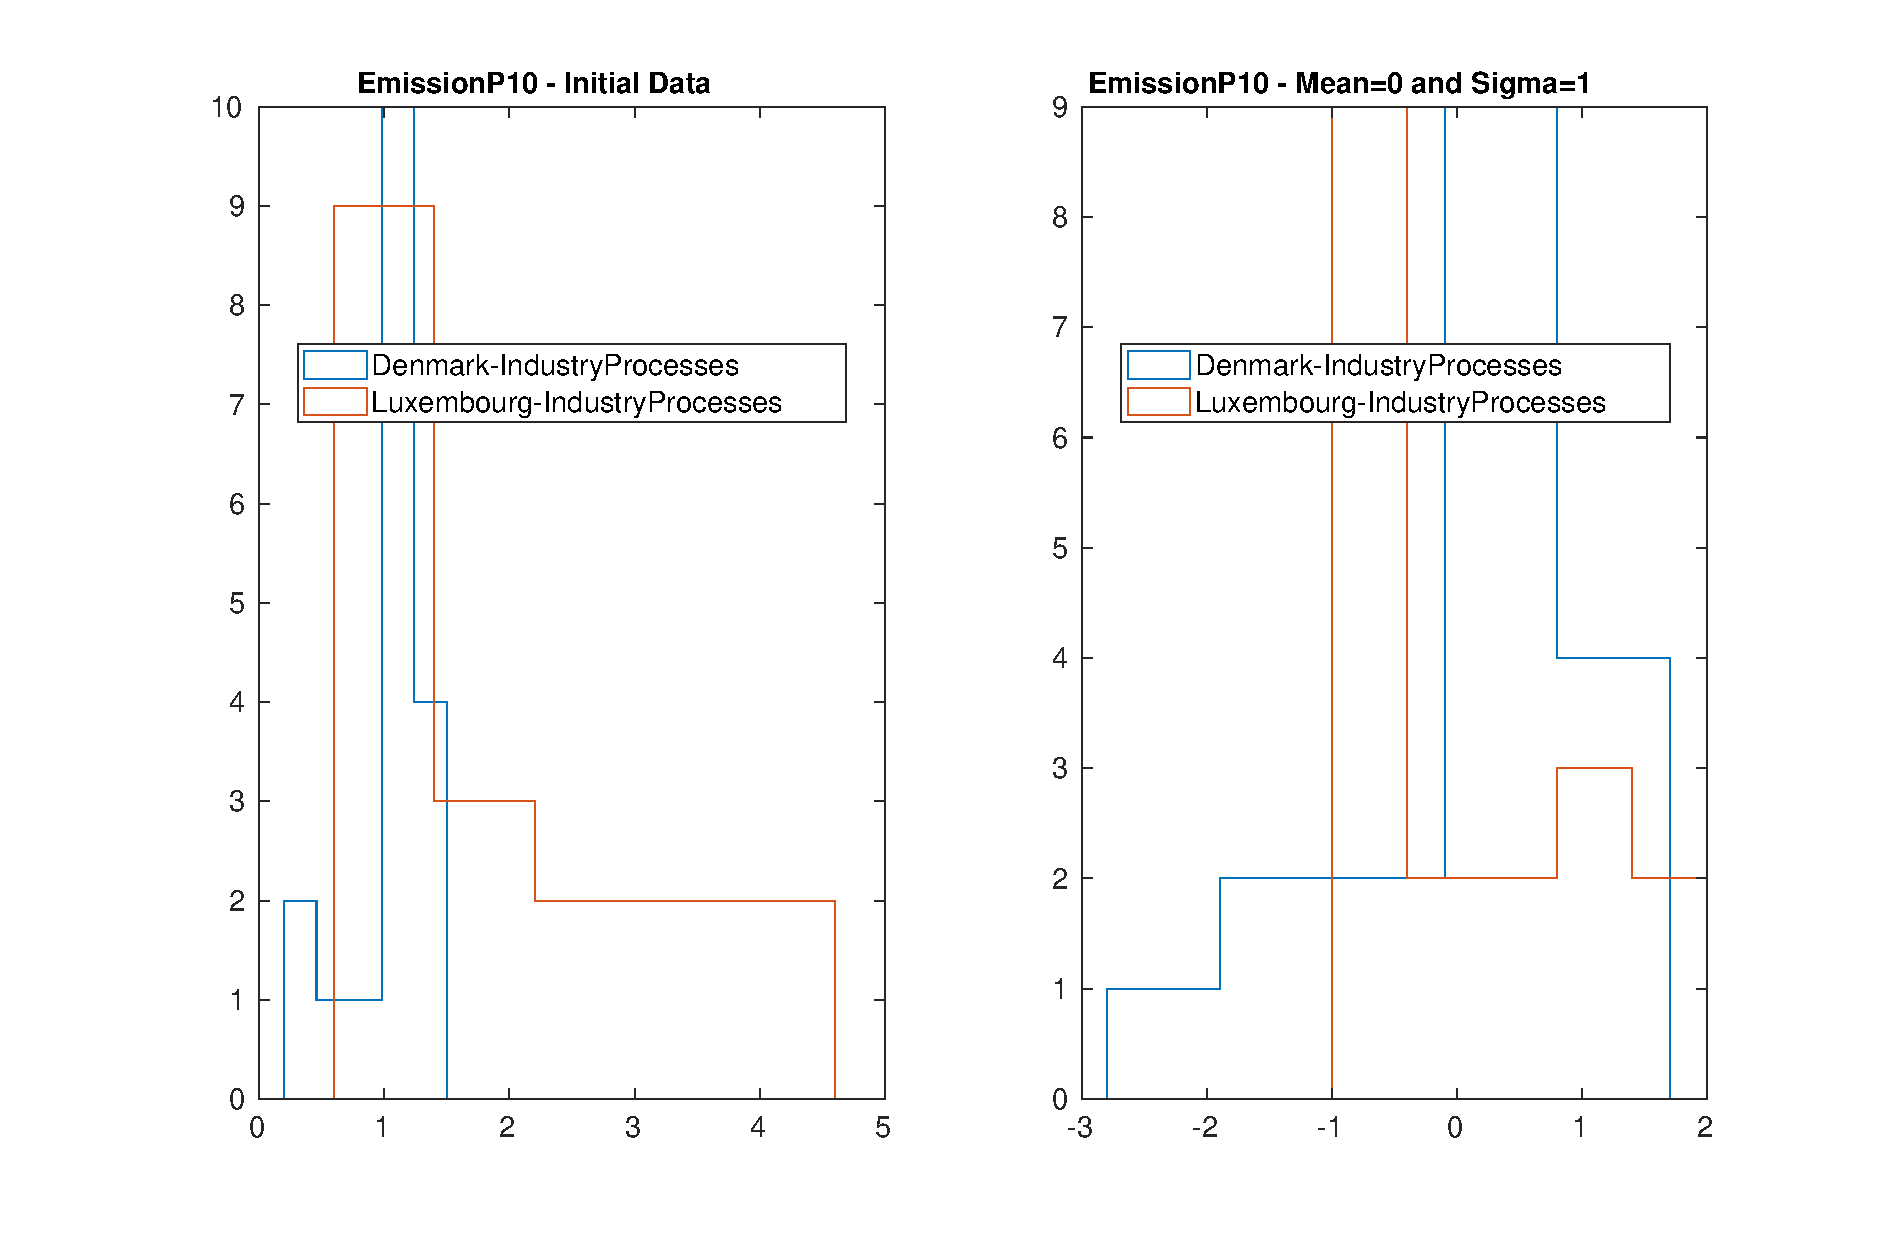
\includegraphics[width=1\columnwidth]{Ex1/Denmark_Luxembourg_IndustryProcesses_hist.eps}	
	\caption{PM10 Emissions for Denmark Luxembourg IndustryProcesses. }
	\label{fig:z1}
\end{figure}

\begin{figure}[H] 

	\centering
	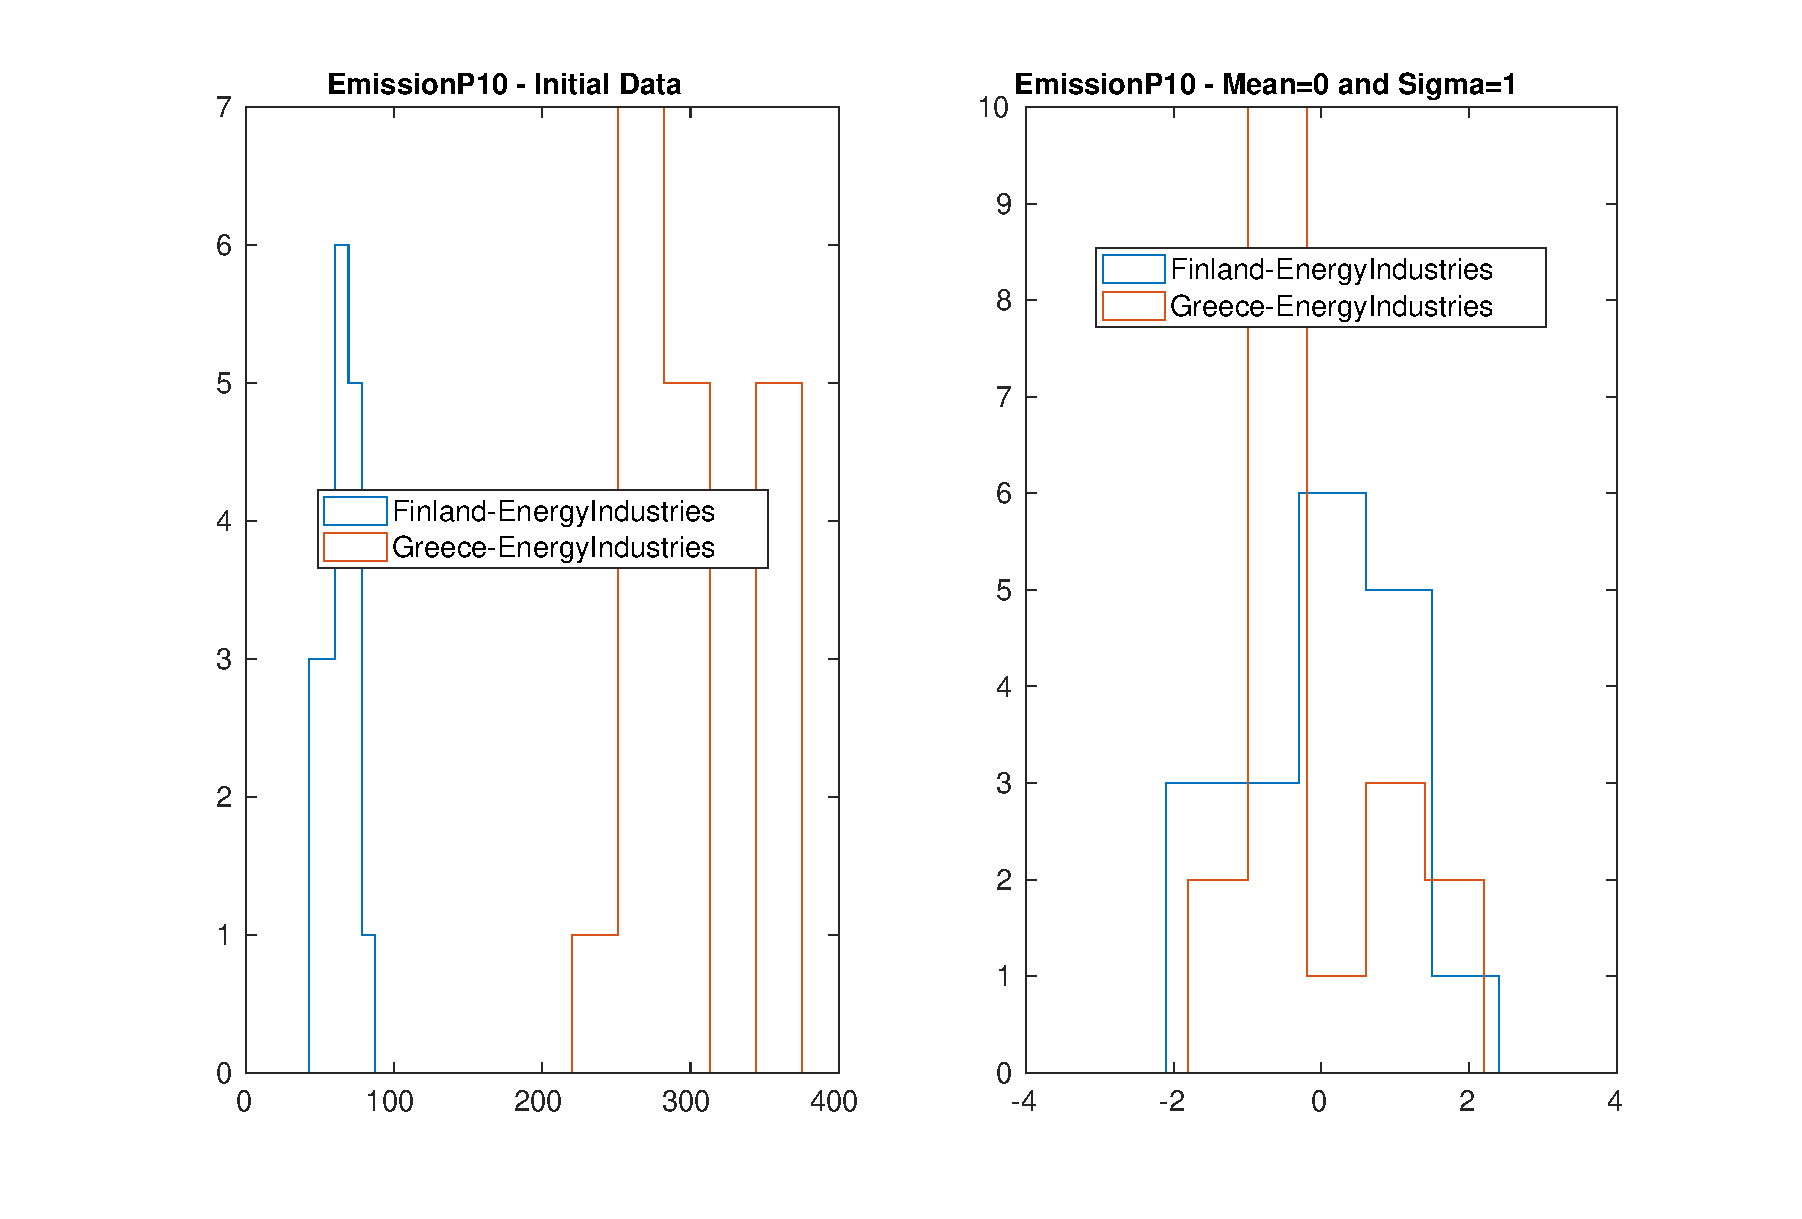
\includegraphics[width=1\columnwidth]{Ex1/Finland_Greece_EnergyIndustries_hist.eps}	
	\caption{PM10 Emissions for Finland Greece EnergyIndustries.}
	\label{fig:z2}
\end{figure}

\begin{figure}[H] 

	\centering
	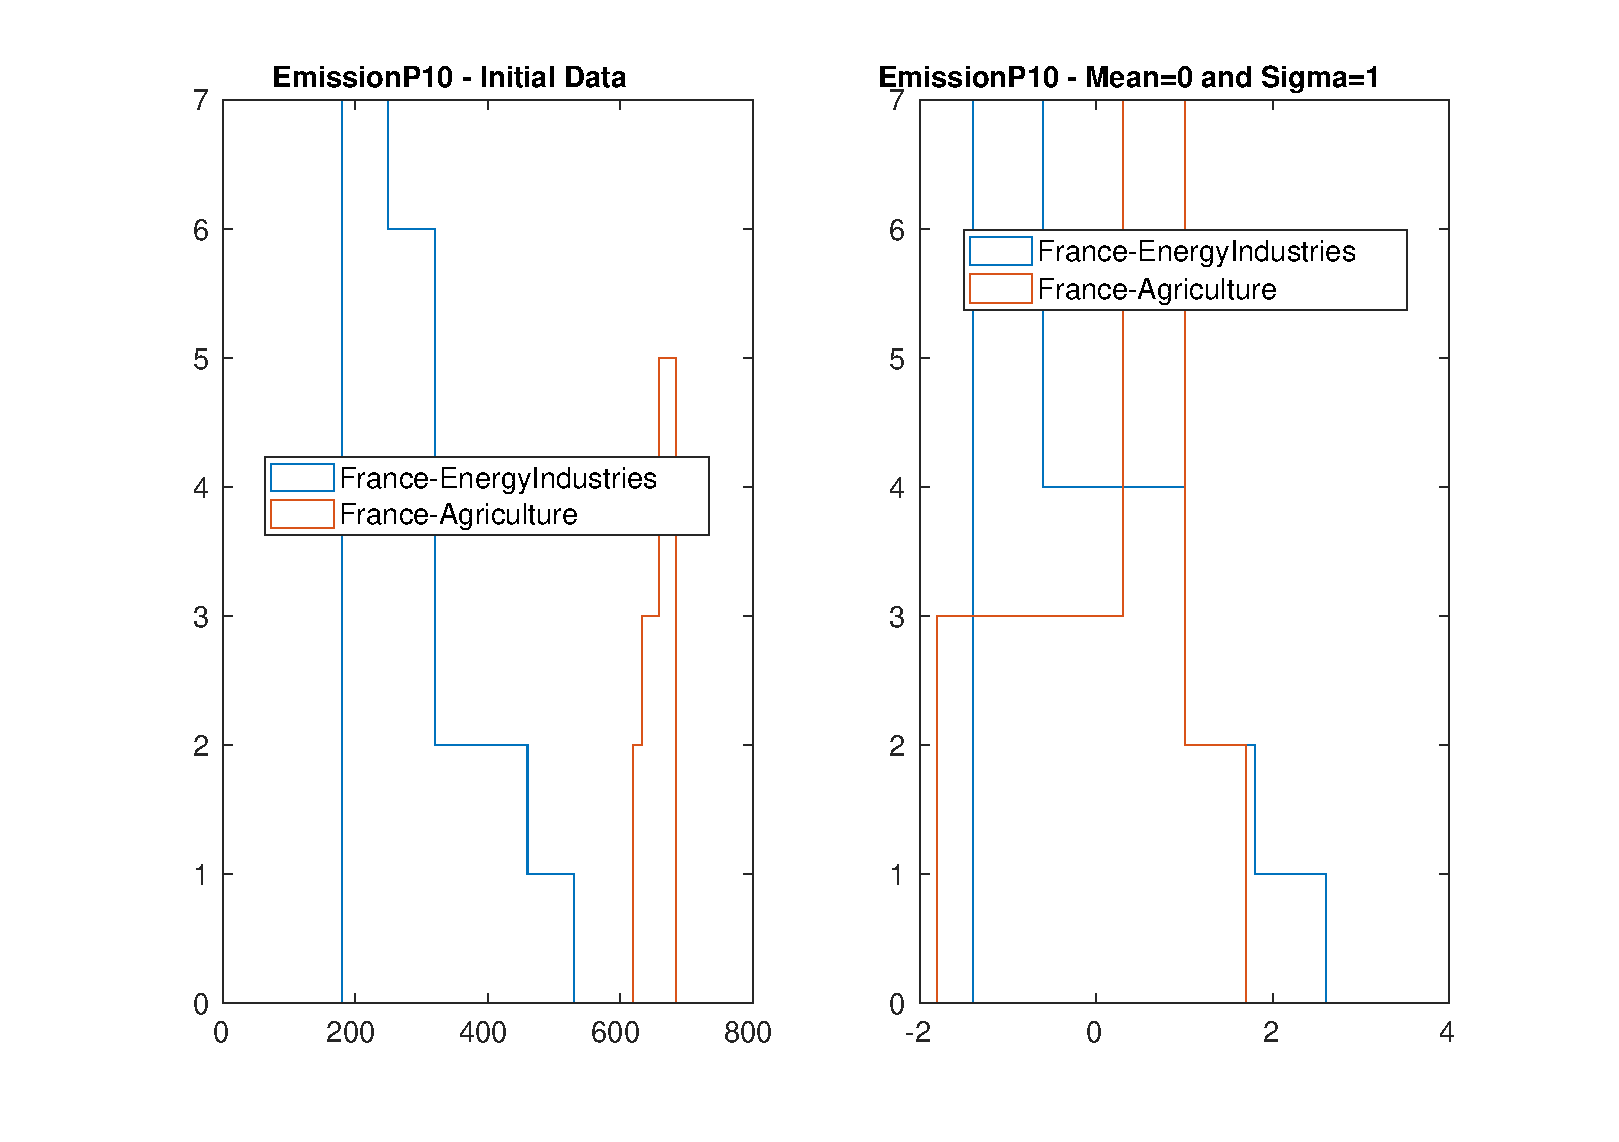
\includegraphics[width=1\columnwidth]{Ex1/France_EnergyIndustries_Agriculture_hist.eps}	
\caption{PM10 Emissions for France EnergyIndustries Agriculture.}
	\label{fig:z3}
\end{figure}


\begin{figure}[H]

	\centering
	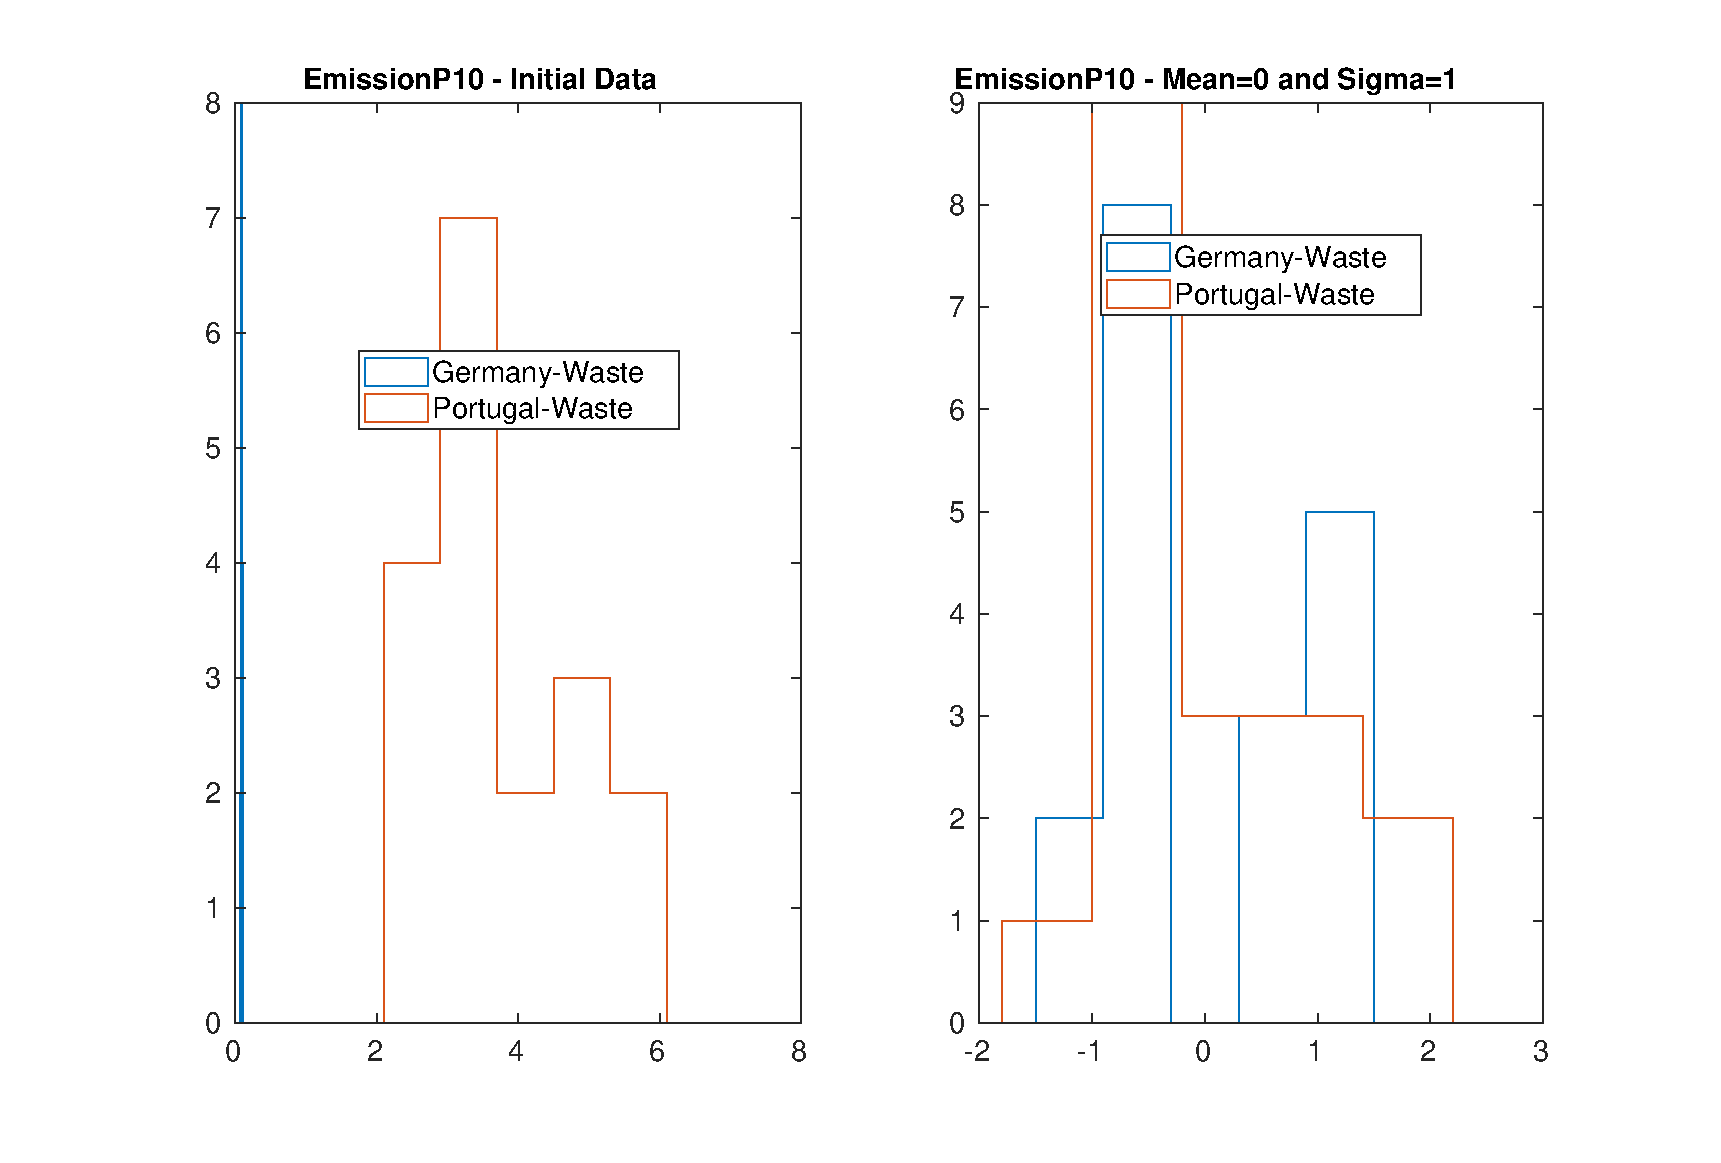
\includegraphics[width=1\columnwidth]{Ex1/Germany_Portugal_Waste_hist.eps}	
\caption{PM10 Emissions for Germany Portugal Waste.}
\label{fig:z4} 
\end{figure}


\begin{figure}[H] 

	\centering
	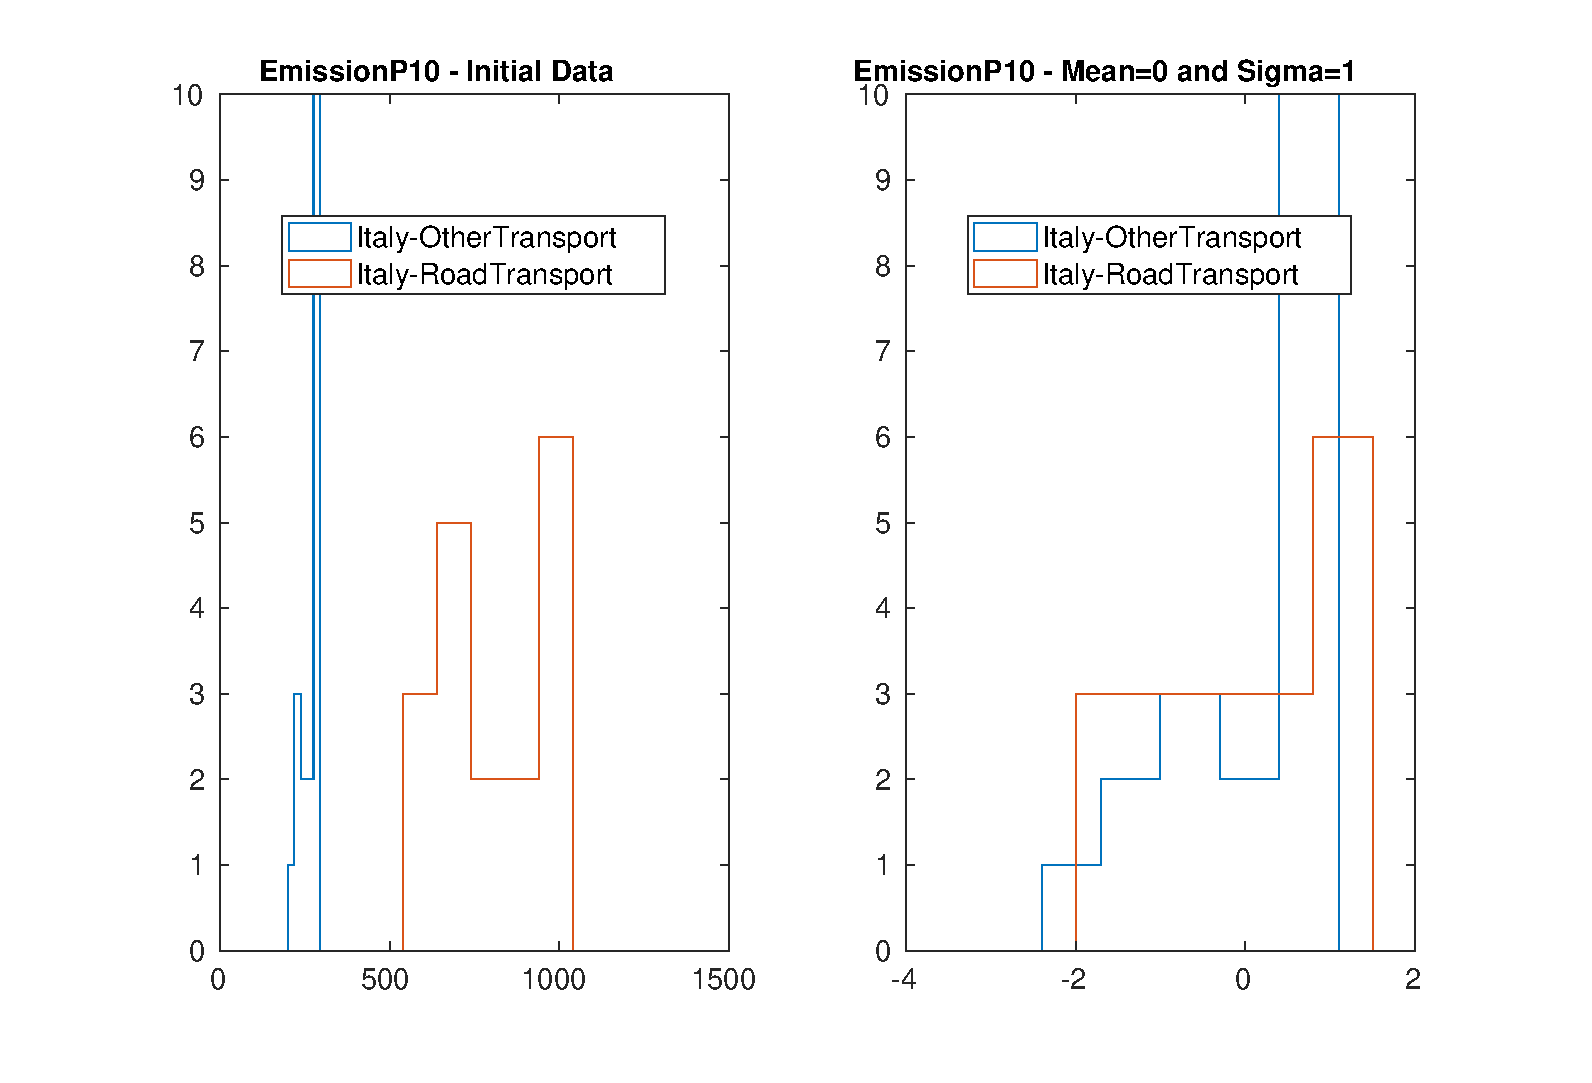
\includegraphics[width=1\columnwidth]{Ex1/Italy_OtherTransport_RoadTransport_hist.eps}	
	\caption{PM10 Emissions for Italy OtherTransport RoadTransport.}
		\label{fig:z5}
\end{figure}

\begin{figure}[H]

	\centering
	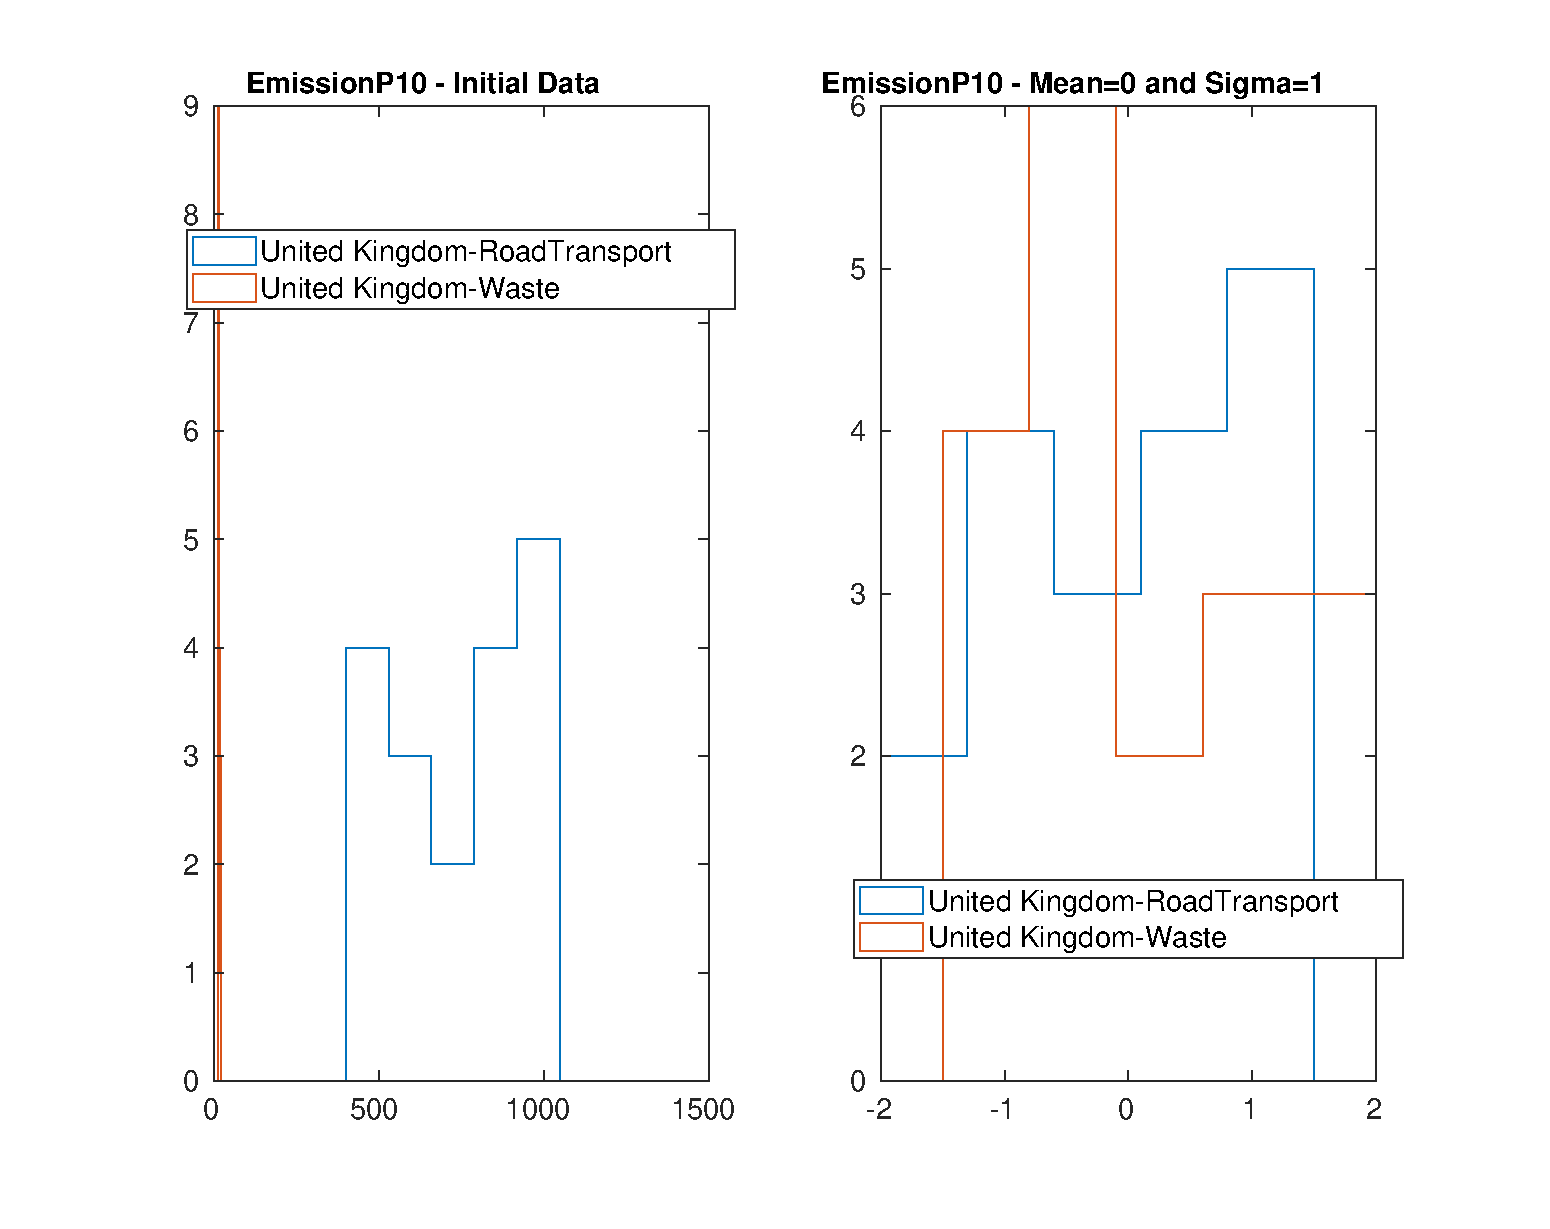
\includegraphics[width=1\columnwidth]{Ex1/United-Kingdom_RoadTransport_Waste_hist.eps}	
\caption{PM10 Emissions for United Kingdom RoadTransport Waste.}
\label{fig:z6} 
\end{figure}


Τα παραπάνω αποτελούν ένα τυχαίο δείγμα από όλα τα δυνατά αποτελέσματα και συνδυασμούς των χωρών και των δραστηριοτήτων αλλά μπορούμε να σχολιάσουμε μερικά από αυτά. Στο \hyperref[fig:z3]{σχήμα \ref*{fig:z3}} βλέπουμε ότι οι κατανομές των PM10 πριν την κανονικοποίηση δεν είναι εύκολο να συγκριθούν και να ελεγχθούν αλλά μετά την κανονικοποίηση μπορούμε να πούμε ότι φαίνεται να μην έχουν κοινή κατανομή λόγω του σχήματός τους. Ενώ αντίθετα στο \hyperref[fig:z5]{σχήμα \ref*{fig:z5}} Για την κατανομή των PM10 στην Ιταλία βλέπουμε ότι όταν κανονικοποιούμε τις κατανομές φαίνεται αυτές να μοιάζουν. Γενικά όμως τα δεδομένα είναι λίγα, στην καλύτερη περίπτωση 18 σημεία, τα οποία όταν κατανέμονται σε ιστόγραμμα δίνουν πολύ μικρό αριθμό στοιχείων, περίπου 4, ανά περιοχή κατανομής (bin). Με αποτέλεσμα να είναι δύσκολο να έχουμε καλή περιγραφή της κάθε κατανομής. 

\subsection{Ζήτημα 2}
\label{subsec:z2}
Για την επίλυση αυτού του ζητήματος κάνουμε χρήση του \hyperref[mat:2]{κώδικα \ref*{mat:2}}. Λόγου του μικρού αριθμού δεδομένων η συνάρτηση chi2gof του Matlab δεν επιστρέφει αξιόπιστα αποτελέσματα για τον υπολογισμό του $\chi^{2}$. Για τον λόγο αυτό στο παραπάνω πρόγραμμα επιλέξαμε να κάνουμε αναλυτική μέτρηση του $\chi^{2}$. Μετά την εκτέλεση το πρόγραμμα μας επιστρέφει τα παρακάτω σχήματα \ref{fig:z21} και \ref{fig:z22}.



\begin{figure}[H]

	\centering
	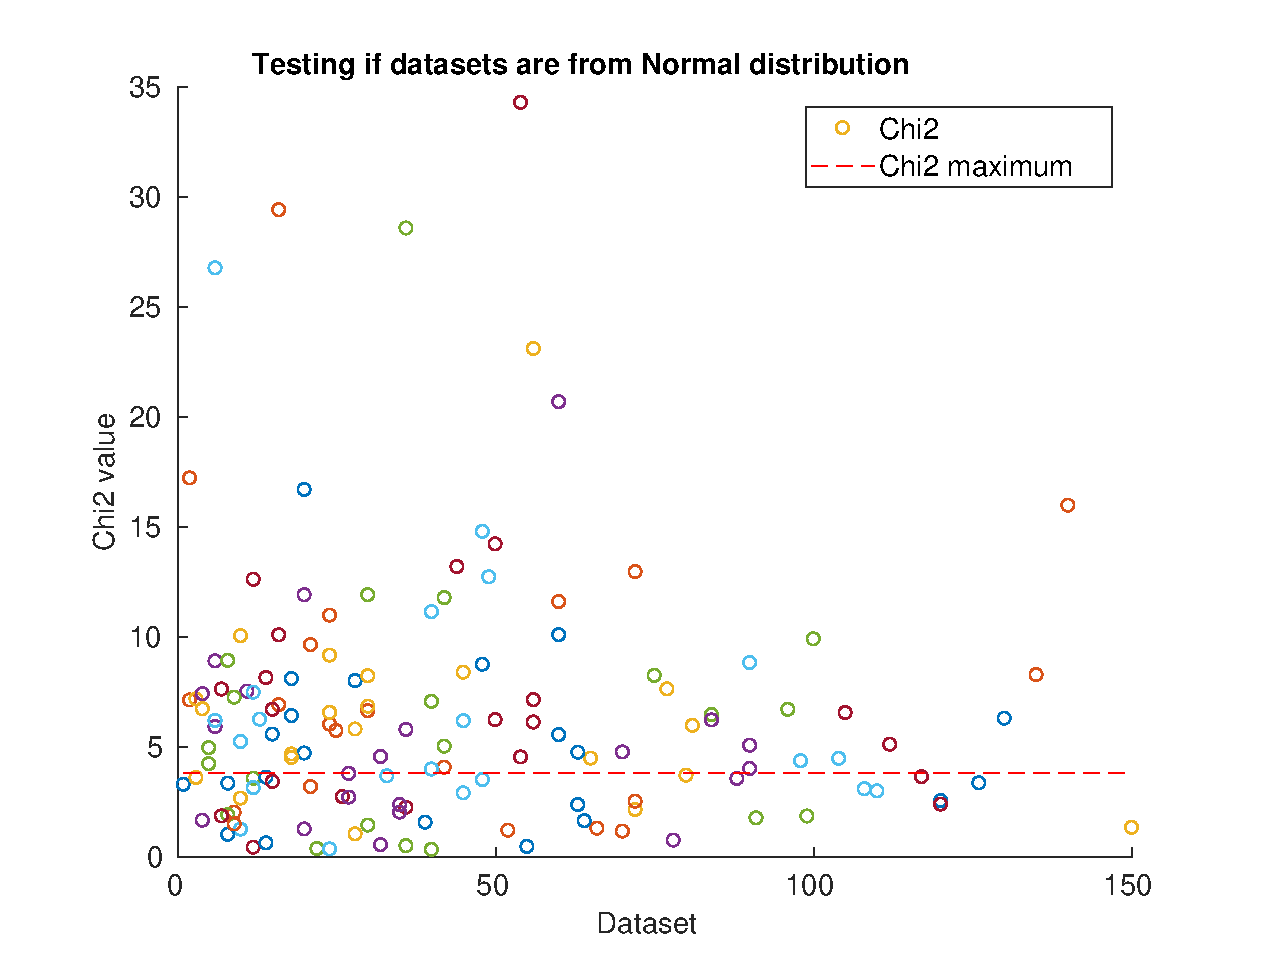
\includegraphics[width=1\columnwidth]{Ex2/ChiDistr.eps}	
\caption{Αποτελέσματα $\chi^{2}$ για κάθε δραστηριότητα και χώρα καθώς και το μέγιστο όριο με διακεκομμένη γραμμή.}
\label{fig:z21} 
\end{figure}

Από το \hyperref[fig:z21]{σχήμα \ref*{fig:z21}} παρατηρούμε ότι αρκετά 
$\chi^{2}$ βρίσκονται επάνω από το μέγιστο $\chi^{2}_{1-\alpha,n-3}$. Για τους βαθμούς ελευθερίας χρησιμοποιούμε $n-3$ γιατί συγκρίνουμε με την συνεχή κανονική κατανομή που έχει δύο ακόμα δεσμευτικές παραμέτρους, την μέση τιμή και την απόκλιση.


Το πρόγραμμα επίσης μας επιστρέφει αν βρήκε μια κατανομή να είναι κανονική ή όχι με βάση κάποιο όριο πιθανότητας. Παρακάτω είναι τα αποτελέσματα αυτού του ελέγχου.

\begin{Verbatim}[fontsize=\small]
At the significance level of  5.00% the percentage of the datasets
that could be from a Normal distribution are 37.33% 

At the confindence level of  5.00%

Does Agriculture Follow a normal distribution : YES
Does EnergyIndustries Follow a normal distribution : YES
Does EnergyIndustriesPowerProduction1A1a Follow a normal distribution : NO
Does FugitiveEmissions Follow a normal distribution : NO
Does IndustryEnergy Follow a normal distribution : NO
Does IndustryProcesses Follow a normal distribution : YES
Does OtherEnergy Follow a normal distribution : YES
Does OtherTransport Follow a normal distribution : NO
Does RoadTransport Follow a normal distribution : NO
Does Waste Follow a normal distribution : NO
\end{Verbatim}

Παρατηρούμε ότι στο επίπεδο σημαντικότητας $5\%$ περίπου το $37\%$ από όλα τα σετ θα μπορούσε να θεωρηθεί ότι προέρχεται από κανονική κατανομή. Επίσης στο ίδιο ποσοστό σημαντικότητας βλέπουμε ότι μόνο 4 στις 10 δραστηριότητες θα μπορούσαν να προέρχονται από κανονική κατανομή.

\begin{figure}[H]

	\centering
	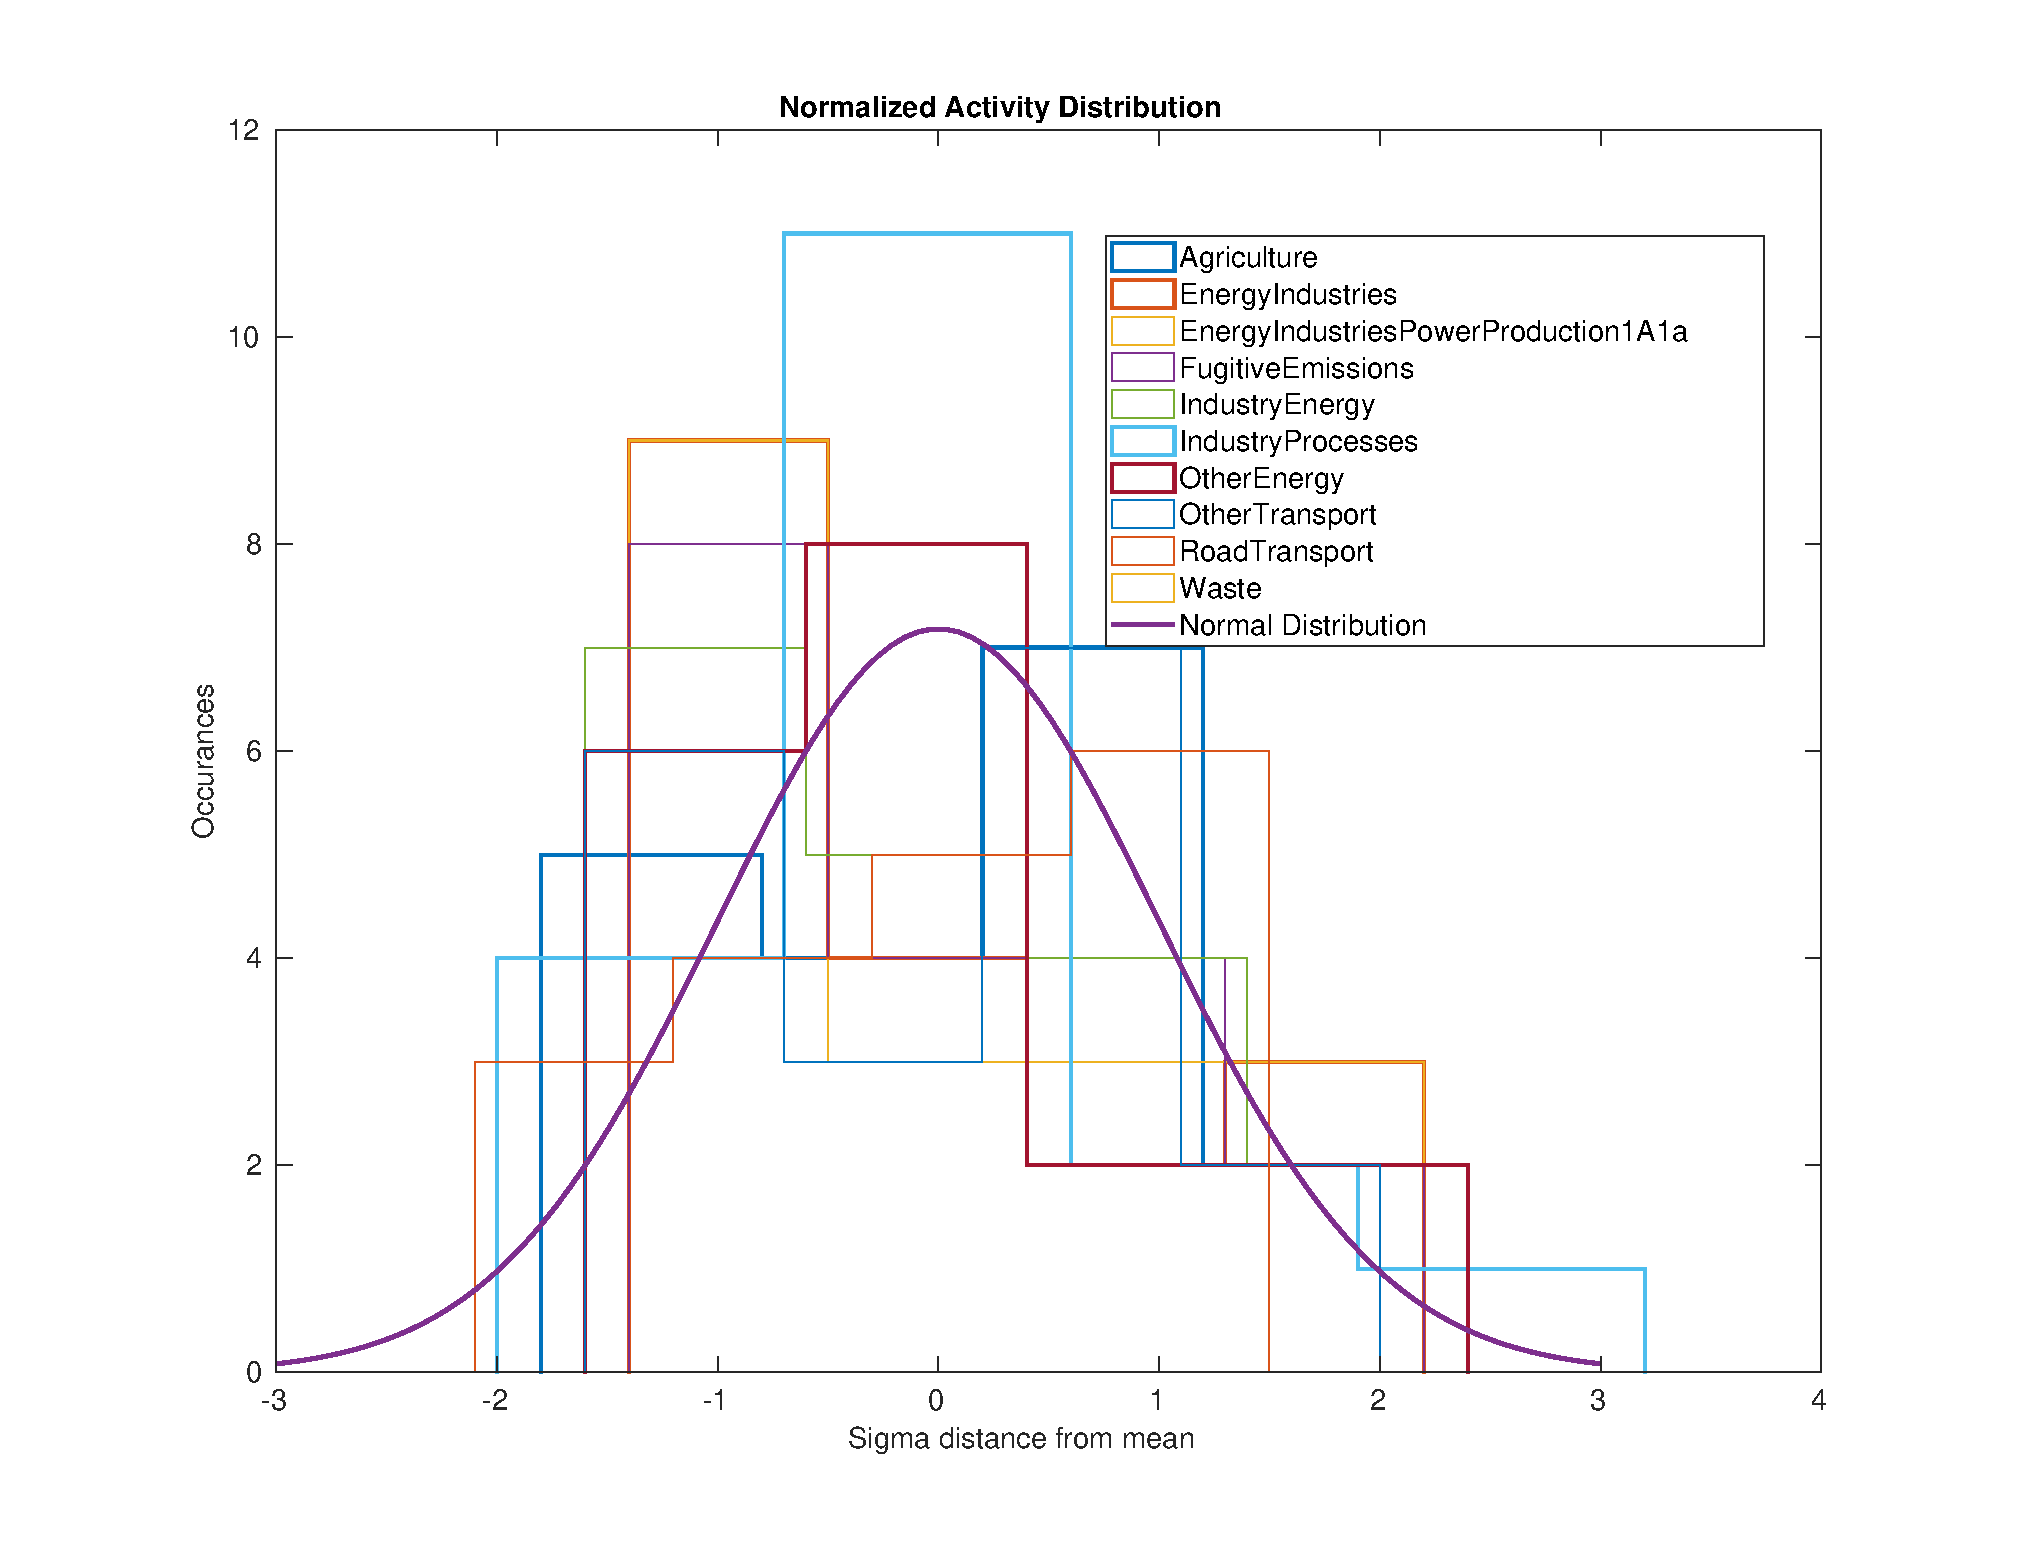
\includegraphics[width=1\columnwidth]{Ex2/ActDistr.eps}	
\caption{Κανονικοποιημένες συνολικές κατανομές για όλες τις δραστηριότητες καθώς και ενδεικτική κανονική κατανομή για σύγκριση. Οι δραστηριότητες με ποιο έντονη γραμμή έχουν περάσει το τεστ κανονικότητας.}
\label{fig:z22} 
\end{figure}

Στο \hyperref[fig:z22]{σχήμα \ref*{fig:z22}} παρατηρούμε ότι γενικά οι κανονικοποιημένες κατανομές των δραστηριοτήτων διαφέρουν από κανονικές. Πέρα απο τα αποτελέσματα που μας επιστρέφει το πρόγραμμα θα μπορούσε κάποιος οπτικά και μόνο να πει ότι από όλες τις κατανομές αυτές που φαίνεται να ακολουθούν κανονική κατανομή είναι: IndustryProcesses και OtherEnergy.   






\subsection{Ζήτημα 3}
\label{subsec:z3}

Για την επίλυση αυτού του ζητήματος κάνουμε χρήση του \hyperref[mat:3]{κώδικα \ref*{mat:3}}. Ενδεικτικά εκτελέσαμε τον κώδικα για 4 δραστηριότητες και τα αποτελέσματα φαίνονται στα \hyperref[fig:z31]{σχήμα \ref*{fig:z31}},\hyperref[fig:z32]{σχήμα \ref*{fig:z32}},\hyperref[fig:z33]{σχήμα \ref*{fig:z33}} και \hyperref[fig:z34]{σχήμα \ref*{fig:z34}}.


\begin{figure}[H]

	\centering
	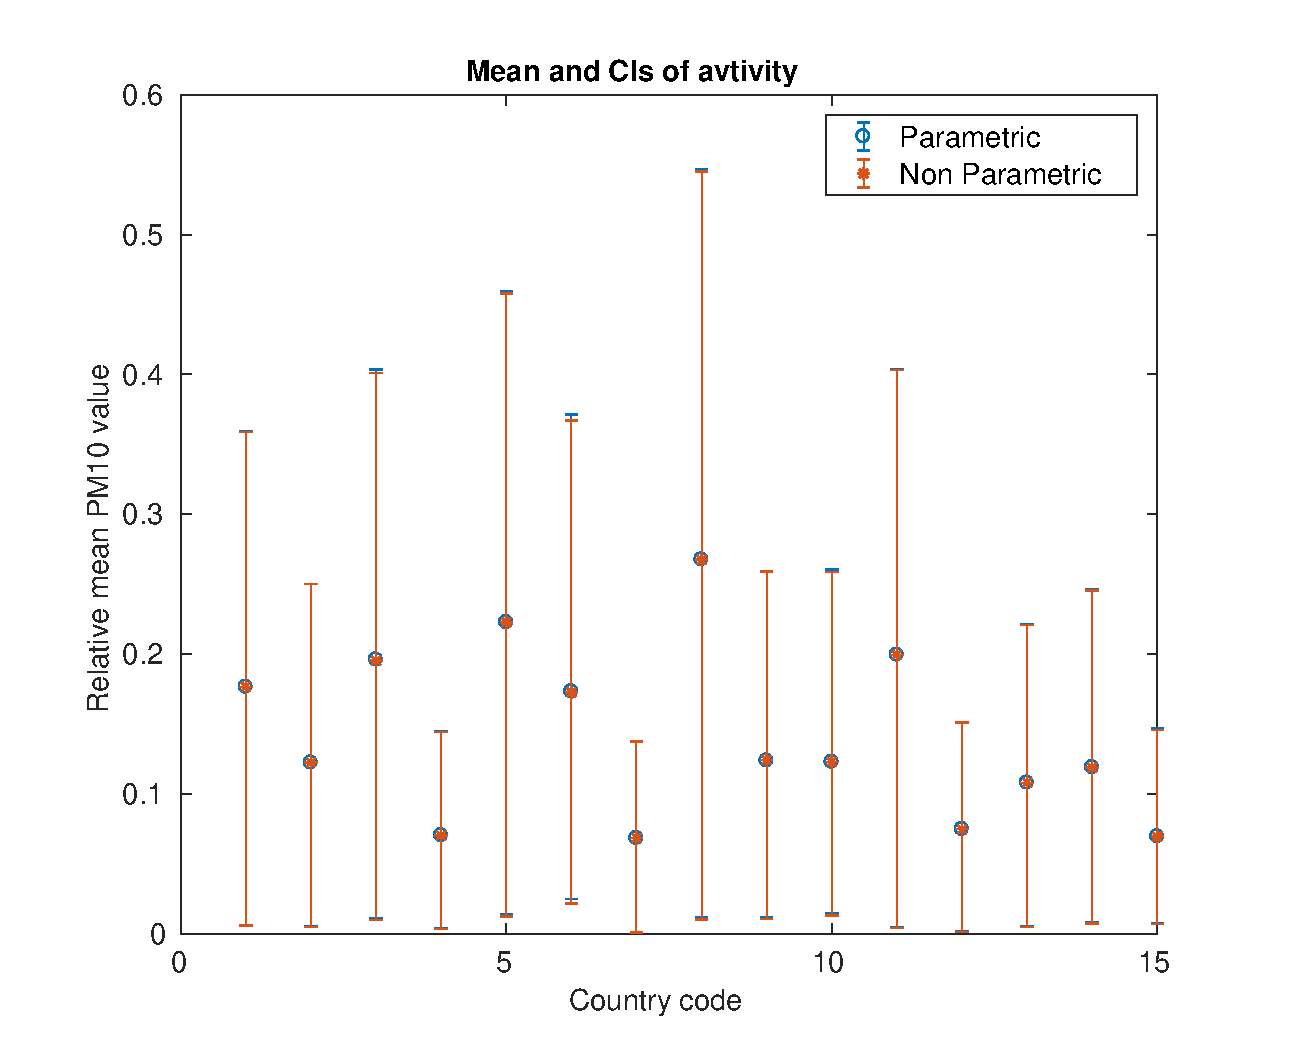
\includegraphics[width=1\columnwidth]{Ex3/Agriculture.eps}	
\caption{Μέσες τιμές και παραμετρικά και μη παραμετρικά διαστήματα για την δραστηριότητα Agriculture σε κάθε χώρα.}
\label{fig:z31} 
\end{figure}

\begin{figure}[H]
 
	\centering
	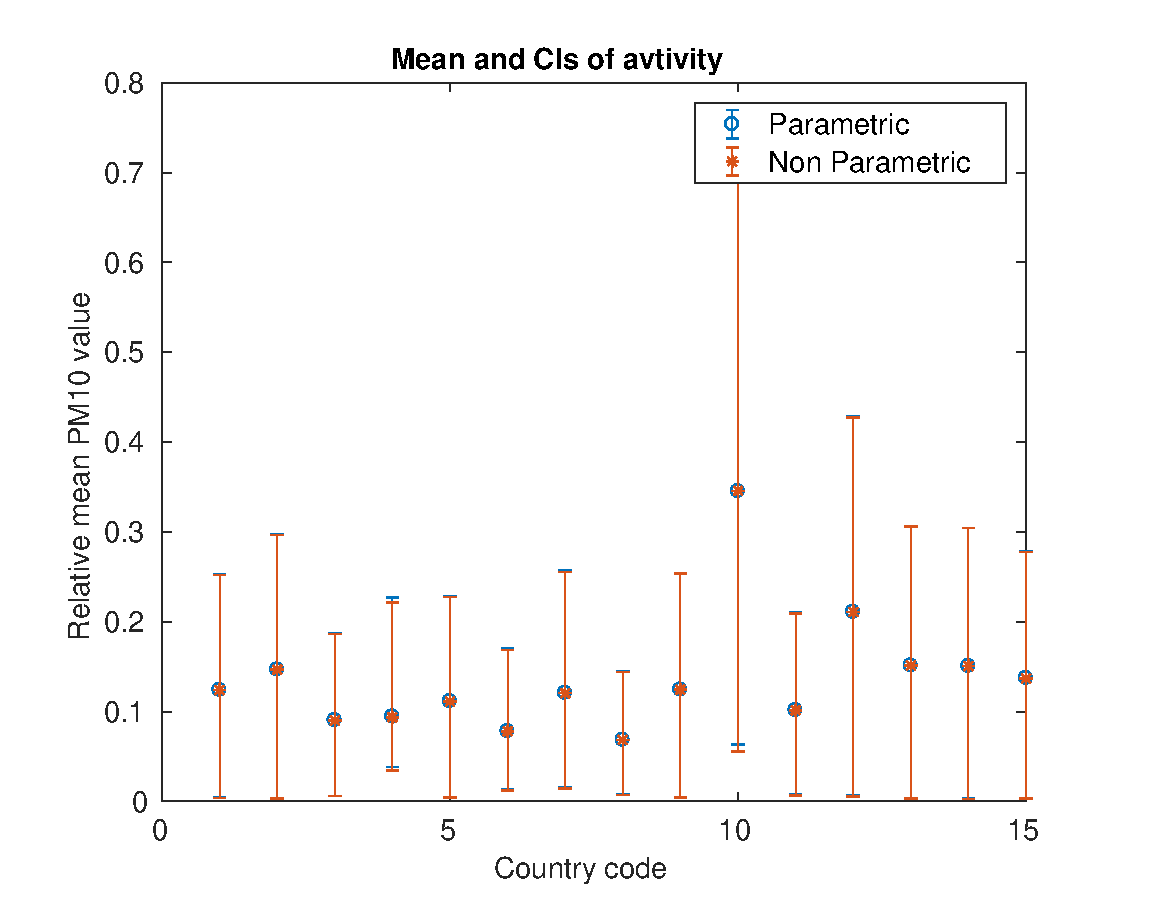
\includegraphics[width=1\columnwidth]{Ex3/IndustryEnergy.eps}	
\caption{Μέσες τιμές και παραμετρικά και μη παραμετρικά διαστήματα για την δραστηριότητα IndustryEnergy σε κάθε χώρα.}
\label{fig:z32}
\end{figure}

\begin{figure}[H]

	\centering
	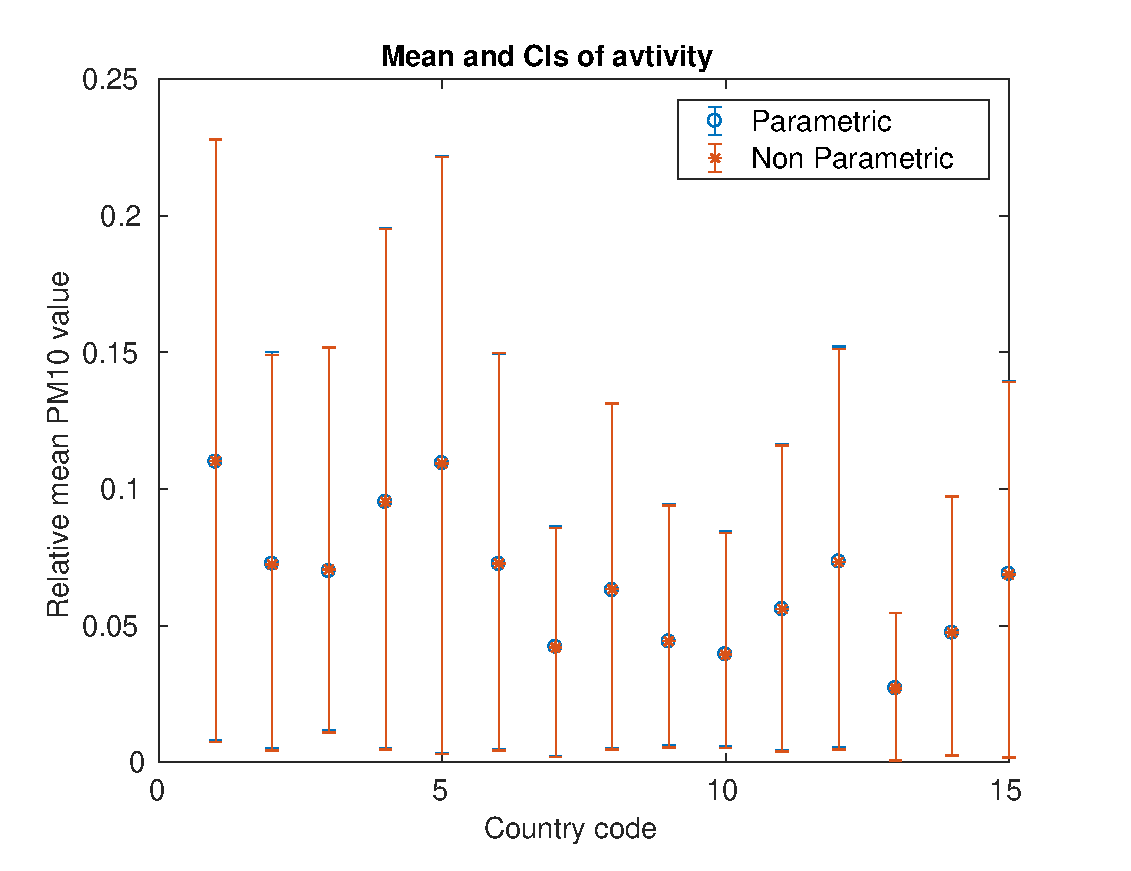
\includegraphics[width=1\columnwidth]{Ex3/OtherEnergy.eps}	
\caption{Μέσες τιμές και παραμετρικά και μη παραμετρικά διαστήματα για την δραστηριότητα OtherEnergy σε κάθε χώρα.}
\label{fig:z33} 
\end{figure}

\begin{figure}[H]
 
	\centering
	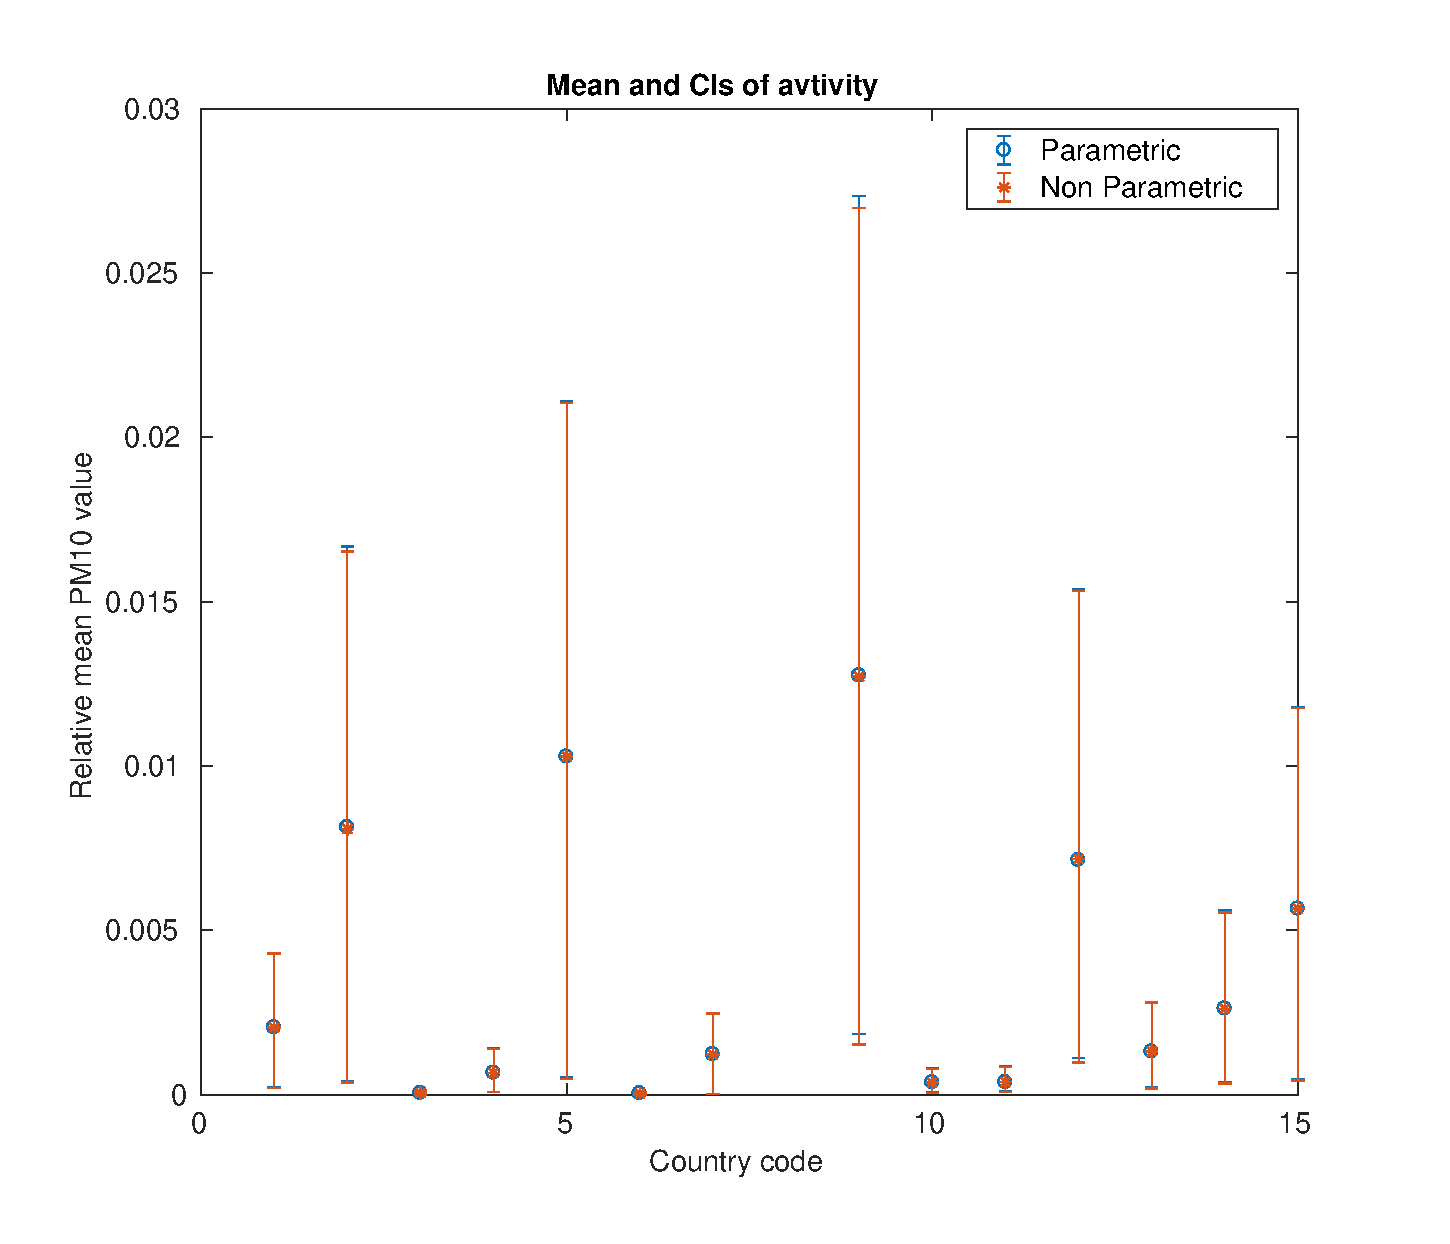
\includegraphics[width=1\columnwidth]{Ex3/Waste.eps}	
\caption{Μέσες τιμές και παραμετρικά και μη παραμετρικά διαστήματα για την δραστηριότητα Waste σε κάθε χώρα.}
\label{fig:z34}
\end{figure}


Από τα παραπάνω σχήματα δεν φαίνεται να υπάρχει μεγάλη διαφορά μεταξύ των μέσων τιμών και των διαστημάτων εμπιστοσύνης που προέρχονται από παραμετρική και με παραμετρική εκτίμηση.

\subsection{Ζήτημα 4}
\label{subsec:z4}

Η ίδια ανάλυση όπως και στο \hyperref[subsec:z3]{Κεφάλαιο \ref*{subsec:z3}} αλλά τώρα για την τυπική απόκλιση. Η ανάλυση γίνεται με τον \hyperref[mat:4]{κώδικα \ref*{mat:4}}. Καλέσαμε τον παραπάνω κώδιακ ενδεικτικά για μερικές δραστηριότητες και πήραμε τα παρακάτω \hyperref[fig:z41]{σχήμα \ref*{fig:z41}},\hyperref[fig:z42]{σχήμα \ref*{fig:z42}},\hyperref[fig:z43]{σχήμα \ref*{fig:z43}} και \hyperref[fig:z44]{σχήμα \ref*{fig:z44}}.

\begin{figure}[H]

	\centering
	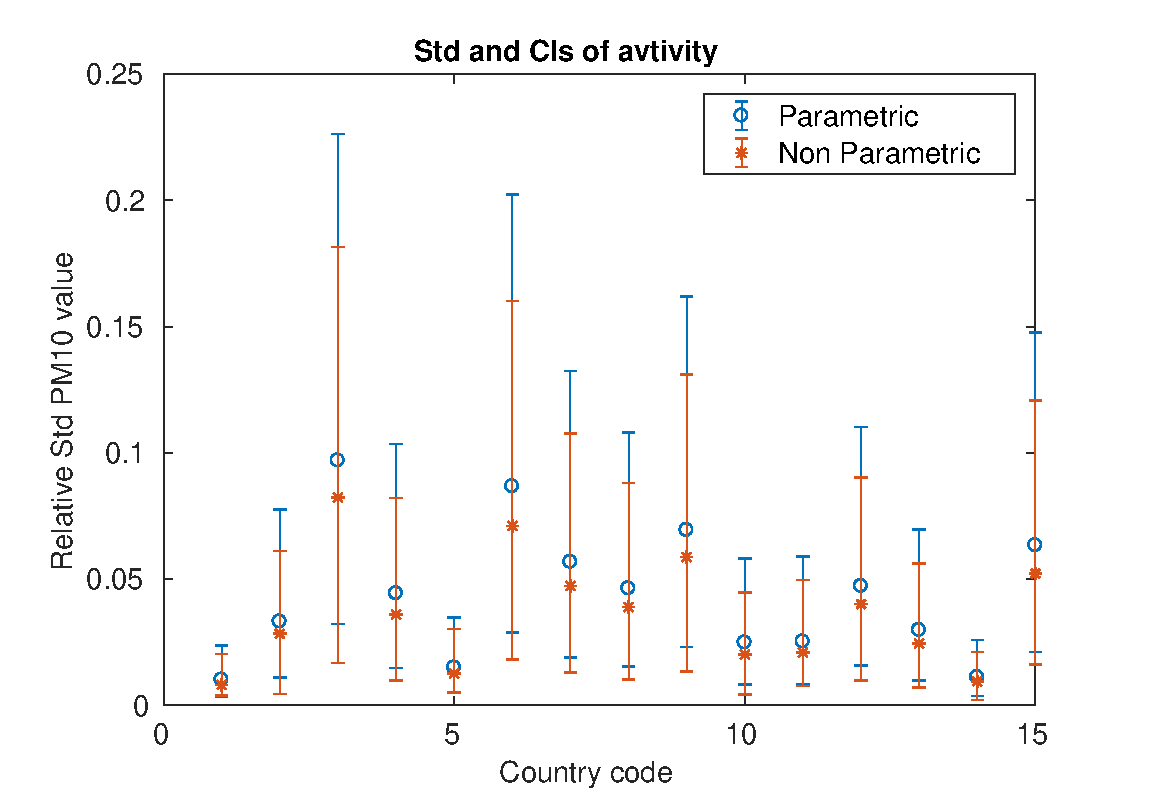
\includegraphics[width=1\columnwidth]{Ex4/EnergyIndustries.eps}	
\caption{Μέσες τιμές και παραμετρικά και μη παραμετρικά διαστήματα της τυπικής απόκλισης για την δραστηριότητα EnergyIndustries σε κάθε χώρα.}
\label{fig:z41} 
\end{figure}

\begin{figure}[H]

	\centering
	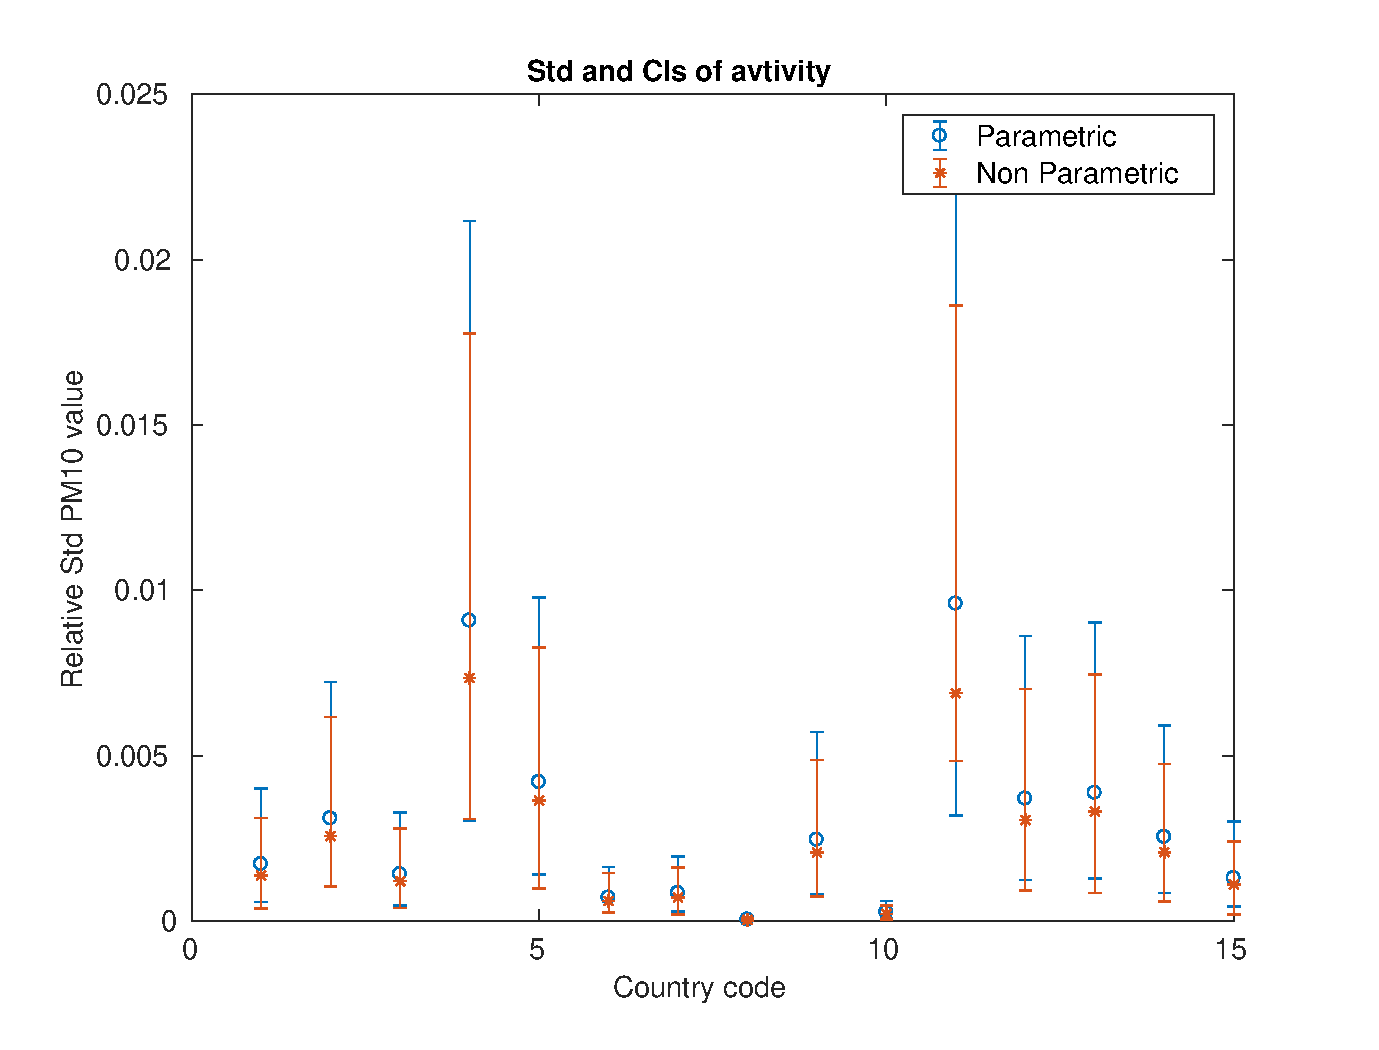
\includegraphics[width=1\columnwidth]{Ex4/FugitiveEmissions.eps}	
\caption{Μέσες τιμές και παραμετρικά και μη παραμετρικά διαστήματα της τυπικής απόκλισης για την δραστηριότητα FugitiveEmissions σε κάθε χώρα.}
\label{fig:z42} 
\end{figure}

\begin{figure}[H]
 
	\centering
	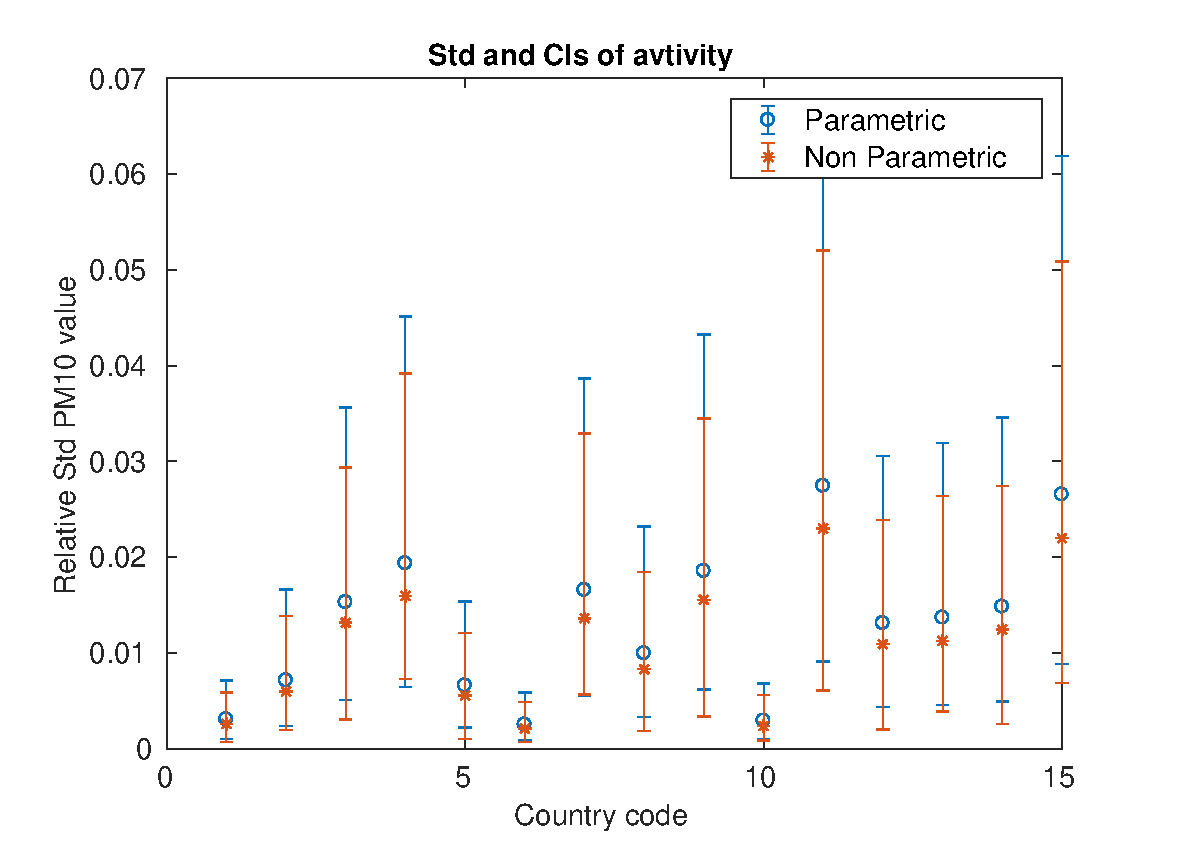
\includegraphics[width=1\columnwidth]{Ex4/OtherTransport.eps}	
\caption{Μέσες τιμές και παραμετρικά και μη παραμετρικά διαστήματα της τυπικής απόκλισης για την δραστηριότητα Othertransport σε κάθε χώρα.}
\label{fig:z43}
\end{figure}

\begin{figure}[H]

	\centering
	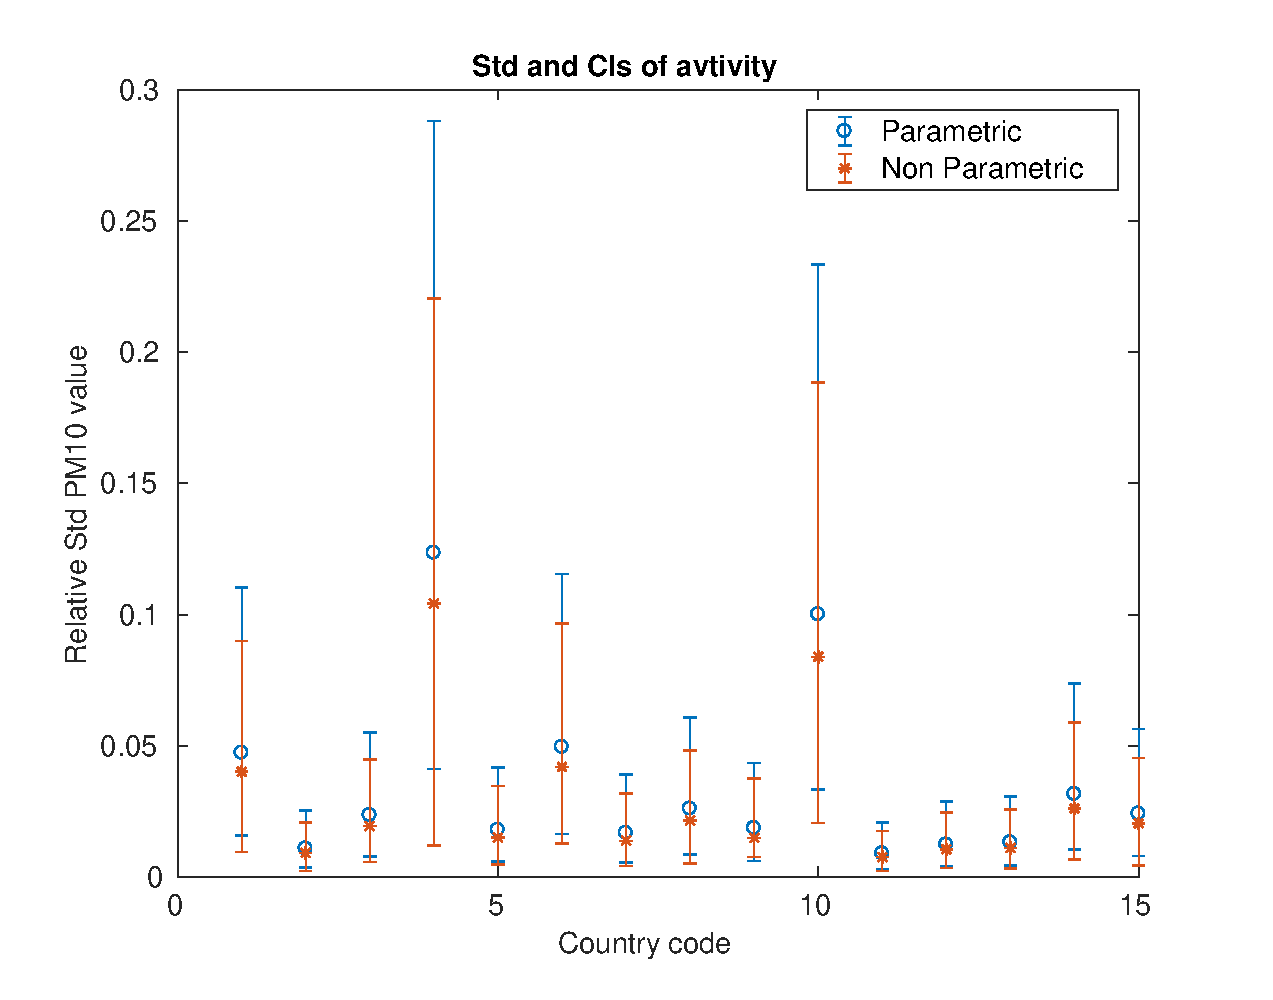
\includegraphics[width=1\columnwidth]{Ex4/RoadTransport.eps}	
\caption{Μέσες τιμές και παραμετρικά και μη παραμετρικά διαστήματα της τυπικής απόκλισης για την δραστηριότητα RoadTransport σε κάθε χώρα.}
\label{fig:z44} 
\end{figure}

Από τα παραπάνω σχήματα παρατηρούμε ότι η μέσες τιμές της τυπικής απόκλισης διαφέρουν ανάμεσα στον παραμετρικό και μη τρόπο υπολογισμού τους. Καθώς και ότι σε γενικές γραμμές τα μη παραμετρικά διαστήματα εμπιστοσύνης είναι μικρότερα από τα αντίστοιχα παραμετρικά. Αυτό μπορεί να οφείλεται στον μεγάλο αριθμό (1000) τυχαίων δειγμάτων που δημιουργήσαμε στην μη παραμετρική ανάλυσή μας.  

\subsection{Ζήτημα 5}
\label{subsec:z5}

Για την επίλυση αυτού του ζητήματος κάνουμε χρήση του \hyperref[mat:5]{κώδικα \ref*{mat:5}}. Κατά την διάρκεια εκτέλεσης του κώδικα το Matlab επιστρέφει ένα γράφημα και τα αποτελέσματα του τεστ στην οθόνη. Ενδεικτικά καλέσαμε τον παραπάνω κώδικα για 4 δραστηριότητες και τα αποτελέσματα είναι παρακάτω. Στα αποτελέσματα που εκτυπώνονται αναφέρεται η απόλυτη τιμή του συντελεστή συσχέτισης.




\begin{figure}[H]

	\centering
	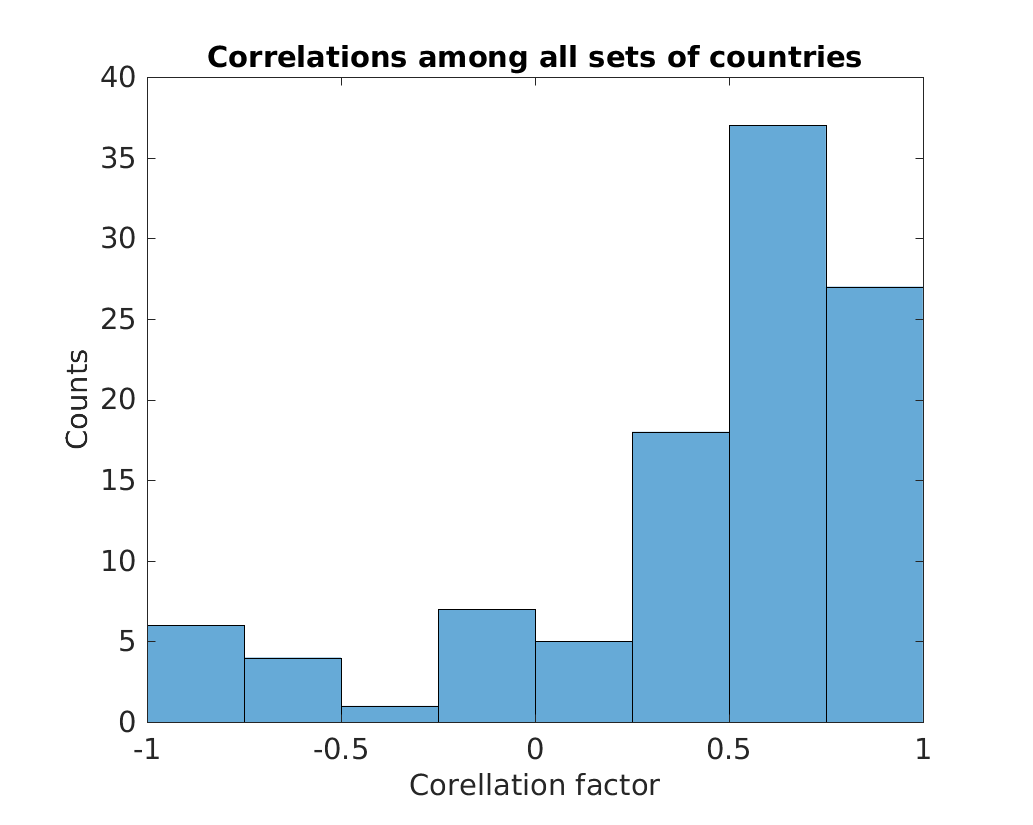
\includegraphics[width=1\columnwidth]{Ex5/Agriculture.eps}	
\caption{Ιστόγραμμα των συντελεστών συσχέτισης της δραστηριότητας Agriculture.}
\label{fig:z51} 
\end{figure}



\begin{Verbatim}[fontsize=\small]
The 10 sets of countries with the highest 
correlation for Agriculture are
Correlation	 Country1	 Country2
 0.98	 	    Denmark	      Italy 
 0.97	 	 Netherlands	 United Kingdom 
 0.95	 	    Denmark	 Netherlands 
 0.95	 	      Italy	 United Kingdom 
 0.94	 	      Italy	 Netherlands 
 0.94	 	    Austria	    Belgium 
 0.94	 	    Denmark	 United Kingdom 
 0.91	 	    Belgium	 United Kingdom 
 0.91	 	    Austria	 Luxembourg 
 0.91	 	    Austria	 United Kingdom 

 29.52% of the sets of countries pass 
the Parametric test with a significance level of  5.00%

 24.76% of the sets of countries pass 
the NON-Parametric test with a significance level of  5.00%
\end{Verbatim}



\begin{figure}[H]
 
	\centering
	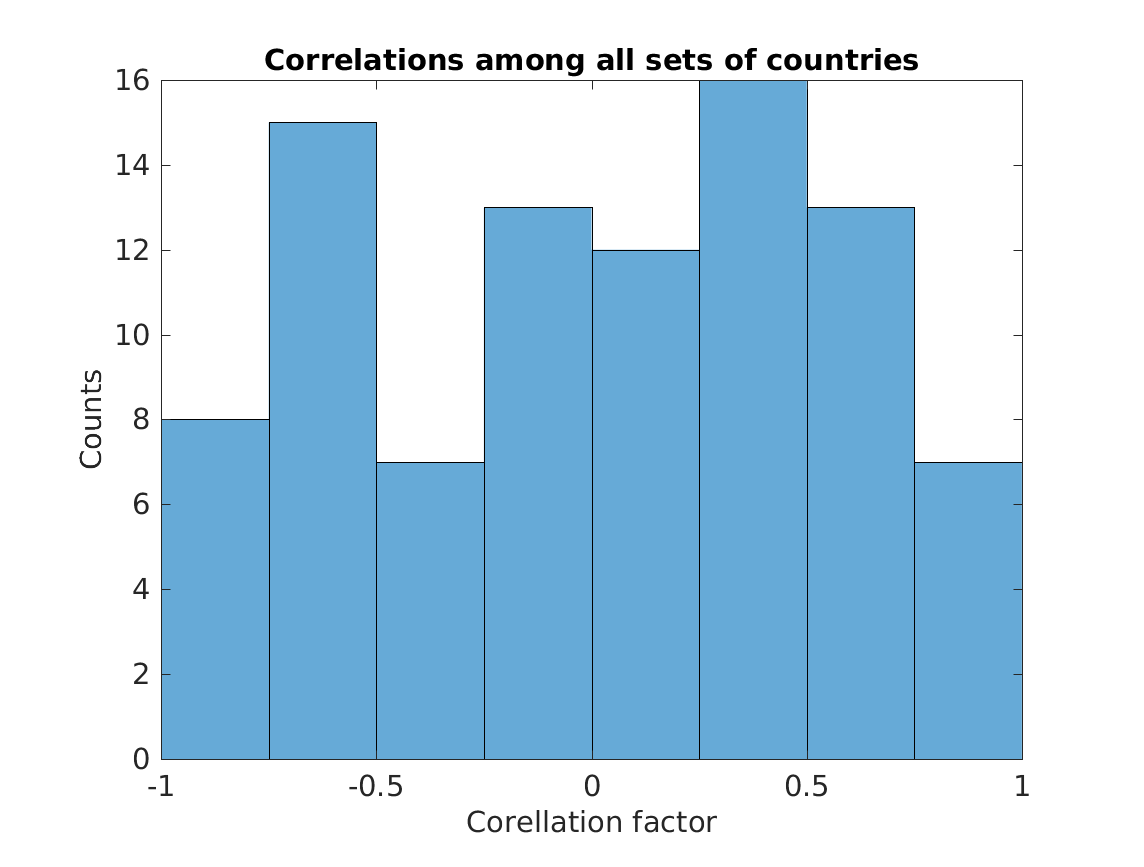
\includegraphics[width=1\columnwidth]{Ex5/Waste.eps}	
\caption{Ιστόγραμμα των συντελεστών συσχέτισης της δραστηριότητας Waste.}
\label{fig:z52}
\end{figure}



\begin{Verbatim}[fontsize=\small]
The 10 sets of countries with the highest 
correlation for Waste are
Correlation	 Country1	 Country2
 0.88	 	    Germany	 Luxembourg 
 0.87	 	    Austria	    Germany 
 0.87	 	     Sweden	 United Kingdom 
 0.86	 	   Portugal	     Sweden 
 0.86	 	    Austria	 Luxembourg 
 0.86	 	   Portugal	 United Kingdom 
 0.85	 	 Luxembourg	 United Kingdom 
 0.83	 	 Netherlands	   Portugal 
 0.82	 	    Germany	      Spain 
 0.82	 	 Luxembourg	   Portugal 

 44.76% of the sets of countries pass 
the Parametric test with a significance level of  5.00%

 58.10% of the sets of countries pass 
the NON-Parametric test with a significance level of  5.00%
\end{Verbatim}




\begin{figure}[H]

	\centering
	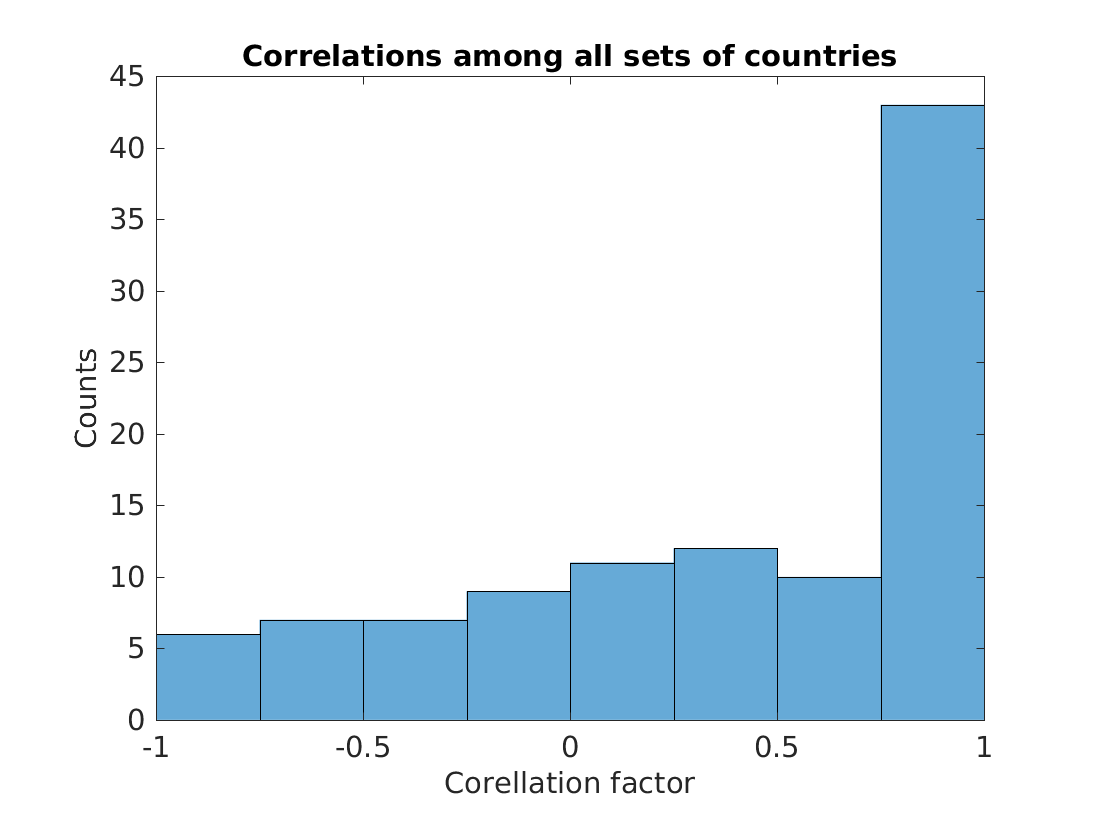
\includegraphics[width=1\columnwidth]{Ex5/IndustryEnergy.eps}	
\caption{Ιστόγραμμα των συντελεστών συσχέτισης της δραστηριότητας IndustryEnergy.}
\label{fig:z53} 
\end{figure}



\begin{Verbatim}[fontsize=\small]
The 10 sets of countries with the highest 
correlation for IndustryEnergy are
Correlation	 Country1	 Country2
 0.99	 	     France	      Italy 
 0.98	 	 Luxembourg	 United Kingdom 
 0.97	 	      Italy	 Luxembourg 
 0.97	 	     France	 United Kingdom 
 0.97	 	    Belgium	 United Kingdom 
 0.97	 	      Italy	 United Kingdom 
 0.97	 	     France	 Luxembourg 
 0.97	 	     Sweden	 United Kingdom 
 0.96	 	    Belgium	      Italy 
 0.96	 	     France	     Sweden 

 35.24% of the sets of countries pass 
the Parametric test with a significance level of  5.00%

 35.24% of the sets of countries pass 
the NON-Parametric test with a significance level of  5.00%
\end{Verbatim}


\begin{figure}[H]

	\centering
	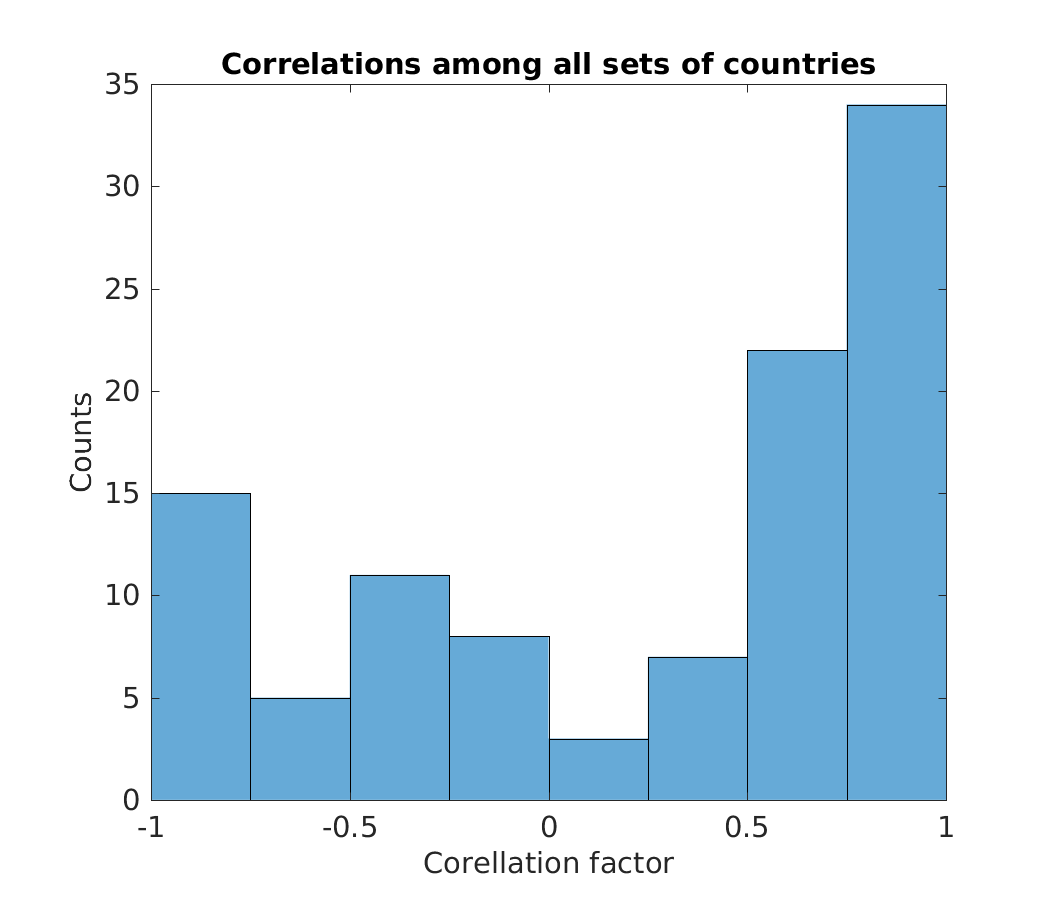
\includegraphics[width=1\columnwidth]{Ex5/RoadTransport.eps}	
\caption{Ιστόγραμμα των συντελεστών συσχέτισης της δραστηριότητας RoadTransport.}
\label{fig:z54} 
\end{figure}



\begin{Verbatim}[fontsize=\small]
The 10 sets of countries with the highest 
correlation for RoadTransport are
Correlation	 Country1	 Country2
 1.00	 	    Denmark	 United Kingdom 
 0.99	 	    Denmark	     France 
 0.99	 	    Belgium	     France 
 0.99	 	    Denmark	     Sweden 
 0.99	 	    Germany	 United Kingdom 
 0.99	 	     France	 United Kingdom 
 0.99	 	     France	      Italy 
 0.99	 	     Sweden	 United Kingdom 
 0.99	 	     France	     Sweden 
 0.99	 	    Denmark	      Italy 

 25.71% of the sets of countries pass 
the Parametric test with a significance level of  5.00%

 26.67% of the sets of countries pass 
the NON-Parametric test with a significance level of  5.00%
\end{Verbatim}











\subsection{Ζήτημα 6}
\label{subsec:z6}

Για την επίλυση αυτού του ζητήματος κάνουμε χρήση του \hyperref[mat:6]{κώδικα \ref*{mat:6}}.

\begin{figure}[H]

	\centering
	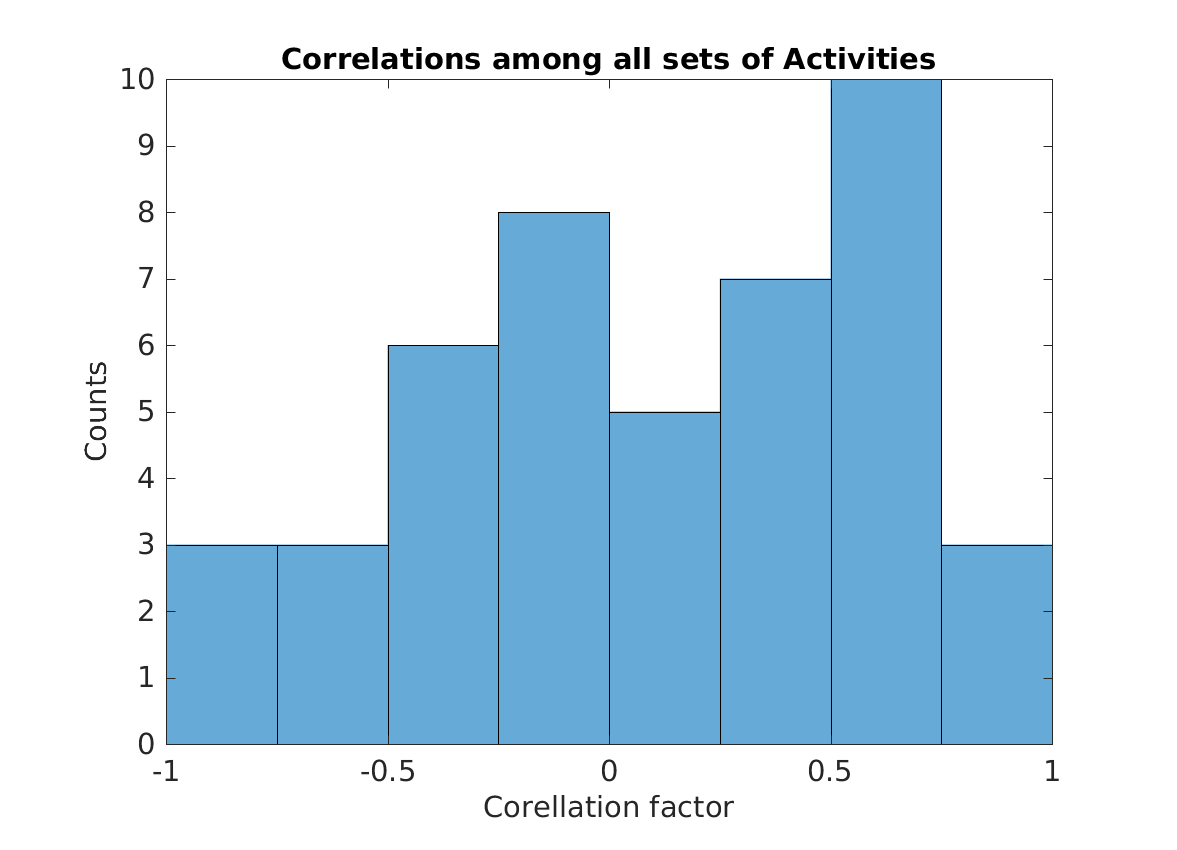
\includegraphics[width=1\columnwidth]{Ex6/Austria.eps}	
\caption{Ιστόγραμμα των συντελεστών συσχέτισης για την Austria.}
\label{fig:z61} 
\end{figure}



\begin{Verbatim}[fontsize=\small]
The 10 sets of Activities with the highest correlation for Austria are
Correlation	 Activity1	 	 Activity2
 1.00	     EnergyIndustries	 	 EnergyIndustriesPowerProduction1A1a 
 0.91	          Agriculture	 	        RoadTransport 
 0.82	    FugitiveEmissions	 	          OtherEnergy 
 0.82	          Agriculture	 	                Waste 
 0.79	          OtherEnergy	 	                Waste 
 0.76	        RoadTransport	 	                Waste 
 0.75	 EnergyIndustriesPowerProduction1A1a	 	       IndustryEnergy 
 0.74	 EnergyIndustriesPowerProduction1A1a	 	    IndustryProcesses 
 0.74	     EnergyIndustries	 	    IndustryProcesses 
 0.72	     EnergyIndustries	 	       IndustryEnergy 

 53.33% of the sets of Activities pass 
the Parametric test with a significance level of  5.00%

 51.11% of the sets of Activities pass 
the NON-Parametric test with a significance level of  5.00%
\end{Verbatim}


\begin{figure}[H]
 
	\centering
	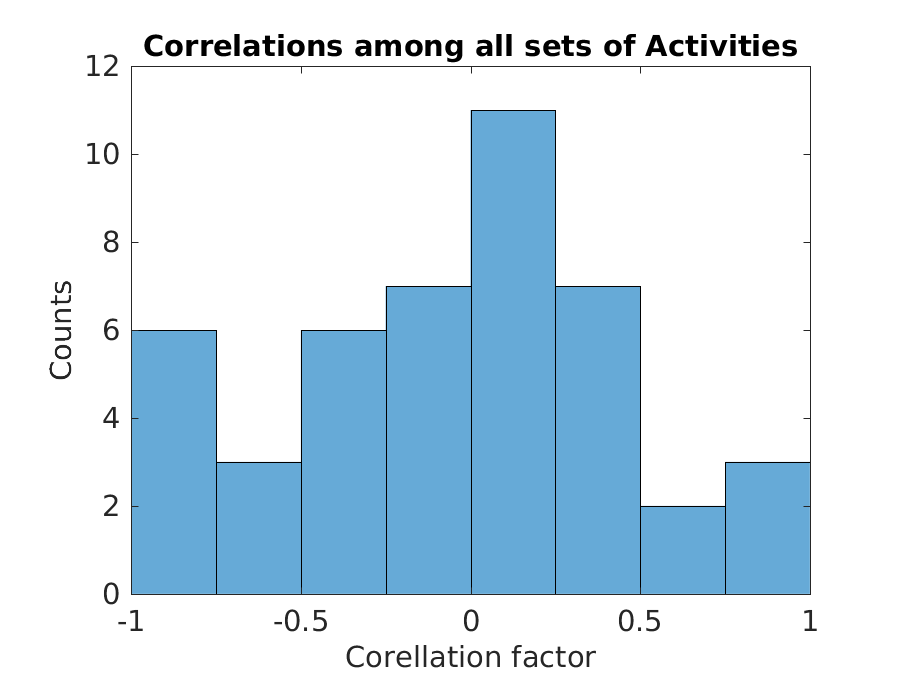
\includegraphics[width=1\columnwidth]{Ex6/Spain.eps}	
\caption{Ιστόγραμμα των συντελεστών συσχέτισης για την Spain.}
\label{fig:z62}
\end{figure}



\begin{Verbatim}[fontsize=\small]
The 10 sets of Activities with the highest correlation for Spain are
Correlation	 Activity1	 	 Activity2
 0.99	     EnergyIndustries	 	 EnergyIndustriesPowerProduction1A1a 
 0.92	       OtherTransport	 	                Waste 
 0.88	        RoadTransport	 	                Waste 
 0.86	    FugitiveEmissions	 	       OtherTransport 
 0.83	       OtherTransport	 	        RoadTransport 
 0.81	    FugitiveEmissions	 	                Waste 
 0.79	          Agriculture	 	     EnergyIndustries 
 0.79	          Agriculture	 	    FugitiveEmissions 
 0.77	    FugitiveEmissions	 	        RoadTransport 
 0.74	          Agriculture	 	 EnergyIndustriesPowerProduction1A1a 

 64.44% of the sets of Activities pass 
the Parametric test with a significance level of  5.00%

 66.67% of the sets of Activities pass 
the NON-Parametric test with a significance level of  5.00%
\end{Verbatim}


\begin{figure}[H]

	\centering
	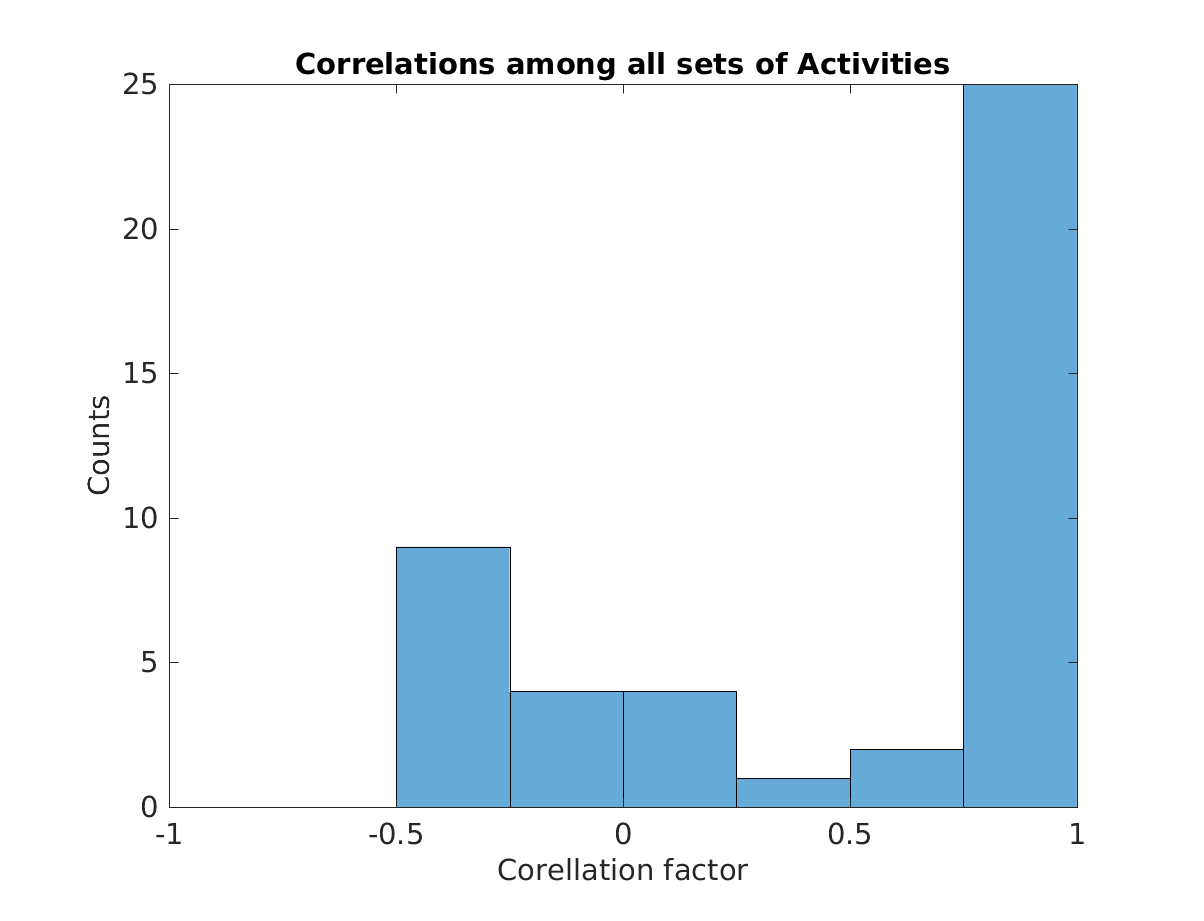
\includegraphics[width=1\columnwidth]{Ex6/Italy.eps}	
\caption{Ιστόγραμμα των συντελεστών συσχέτισης για την Italy.}
\label{fig:z63} 
\end{figure}



\begin{Verbatim}[fontsize=\small]
The 10 sets of Activities with the highest correlation for Italy are
Correlation	 Activity1	 	 Activity2
 1.00	     EnergyIndustries	 	 EnergyIndustriesPowerProduction1A1a 
 0.97	     EnergyIndustries	 	        RoadTransport 
 0.96	 EnergyIndustriesPowerProduction1A1a	 	        RoadTransport 
 0.96	     EnergyIndustries	 	       IndustryEnergy 
 0.96	 EnergyIndustriesPowerProduction1A1a	 	       IndustryEnergy 
 0.95	          Agriculture	 	     EnergyIndustries 
 0.95	          Agriculture	 	 EnergyIndustriesPowerProduction1A1a 
 0.93	          Agriculture	 	        RoadTransport 
 0.92	          Agriculture	 	       IndustryEnergy 
 0.91	       IndustryEnergy	 	        RoadTransport 

 40.00% of the sets of Activities pass 
the Parametric test with a significance level of  5.00%

 37.78% of the sets of Activities pass 
the NON-Parametric test with a significance level of  5.00%
\end{Verbatim}



\begin{figure}[H]

	\centering
	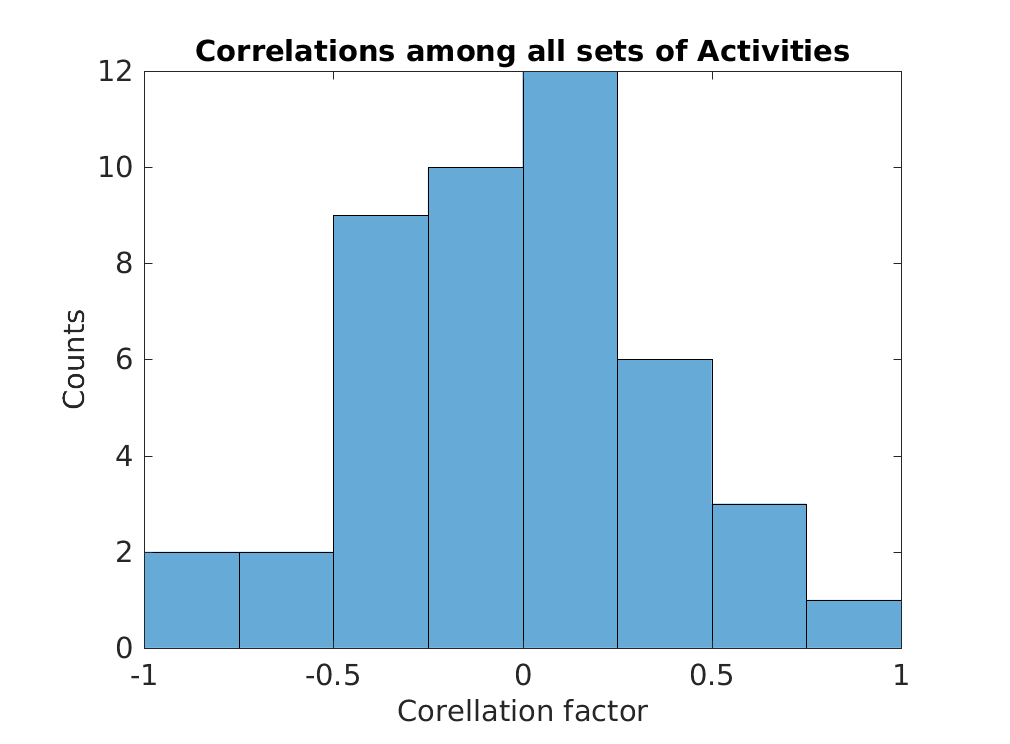
\includegraphics[width=1\columnwidth]{Ex6/Greece.eps}	
\caption{Ιστόγραμμα των συντελεστών συσχέτισης για την Greece.}
\label{fig:z64} 
\end{figure}



\begin{Verbatim}[fontsize=\small]

The 10 sets of Activities with the highest correlation for Greece are
Correlation	 Activity1	 	 Activity2
 1.00	     EnergyIndustries	 	 EnergyIndustriesPowerProduction1A1a 
 0.92	 EnergyIndustriesPowerProduction1A1a	 	       IndustryEnergy 
 0.92	     EnergyIndustries	 	       IndustryEnergy 
 0.66	     EnergyIndustries	 	        RoadTransport 
 0.65	       IndustryEnergy	 	    IndustryProcesses 
 0.62	 EnergyIndustriesPowerProduction1A1a	 	        RoadTransport 
 0.59	          Agriculture	 	       IndustryEnergy 
 0.54	          Agriculture	 	    IndustryProcesses 
 0.49	       IndustryEnergy	 	        RoadTransport 
 0.47	          Agriculture	 	 EnergyIndustriesPowerProduction1A1a 

 77.78% of the sets of Activities pass 
the Parametric test with a significance level of  5.00%

 77.78% of the sets of Activities pass 
the NON-Parametric test with a significance level of  5.00%
\end{Verbatim}






\subsection{Ζήτημα 7}
\label{subsec:z7}

Για την επίλυση αυτού του ζητήματος κάνουμε χρήση του \hyperref[mat:7]{κώδικα \ref*{mat:7}}.


\begin{figure}[H]
 
	\centering
	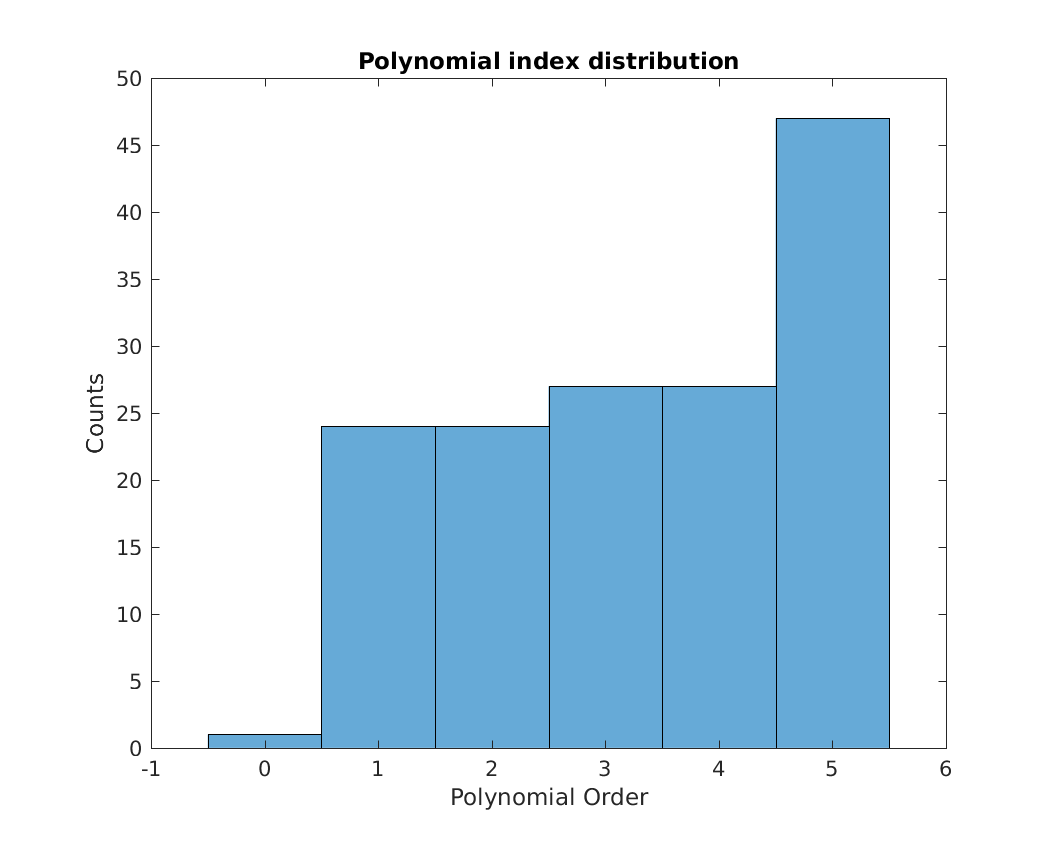
\includegraphics[width=1\columnwidth]{Ex7/PolyDist.eps}	
\caption{Ιστόγραμμα των πολυωνυμικών όρων με το μεγαλύτερο $AdjR^2$.}
\label{fig:z7}
\end{figure}


\begin{Verbatim}[fontsize=\small]
                                            AdjR2     Order        Country     
                                           _______    _____    ________________

    Agriculture                            0.96671    5        'Netherlands'   
    EnergyIndustries                       0.99606    5        'Italy'         
    EnergyIndustriesPowerProduction1A1a    0.99382    5        'Italy'         
    FugitiveEmissions                      0.98047    4        'France'        
    IndustryEnergy                         0.99629    4        'Luxembourg'    
    IndustryProcesses                       0.9754    4        'Sweden'        
    OtherEnergy                            0.97918    4        'Germany'       
    OtherTransport                         0.98636    5        'Germany'       
    RoadTransport                          0.99763    3        'United Kingdom'
    Waste                                  0.93096    2        'Luxembourg'
\end{Verbatim}


\subsection{Ζήτημα 8}
\label{subsec:z8}

Για την επίλυση αυτού του ζητήματος κάνουμε χρήση του \hyperref[mat:8]{κώδικα \ref*{mat:8}}. Παρακάτω δίνονται τα σχήματα και τα αποτελέσματα των βηματικών προσαρμόσεων για κάθε χώρα ξεχωριστά. Στα σχήματα υπάρχει οπτική ανάλυση του πόσο καλά προσαρμόζονται οι εκτιμήσεις στα πραγματικά δεδομένα. Ενώ στο επιστρεφόμενο κείμενο από των κώδικα υπάρχει η πληροφορία για το $AdjR^2$ καθώς και τους συντελεστές της κάθε προσαρμογής. Οι κατηγορίες Stepwizefit, MyStepwise και Full αντιστοιχούν στις προσαρμογές που έγιναν με την stepwisefit function του Matlab, την δική μασ συνάρτηση και το πλήρες μοντέλο αντίστοιχα.

Σε γενικές γραμμές οι προσαρμογές αναπαριστούν τα αρχικά δεδομένα με καλή ακρίβεια. Υπάρχουν μερικά προβλήματα όπως στην περίπτωση της Greece και Ireland όπου υπάρχουν κενά στα δεδομένα με αποτέλεσμα να επηρεάζουν την διαδικασία προσαρμογής. 


\begin{figure}[H]

	\centering
	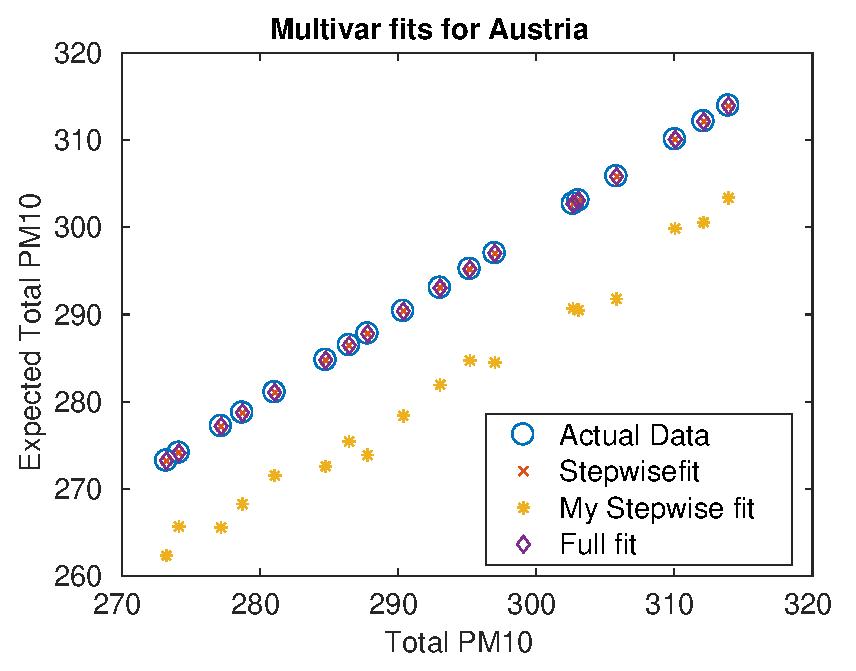
\includegraphics[width=1\columnwidth]{Ex8/Austria_MultivarFits.eps}	
\caption{Πραγματικές και εκτιμούμενες τιμές για την Austria.}
\label{fig:z81} 
\end{figure}

\begin{Verbatim}[fontsize=\small]
Multivariable fitting for Activities in Country
 	 	 Austria

                                           Stepwisefit    MyStepwise       Full    
                                           ___________    __________    ___________

    AdjR2                                        1        0.98418                 1
    Intercept                              0.57636         125.45           0.57587
    Agriculture                            0.99855              0           0.99856
    EnergyIndustries                        1.0001              0            1.0001
    EnergyIndustriesPowerProduction1A1a          0         1.8351       -2.3227e-05
    FugitiveEmissions                      0.99155              0           0.99156
    IndustryEnergy                         0.99937              0           0.99937
    IndustryProcesses                      0.99973              0           0.99973
    OtherEnergy                                  1          1.025                 1
    OtherTransport                         0.99631              0           0.99632
    RoadTransport                          0.99999        0.85459           0.99999
    Waste                                   1.0331              0            1.0331
\end{Verbatim}



\begin{figure}[H]
 
	\centering
	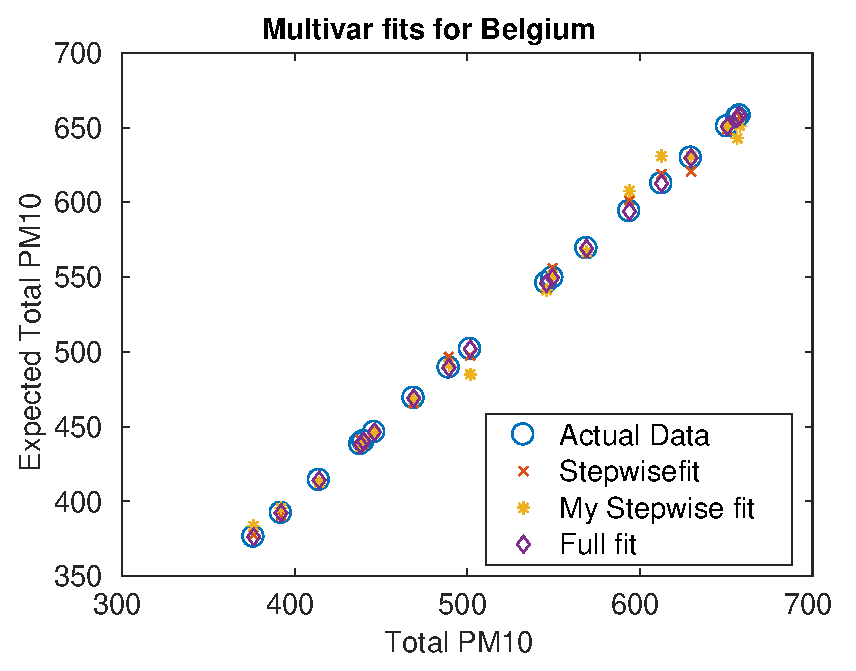
\includegraphics[width=1\columnwidth]{Ex8/Belgium_MultivarFits.eps}	
\caption{Πραγματικές και εκτιμούμενες τιμές για την Belgium.}
\label{fig:z82}
\end{figure}

\begin{Verbatim}[fontsize=\small]
Multivariable fitting for Activities in Country
 	 	 Belgium

                                           Stepwisefit    MyStepwise      Full   
                                           ___________    __________    _________

    AdjR2                                  0.9973         0.99169               1
    Intercept                                23.9          72.856        0.043911
    Agriculture                                 0               0         0.99905
    EnergyIndustries                       1.2977          1.3598         0.99873
    EnergyIndustriesPowerProduction1A1a         0               0       0.0006567
    FugitiveEmissions                           0               0          1.0159
    IndustryEnergy                              0               0          1.0068
    IndustryProcesses                      1.9938               0         0.99274
    OtherEnergy                                 0               0          1.0051
    OtherTransport                              0               0         0.98095
    RoadTransport                          1.7411          2.0741          1.0033
    Waste                                       0               0         0.97523
\end{[fontsize=\small]erbatim}



\begin{figure}[H]

	\centering
	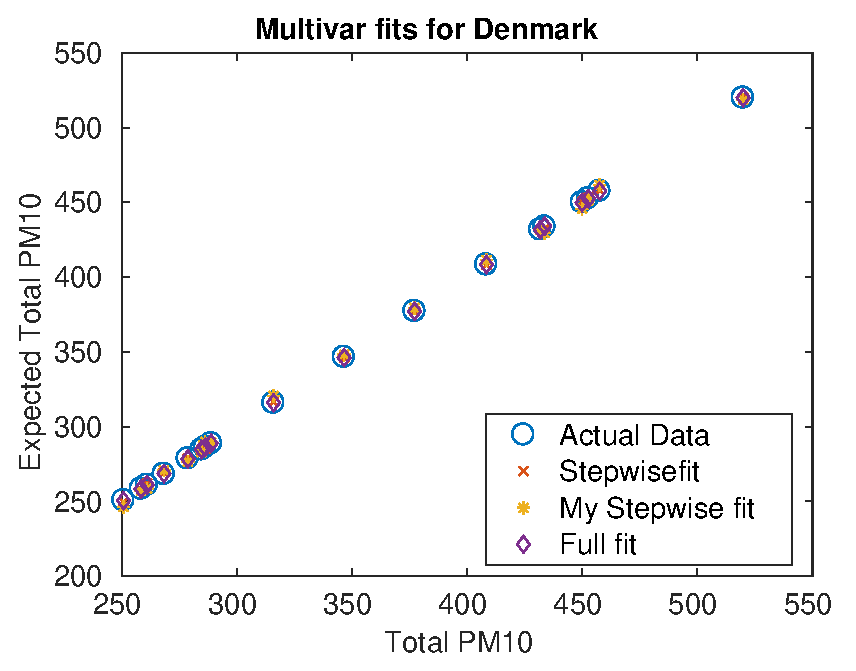
\includegraphics[width=1\columnwidth]{Ex8/Denmark_MultivarFits.eps}	
\caption{Πραγματικές και εκτιμούμενες τιμές για την Denmark.}
\label{fig:z83} 
\end{figure}


\begin{Verbatim}[fontsize=\small]
Multivariable fitting for Activities in Country
 	 	 Denmark

                                           Stepwisefit    MyStepwise     Full  
                                           ___________    __________    _______

    AdjR2                                  0.99992        0.99872       0.99999
    Intercept                               99.167         77.733        25.889
    Agriculture                            0.97628              0       0.97618
    EnergyIndustries                             0              0       0.60969
    EnergyIndustriesPowerProduction1A1a      1.015         1.0301       0.39125
    FugitiveEmissions                            0              0       0.15607
    IndustryEnergy                               0              0       0.74619
    IndustryProcesses                      -6.6942              0       0.12353
    OtherEnergy                                  0              0       0.90714
    OtherTransport                               0              0       0.72493
    RoadTransport                           1.5213         2.1126        1.1612
    Waste                                  -1943.7              0       -579.13
\end{Verbatim}



\begin{figure}[H]

	\centering
	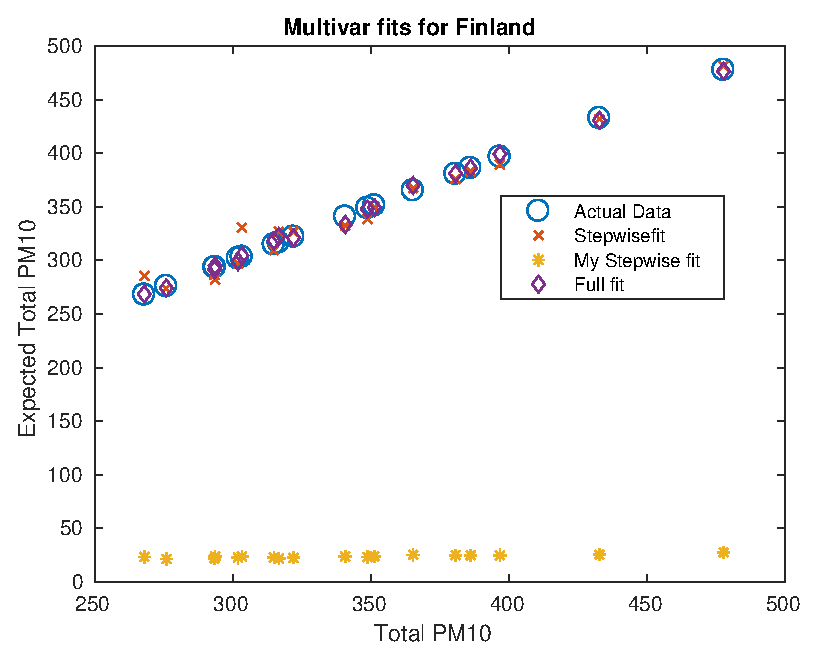
\includegraphics[width=1\columnwidth]{Ex8/Finland_MultivarFits.eps}	
\caption{Πραγματικές και εκτιμούμενες τιμές για την Finland.}
\label{fig:z84} 
\end{figure}



\begin{Verbatim}[fontsize=\small]
Multivariable fitting for Activities in Country
 	 	 Finland

                                           Stepwisefit    MyStepwise      Full  
                                           ___________    ___________    _______

    AdjR2                                  0.95853                  1    0.99306
    Intercept                              -94.508          1.146e-12     61.973
    Agriculture                             12.453                  1       12.9
    EnergyIndustries                             0        -7.0018e-14     -36.27
    EnergyIndustriesPowerProduction1A1a     1.0375         3.7329e-14     37.026
    FugitiveEmissions                      -8.9045        -3.6758e-14    -12.193
    IndustryEnergy                               0         1.4721e-14    -2.7344
    IndustryProcesses                            0        -5.0031e-15     1.8925
    OtherEnergy                             3.1798         -6.584e-15     1.8574
    OtherTransport                               0                  0    -1.8328
    RoadTransport                                0         5.6423e-15     3.6639
    Waste                                        0         7.2905e-13    -139.65
\end{Verbatim}


\begin{figure}[H]
 
	\centering
	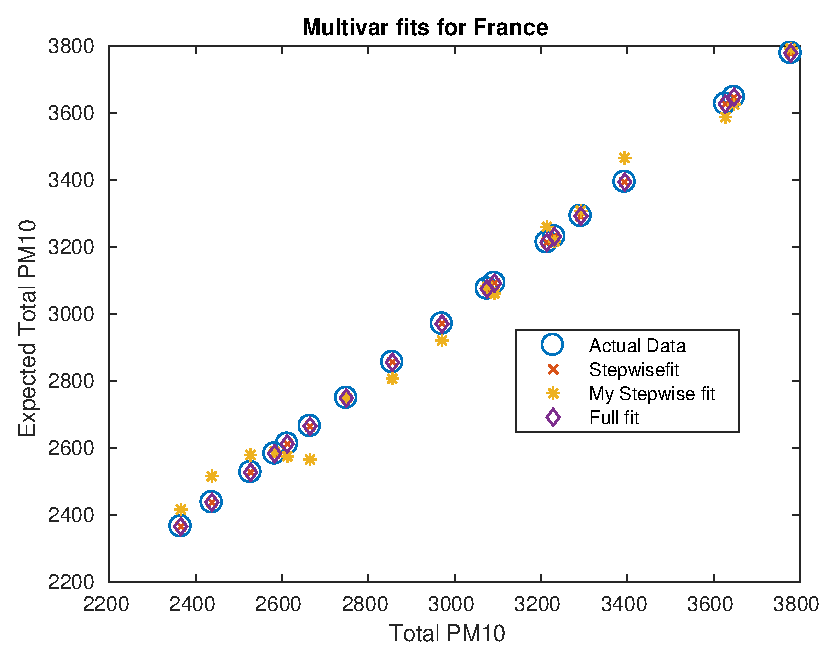
\includegraphics[width=1\columnwidth]{Ex8/France_MultivarFits.eps}	
\caption{Πραγματικές και εκτιμούμενες τιμές για την France.}
\label{fig:z85}
\end{figure}



\begin{Verbatim}[fontsize=\small]
Multivariable fitting for Activities in Country
 	 	 France

                                           Stepwisefit    MyStepwise      Full   
                                           ___________    __________    _________

    AdjR2                                        1        0.98652               1
    Intercept                               1.6751         910.65          1.2303
    Agriculture                             1.0024              0          1.0034
    EnergyIndustries                        1.0005              0         0.99795
    EnergyIndustriesPowerProduction1A1a          0              0       0.0025802
    FugitiveEmissions                      0.99873              0         0.99905
    IndustryEnergy                          0.9998         3.2067          1.0002
    IndustryProcesses                       1.0048              0          1.0015
    OtherEnergy                            0.99996         3.0522         0.99977
    OtherTransport                         0.99356              0          0.9952
    RoadTransport                           1.0003              0          1.0004
    Waste                                  0.98949              0         0.98796
\end{Verbatim}


\begin{figure}[H]
 
	\centering
	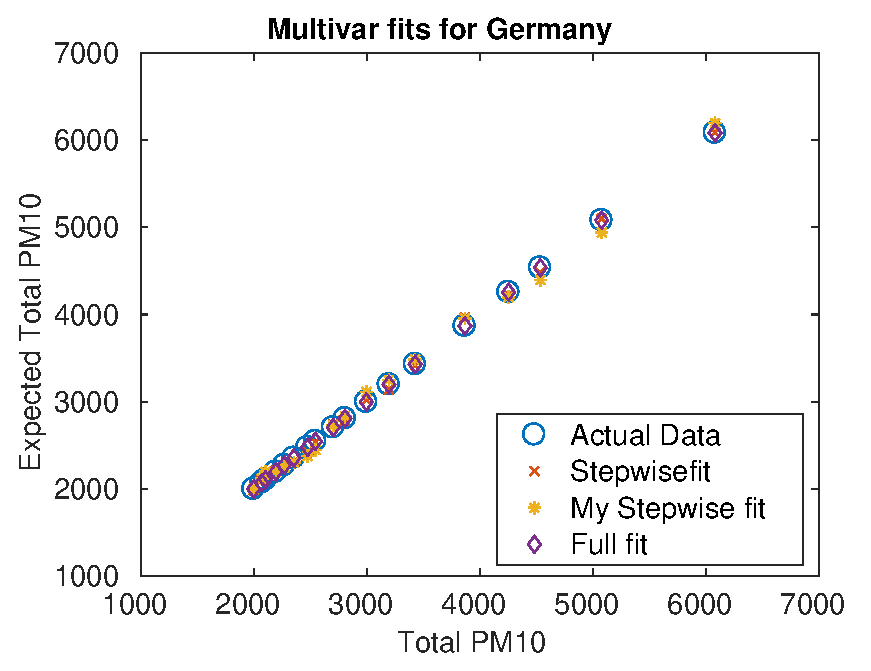
\includegraphics[width=1\columnwidth]{Ex8/Germany_MultivarFits.eps}	
\caption{Πραγματικές και εκτιμούμενες τιμές για την Germany.}
\label{fig:z86}
\end{figure}



\begin{Verbatim}[fontsize=\small]
Multivariable fitting for Activities in Country
 	 	 Germany

                                           Stepwisefit    MyStepwise       Full   
                                           ___________    __________    __________

    AdjR2                                  0.99805        0.99425                1
    Intercept                               307.72         795.46           11.214
    Agriculture                                  0              0           1.0008
    EnergyIndustries                             0              0           1.0005
    EnergyIndustriesPowerProduction1A1a          0              0       -0.0010719
    FugitiveEmissions                      -31.288              0           1.0111
    IndustryEnergy                          3.8509         3.2964          0.99969
    IndustryProcesses                       2.5244              0          0.99878
    OtherEnergy                                  0              0                1
    OtherTransport                          13.477         11.207           1.0002
    RoadTransport                                0              0           1.0001
    Waste                                        0              0           2.9314
\end{Verbatim}



\begin{figure}[H]

	\centering
	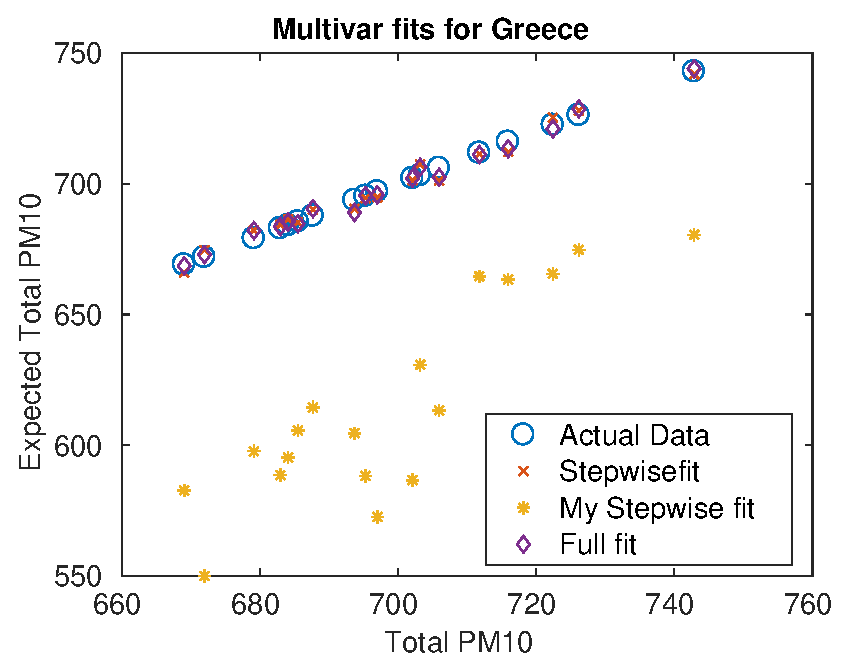
\includegraphics[width=1\columnwidth]{Ex8/Greece_MultivarFits.eps}	
\caption{Πραγματικές και εκτιμούμενες τιμές για την Greece.}
\label{fig:z87} 
\end{figure}



\begin{Verbatim}[fontsize=\small]
Multivariable fitting for Activities in Country
 	 	 Greece

                                           Stepwisefit    MyStepwise     Full  
                                           ___________    __________    _______

    AdjR2                                  0.97082        0.89938          0.97
    Intercept                               48.079         192.78       -67.767
    Agriculture                                  0              0        1.6209
    EnergyIndustries                             0              0       0.81668
    EnergyIndustriesPowerProduction1A1a     1.1346         1.0904       0.28362
    FugitiveEmissions                            0              0         1.733
    IndustryEnergy                         0.89349              0       0.92504
    IndustryProcesses                       4.5881         1.1541        3.9211
    OtherEnergy                            0.94408              0       0.78521
    OtherTransport                         0.90138        0.98916        0.8848
    RoadTransport                          0.68783              0       0.97042
    Waste                                        0              0             0
\end{Verbatim}



\begin{figure}[H]

	\centering
	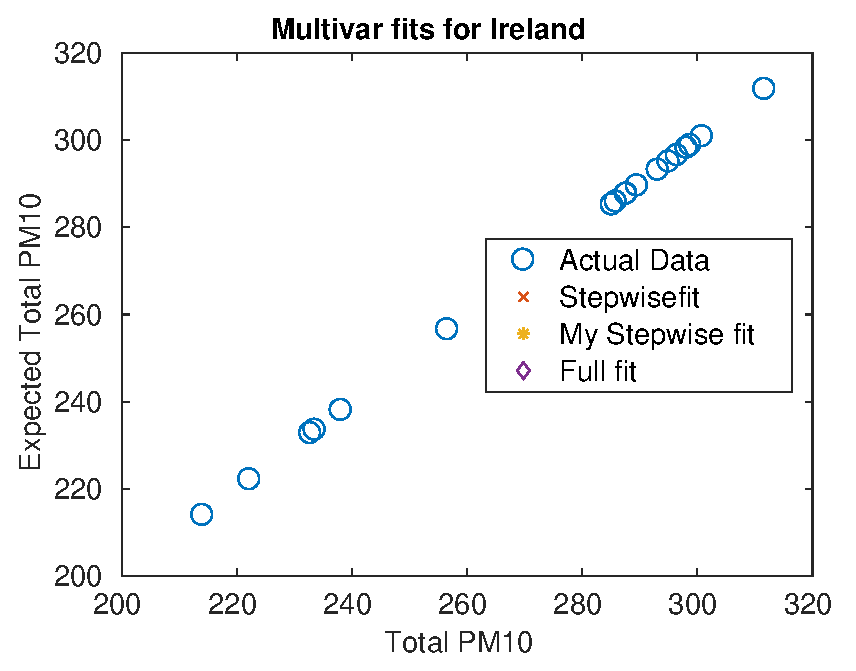
\includegraphics[width=1\columnwidth]{Ex8/Ireland_MultivarFits.eps}	
\caption{Πραγματικές και εκτιμούμενες τιμές για την Ireland.}
\label{fig:z88} 
\end{figure}



\begin{Verbatim}[fontsize=\small]
Multivariable fitting for Activities in Country
 	 	 Ireland

                                           Stepwisefit    MyStepwise    Full
                                           ___________    __________    ____

    AdjR2                                  NaN            NaN           NaN 
    Intercept                                0              0             0 
    Agriculture                            NaN              0             0 
    EnergyIndustries                       NaN              0             0 
    EnergyIndustriesPowerProduction1A1a    NaN              0             0 
    FugitiveEmissions                      NaN              0             0 
    IndustryEnergy                         NaN              0             0 
    IndustryProcesses                      NaN              0             0 
    OtherEnergy                            NaN              0             0 
    OtherTransport                         NaN              0             0 
    RoadTransport                          NaN              0             0 
    Waste                                  NaN              0             0
\end{Verbatim}



\begin{figure}[H]

	\centering
	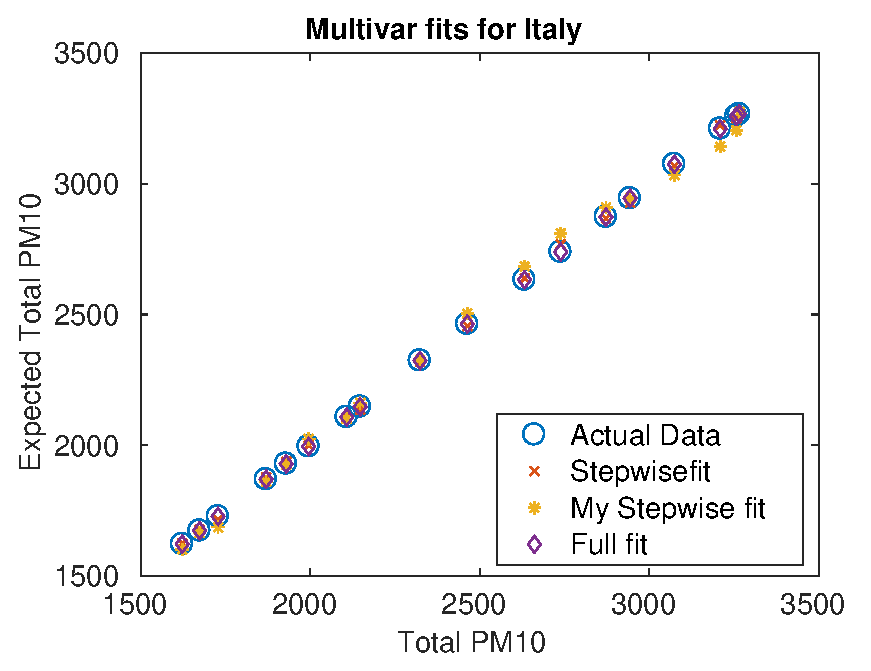
\includegraphics[width=1\columnwidth]{Ex8/Italy_MultivarFits.eps}	
\caption{Πραγματικές και εκτιμούμενες τιμές για την Italy.}
\label{fig:z89} 
\end{figure}



\begin{Verbatim}[fontsize=\small]
Multivariable fitting for Activities in Country
 	 	 Italy

                                           Stepwisefit    MyStepwise      Full   
                                           ___________    __________    _________

    AdjR2                                  0.99955        0.99535               1
    Intercept                               236.84         795.77         -8.4128
    Agriculture                                  0              0          1.0478
    EnergyIndustries                        1.1083          1.601           1.015
    EnergyIndustriesPowerProduction1A1a          0              0       -0.020811
    FugitiveEmissions                            0              0         0.96018
    IndustryEnergy                         0.73009              0         0.99561
    IndustryProcesses                            0              0         0.99623
    OtherEnergy                             2.4875              0          1.0249
    OtherTransport                               0              0          1.0093
    RoadTransport                           1.3897        0.95283         0.99966
    Waste                                        0              0         0.94412
\end{Verbatim}



\begin{figure}[H]

	\centering
	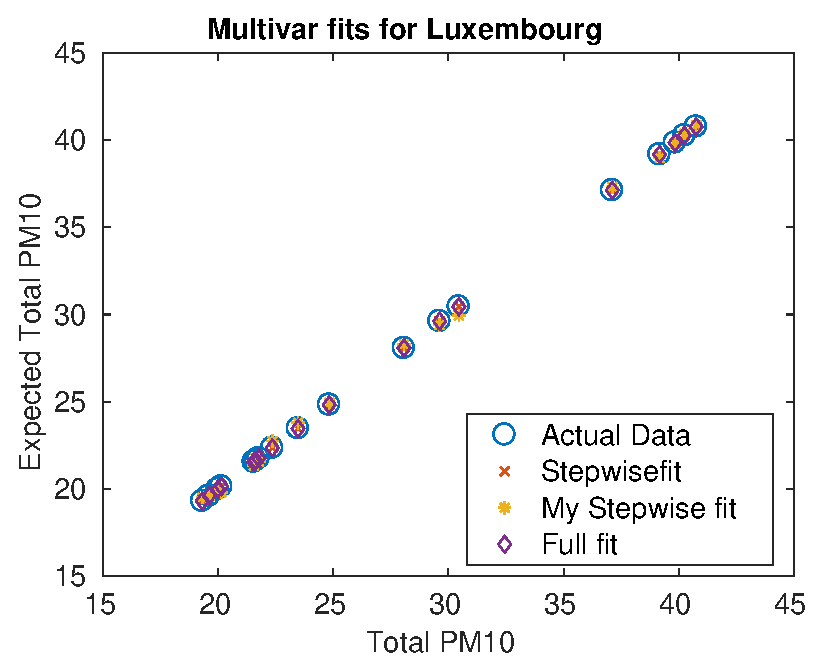
\includegraphics[width=1\columnwidth]{Ex8/Luxembourg_MultivarFits.eps}	
\caption{Πραγματικές και εκτιμούμενες τιμές για την Luxembourg.}
\label{fig:z810} 
\end{figure}



\begin{Verbatim}[fontsize=\small]
Multivariable fitting for Activities in Country
 	 	 Luxembourg

T =

  12×3 table

                                           Stepwisefit    MyStepwise     Full  
                                           ___________    __________    _______

    AdjR2                                        1        0.99902             1
    Intercept                              0.44334         8.2746       0.43625
    Agriculture                             1.0431              0        1.0431
    EnergyIndustries                       0.98625              0       0.98621
    EnergyIndustriesPowerProduction1A1a          0              0             0
    FugitiveEmissions                      -9.0633              0       -9.0182
    IndustryEnergy                          1.0004         1.1554        1.0004
    IndustryProcesses                        1.001              0        1.0011
    OtherEnergy                            0.99722              0       0.99727
    OtherTransport                          0.9718              0       0.97168
    RoadTransport                           1.0058        0.72766        1.0058
    Waste                                        0              0       0.57505
\end{Verbatim}



\begin{figure}[H]

	\centering
	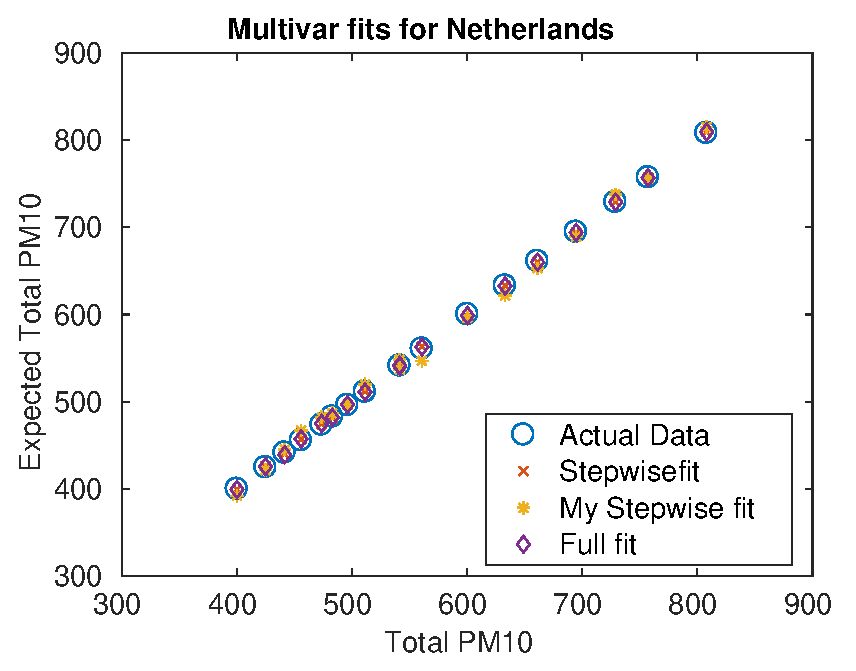
\includegraphics[width=1\columnwidth]{Ex8/Netherlands_MultivarFits.eps}	
\caption{Πραγματικές και εκτιμούμενες τιμές για την Netherlands.}
\label{fig:z811} 
\end{figure}



\begin{Verbatim}[fontsize=\small]
Multivariable fitting for Activities in Country
 	 	 Netherlands

                                           Stepwisefit    MyStepwise      Full  
                                           ___________    __________    ________

    AdjR2                                  0.99979        0.99557        0.99979
    Intercept                              -27.708         2.0338         -24.21
    Agriculture                            0.72279              0        0.82979
    EnergyIndustries                       0.96859              0        0.97796
    EnergyIndustriesPowerProduction1A1a          0              0       -0.05186
    FugitiveEmissions                       1.4303              0         1.3791
    IndustryEnergy                          1.0973         1.2597         1.0776
    IndustryProcesses                      0.87159              0        0.95956
    OtherEnergy                                  0              0        0.63861
    OtherTransport                          1.3765              0          1.153
    RoadTransport                           1.2703          2.944         1.1673
    Waste                                        0              0         1.3544
\end{Verbatim}



\begin{figure}[H]

	\centering
	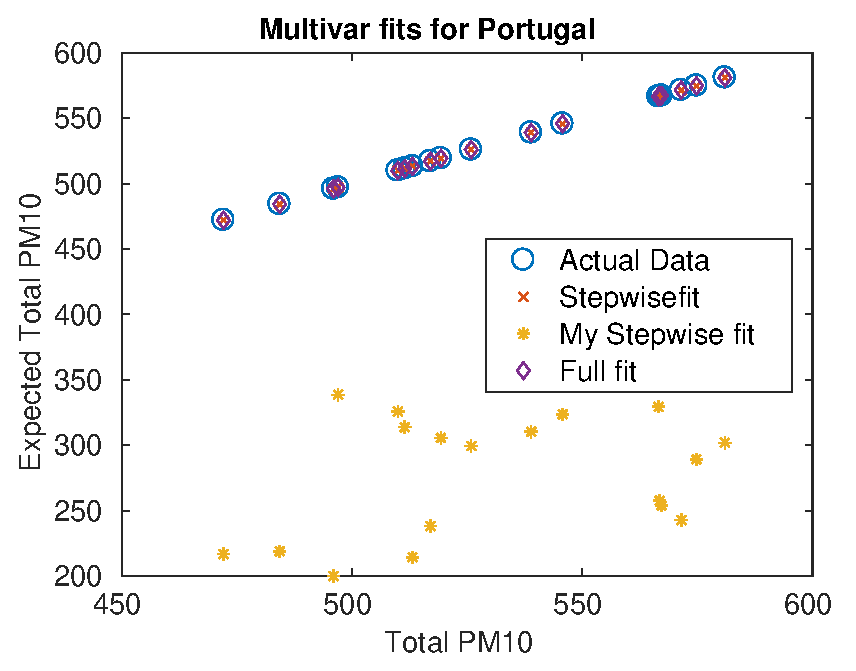
\includegraphics[width=1\columnwidth]{Ex8/Portugal_MultivarFits.eps}	
\caption{Πραγματικές και εκτιμούμενες τιμές για την Portugal.}
\label{fig:z812} 
\end{figure}



\begin{Verbatim}[fontsize=\small]
Multivariable fitting for Activities in Country
 	 	 Portugal

                                           Stepwisefit    MyStepwise     Full  
                                           ___________    __________    _______

    AdjR2                                  0.99999        0.86944             1
    Intercept                               3.4454         117.28        2.8042
    Agriculture                            0.89938         9.5993       0.93988
    EnergyIndustries                       0.99466        0.94915       0.98177
    EnergyIndustriesPowerProduction1A1a          0              0       0.01454
    FugitiveEmissions                      0.91417              0       0.97735
    IndustryEnergy                          1.0218              0        1.0156
    IndustryProcesses                      0.99696              0       0.99753
    OtherEnergy                              1.027              0        1.0136
    OtherTransport                          0.9982              0       0.98878
    RoadTransport                           1.0002        -3.9099        1.0026
    Waste                                  0.95391              0       0.97481
\end{Verbatim}



\begin{figure}[H]

	\centering
	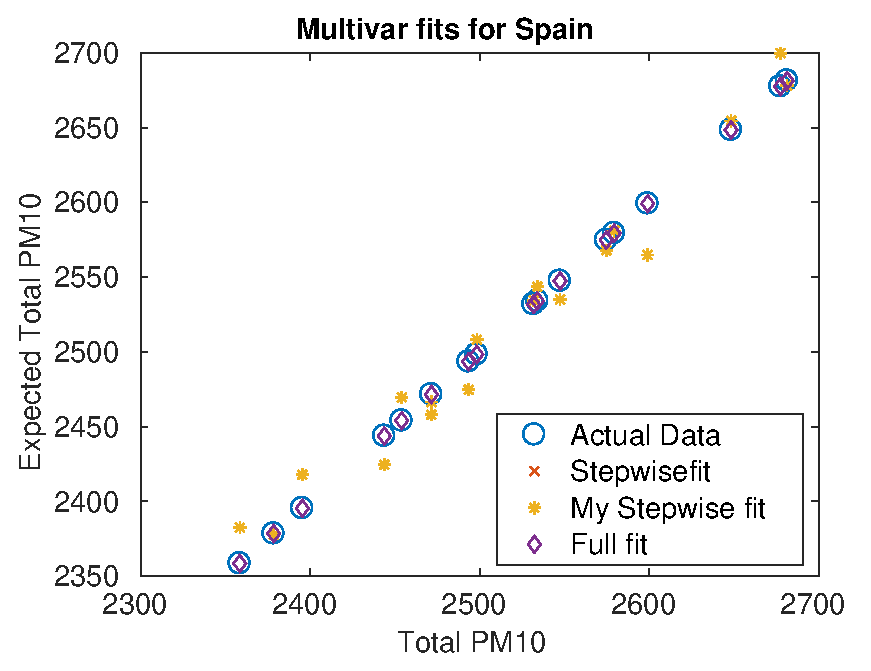
\includegraphics[width=1\columnwidth]{Ex8/Spain_MultivarFits.eps}	
\caption{Πραγματικές και εκτιμούμενες τιμές για την Spain.}
\label{fig:z813} 
\end{figure}



\begin{Verbatim}[fontsize=\small]
Multivariable fitting for Activities in Country
 	 	 Spain

                                           Stepwisefit    MyStepwise       Full   
                                           ___________    __________    __________

    AdjR2                                  0.96882        0.96882                1
    Intercept                               1275.1         1275.1       1.7906e-05
    Agriculture                                  0              0                1
    EnergyIndustries                       0.91608        0.91608                1
    EnergyIndustriesPowerProduction1A1a          0              0       4.7977e-08
    FugitiveEmissions                            0              0                1
    IndustryEnergy                               0              0                1
    IndustryProcesses                            0              0                1
    OtherEnergy                             5.5264         5.5264                1
    OtherTransport                               0              0                1
    RoadTransport                                0              0                1
    Waste                                        0              0                1
\end{Verbatim}



\begin{figure}[H]

	\centering
	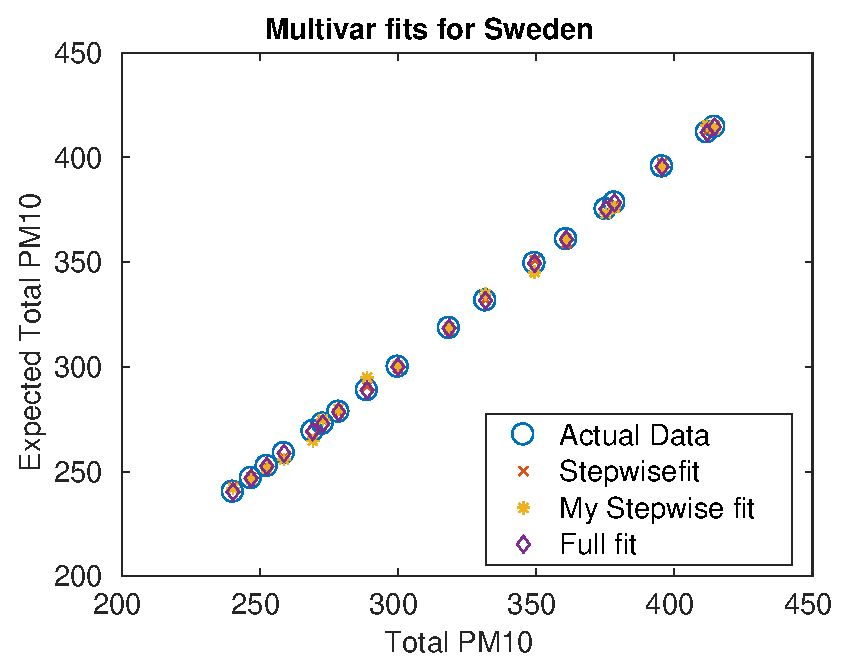
\includegraphics[width=1\columnwidth]{Ex8/Sweden_MultivarFits.eps}	
\caption{Πραγματικές και εκτιμούμενες τιμές για την Sweden.}
\label{fig:z814} 
\end{figure}



\begin{Verbatim}[fontsize=\small]

Multivariable fitting for Activities in Country
 	 	 Sweden

                                           Stepwisefit    MyStepwise      Full   
                                           ___________    __________    _________

    AdjR2                                   0.9992        0.9976                1
    Intercept                               56.276        59.476           1.1726
    Agriculture                                  0             0           1.0118
    EnergyIndustries                             0             0           1.0408
    EnergyIndustriesPowerProduction1A1a    0.81219             0        -0.036913
    FugitiveEmissions                            0             0          0.96369
    IndustryEnergy                               0             0          0.99073
    IndustryProcesses                       1.8515        2.2998          0.98606
    OtherEnergy                                  0             0           1.0346
    OtherTransport                               0             0          0.99516
    RoadTransport                           1.4246        1.4017          0.99781
    Waste                                        0             0          0.59146
\end{Verbatim}



\begin{figure}[H]
 
	\centering
	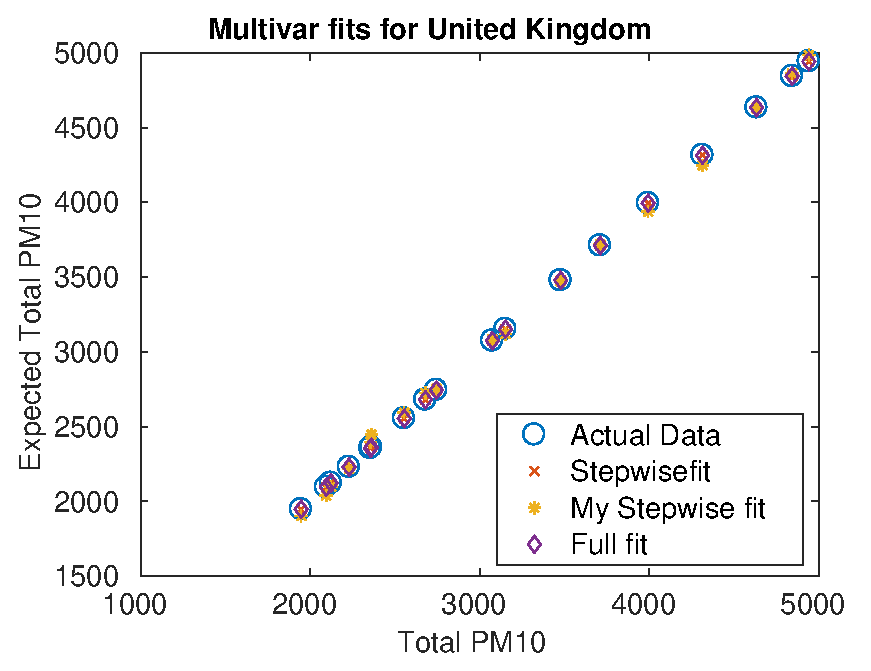
\includegraphics[width=1\columnwidth]{Ex8/United-Kingdom_MultivarFits.eps}	
\caption{Πραγματικές και εκτιμούμενες τιμές για την United Kingdom.}
\label{fig:z815}
\end{figure}



\begin{Verbatim}[fontsize=\small]
Multivariable fitting for Activities in Country
 	 	 United Kingdom

                                           Stepwisefit    MyStepwise      Full  
                                           ___________    __________    ________

    AdjR2                                        1        0.99806              1
    Intercept                               4.7657         530.96         11.531
    Agriculture                             1.0324              0         1.0613
    EnergyIndustries                        1.0006         1.1866        0.92625
    EnergyIndustriesPowerProduction1A1a          0              0       0.074051
    FugitiveEmissions                      0.97923              0         1.0038
    IndustryEnergy                          1.0092              0          1.008
    IndustryProcesses                       1.0837              0         1.1626
    OtherEnergy                            0.99949              0         1.0115
    OtherTransport                         0.98561              0        0.96598
    RoadTransport                          0.98992         1.5858        0.98476
    Waste                                  0.94384              0        0.87251
\end{Verbatim}














\subsection{Ζήτημα 9}
\label{subsec:z9}

Για την επίλυση αυτού του ζητήματος κάνουμε χρήση του \hyperref[mat:9]{κώδικα \ref*{mat:9}}. Εκτελώντας τον παραπάνω κώδικα για κάθε δραστηριότητα για την Greece, παίρνουμε τα παρακάτω αποτελέσματα.






\begin{figure}[H]

	\centering
	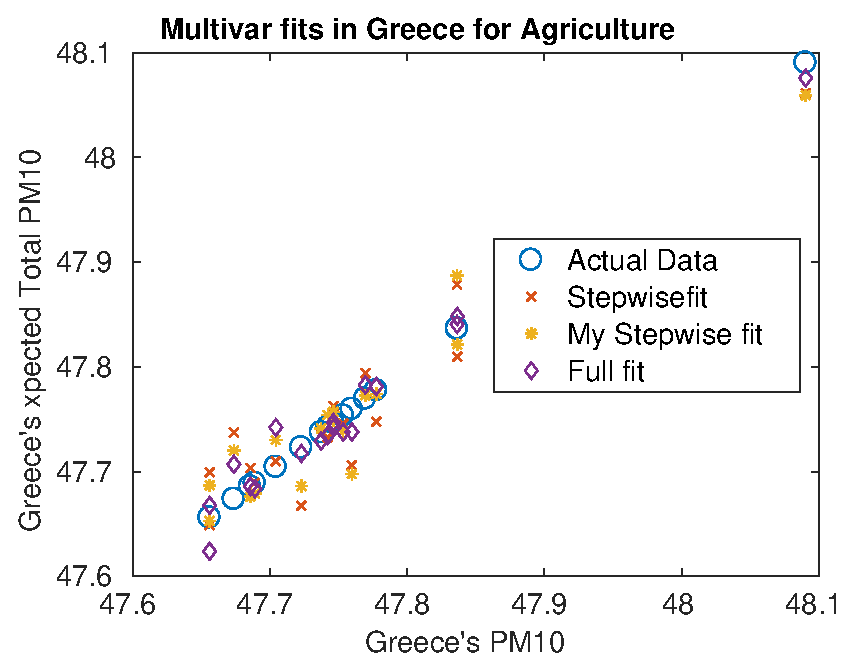
\includegraphics[width=1\columnwidth]{Ex9/Agriculture_Greece_MultivarFits.eps}	
\caption{Πραγματικές και εκτιμούμενες τιμές για την Agriculture.}
\label{fig:z91} 
\end{figure}



\begin{Verbatim}[fontsize=\small]
Multivariable fitting in Greece for activity
 	 	 Agriculture

                      Stepwisefit    MyStepwise       Full    
                      ___________    __________    ___________

    AdjR2                0.86178        0.88512        0.82286
    Intercept             45.596         45.702         47.088
    Austria                    0              0       0.096335
    Belgium            -0.015028      -0.015874      -0.017953
    Denmark                    0        0.00443      -0.015499
    Finland                    0              0       0.027114
    France                     0              0     -0.0072636
    Germany           -0.0039902     -0.0041459    -4.3904e-05
    Ireland                    0              0       0.031979
    Italy                      0              0      0.0064466
    Luxembourg           0.81344        0.85913       -0.79274
    Netherlands                0              0      0.0072244
    Portugal                   0              0        0.07024
    Spain                      0              0     -0.0046717
    Sweden                     0              0      -0.048242
    United Kingdom       0.01214       0.010109    -0.00068957
\end{Verbatim}




\begin{figure}[H]

	\centering
	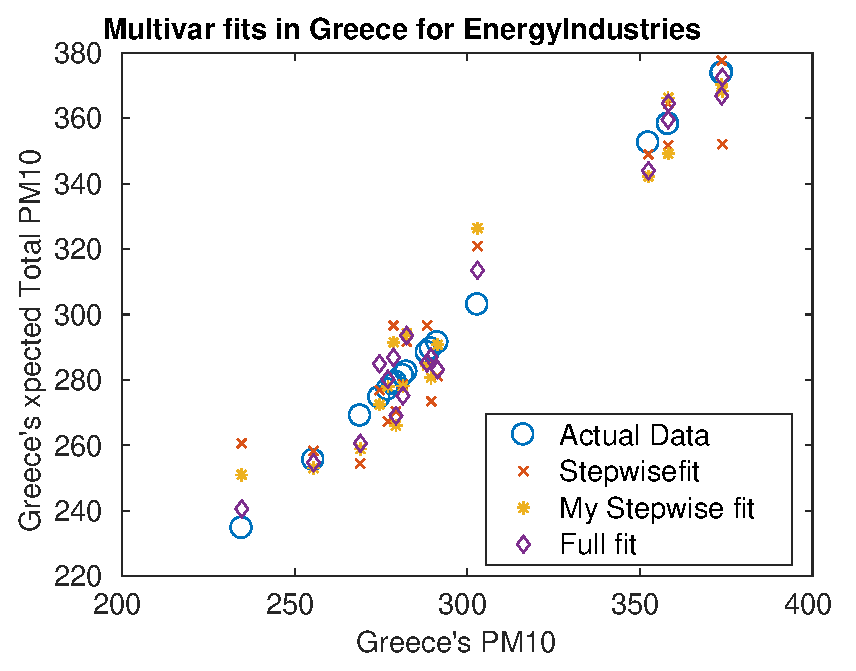
\includegraphics[width=1\columnwidth]{Ex9/EnergyIndustries_Greece_MultivarFits.eps}	
\caption{Πραγματικές και εκτιμούμενες τιμές για την EnergyIndustries.}
\label{fig:z92} 
\end{figure}



\begin{Verbatim}[fontsize=\small]

Multivariable fitting in Greece for activity
 	 	 EnergyIndustries
 	 	 
                      Stepwisefit    MyStepwise      Full  
                      ___________    __________    ________

    AdjR2             0.90198          0.92286      0.83018
    Intercept          474.51           467.32       296.64
    Austria                 0                0        1.949
    Belgium                 0                0       1.9156
    Denmark                 0                0     0.052545
    Finland                 0         -0.61138      0.69142
    France                  0                0      0.25209
    Germany                 0                0      0.11984
    Ireland           -2.0901          -0.9729      -3.9346
    Italy                   0                0     -0.20664
    Luxembourg              0           47.594      -49.602
    Netherlands             0                0      0.83065
    Portugal                0                0       1.3159
    Spain                   0        -0.077521      0.02111
    Sweden                  0                0      0.88024
    United Kingdom          0                0       -0.245
\end{Verbatim}


\begin{figure}[H]

	\centering
	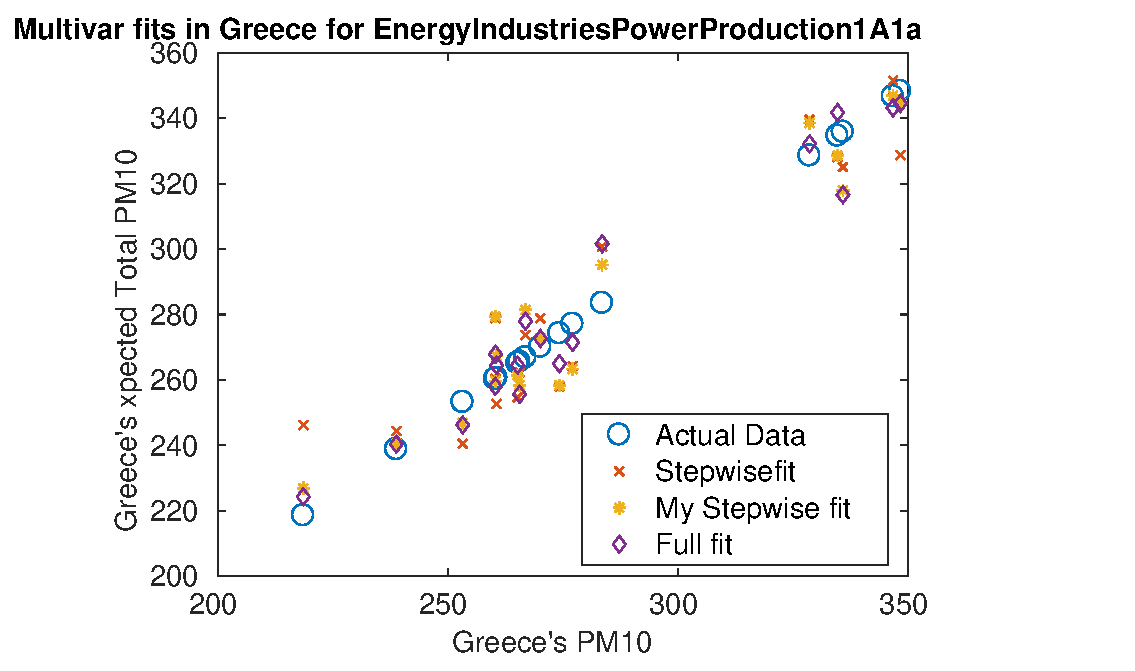
\includegraphics[width=1\columnwidth]{Ex9/EnergyIndustriesPowerProduction1A1a_Greece_MultivarFits.eps}	
\caption{Πραγματικές και εκτιμούμενες τιμές για την EnergyIndustriesPowerProduction1A1a.}
\label{fig:z93} 
\end{figure}



\begin{Verbatim}[fontsize=\small]
Multivariable fitting in Greece for activity
 	 	 EnergyIndustriesPowerProduction1A1a

                      Stepwisefit    MyStepwise      Full  
                      ___________    __________    ________

    AdjR2             0.87445         0.89708       0.71327
    Intercept          434.55          387.12        259.41
    Austria                 0               0        -1.088
    Belgium                 0         0.73171        3.2609
    Denmark                 0               0        0.6597
    Finland                 0        -0.39525        1.8287
    France                  0               0       0.16972
    Germany                 0               0       0.20092
    Ireland           -1.8594         -1.3344       -4.7954
    Italy                   0        -0.14575      -0.37673
    Luxembourg              0               0        -91.87
    Netherlands             0               0       0.79198
    Portugal                0               0        2.0357
    Spain                   0               0       0.13377
    Sweden                  0          1.8285       -1.9564
    United Kingdom          0               0      -0.28303
\end{Verbatim}


\begin{figure}[H]
 
	\centering
	\includegraphics[width=1\columnwidth]{Ex9/FugitiveEmissions_Greece_MultivarFits.eps}	
\caption{Πραγματικές και εκτιμούμενες τιμές για την FugitiveEmissions.}
\label{fig:z94}
\end{figure}



\begin{Verbatim}[fontsize=\small]
Multivariable fitting in Greece for activity
 	 	 FugitiveEmissions

                      Stepwisefit    MyStepwise      Full   
                      ___________    __________    _________

    AdjR2                  0          0.77567        0.53648
    Intercept         6.6644            9.592         10.814
    Austria                0          0.99219         1.6424
    Belgium                0                0      -0.092541
    Denmark                0                0        0.76422
    Finland                0         0.076773       0.085452
    France                 0                0       0.022749
    Germany                0                0       0.016665
    Ireland                0                0        -32.693
    Italy                  0                0       0.032679
    Luxembourg             0                0        -6.5289
    Netherlands            0                0       -0.01197
    Portugal               0         -0.58438       -0.62403
    Spain                  0         0.041141      0.0066155
    Sweden                 0                0       -0.36538
    United Kingdom         0         -0.18922        -0.3308
\end{Verbatim}



\begin{figure}[H]

	\centering
	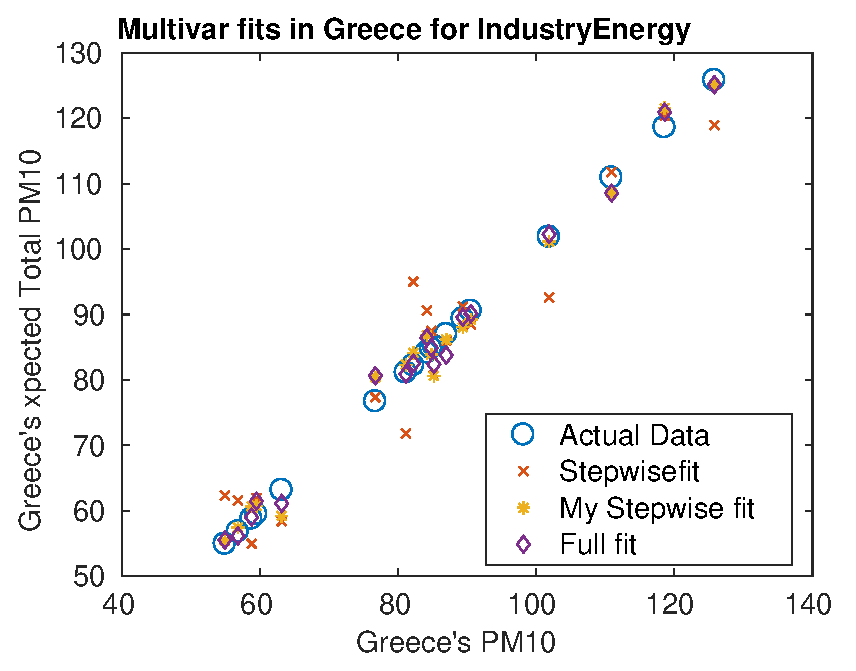
\includegraphics[width=1\columnwidth]{Ex9/IndustryEnergy_Greece_MultivarFits.eps}	
\caption{Πραγματικές και εκτιμούμενες τιμές για την IndustryEnergy.}
\label{fig:z95} 
\end{figure}



\begin{Verbatim}[fontsize=\small]
Multivariable fitting in Greece for activity
 	 	 IndustryEnergy

                      Stepwisefit    MyStepwise      Full   
                      ___________    __________    _________

    AdjR2             0.90343          0.97125       0.95425
    Intercept         -119.16          -35.916        119.11
    Austria                 0                0        2.1411
    Belgium                 0           2.0229        1.8359
    Denmark                 0                0       -5.0327
    Finland           0.37344        -0.015284       -0.1505
    France            0.35764         0.017361       0.12145
    Germany                 0          0.03927       0.12252
    Ireland                 0         -0.19345        -1.042
    Italy                   0                0     -0.093878
    Luxembourg              0           2.9127       -3.5578
    Netherlands             0                0       -1.2819
    Portugal          0.63502          0.73275       0.54247
    Spain                   0         -0.16366      -0.52836
    Sweden                  0           1.4636        1.8461
    United Kingdom          0         -0.39097       0.10122
\end{Verbatim}


\begin{figure}[H]

	\centering
	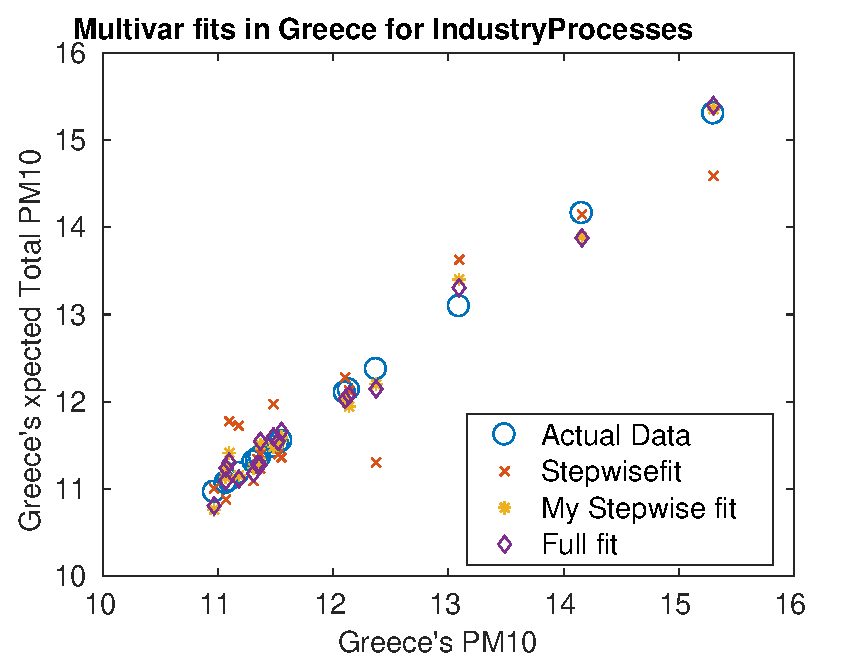
\includegraphics[width=1\columnwidth]{Ex9/IndustryProcesses_Greece_MultivarFits.eps}	
\caption{Πραγματικές και εκτιμούμενες τιμές για την IndustryProcesses.}
\label{fig:z96} 
\end{figure}



\begin{Verbatim}[fontsize=\small]
Multivariable fitting in Greece for activity
 	 	 IndustryProcesses

                      Stepwisefit    MyStepwise       Full   
                      ___________    __________    __________

    AdjR2              0.8488          0.94484         0.9072
    Intercept          3.5538           5.9051         4.7513
    Austria           0.33126          0.29805        0.45469
    Belgium                 0          0.13114        0.14683
    Denmark                 0                0        0.40205
    Finland           0.14777        -0.046504     -0.0028813
    France                  0         -0.14279       -0.15543
    Germany                 0         0.022111       0.021385
    Ireland                 0                0       -0.65945
    Italy                   0        -0.026603      -0.031864
    Luxembourg              0           3.6695         3.6702
    Netherlands             0        -0.053754       -0.03875
    Portugal                0         0.019561       0.024573
    Spain                   0          0.34451        0.30929
    Sweden                  0                0     -0.0072315
    United Kingdom          0        -0.092307      -0.096864
\end{Verbatim}


\begin{figure}[H]
 
	\centering
	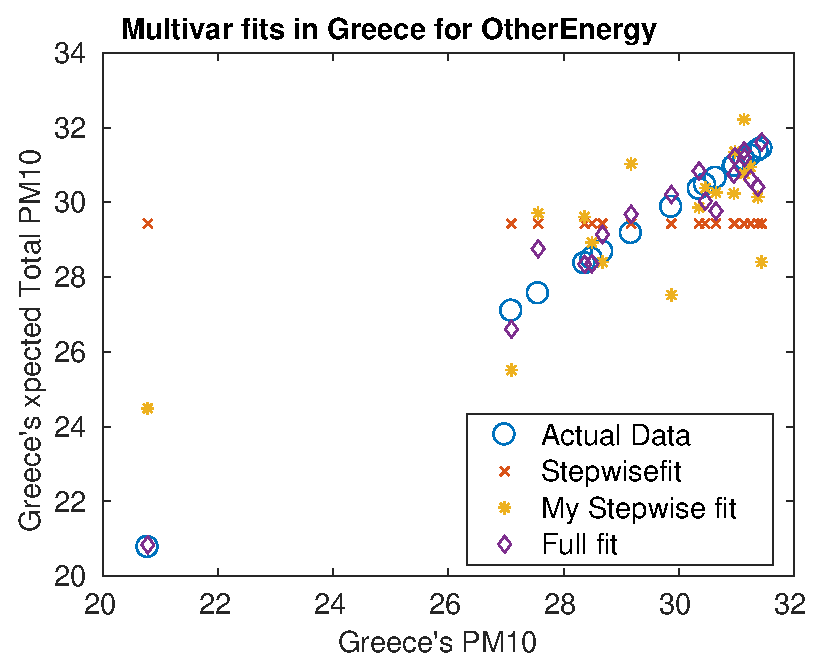
\includegraphics[width=1\columnwidth]{Ex9/OtherEnergy_Greece_MultivarFits.eps}	
\caption{Πραγματικές και εκτιμούμενες τιμές για την OtherEnergy.}
\label{fig:z97}
\end{figure}



\begin{Verbatim}[fontsize=\small]
Multivariable fitting in Greece for activity
 	 	 OtherEnergy

                      Stepwisefit    MyStepwise      Full   
                      ___________    __________    _________

    AdjR2                  0           0.43077       0.74738
    Intercept         29.431            63.618        56.321
    Austria                0          -0.73635       -1.4445
    Belgium                0           0.95897         1.903
    Denmark                0          -0.58404       -1.8441
    Finland                0                 0       0.48462
    France                 0                 0      -0.19306
    Germany                0         0.0010798     -0.076534
    Ireland                0                 0        3.0946
    Italy                  0                 0        0.4919
    Luxembourg             0             -32.7       -39.493
    Netherlands            0                 0       0.53744
    Portugal               0                 0      -0.69296
    Spain                  0                 0      0.047386
    Sweden                 0                 0      -0.64824
    United Kingdom         0                 0      0.050059
\end{Verbatim}



\begin{figure}[H]
 
	\centering
	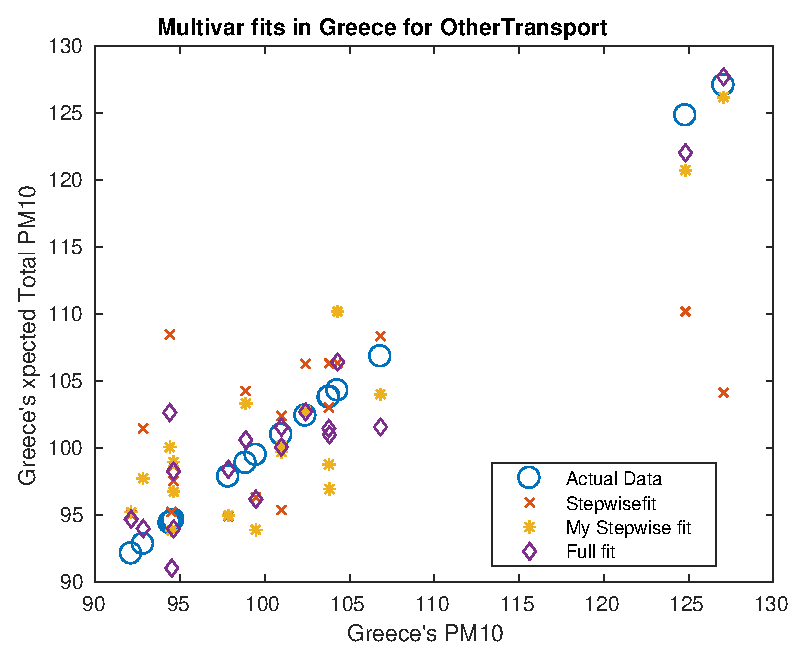
\includegraphics[width=1\columnwidth]{Ex9/OtherTransport_Greece_MultivarFits.eps}	
\caption{Πραγματικές και εκτιμούμενες τιμές για την OtherTransport.}
\label{fig:z98}
\end{figure}



\begin{Verbatim}[fontsize=\small]
Multivariable fitting in Greece for activity
 	 	 OtherTransport

                      Stepwisefit    MyStepwise      Full   
                      ___________    __________    _________

    AdjR2              0.244          0.70262        0.40267
    Intercept          85.82           72.405          591.2
    Austria                0                0        -6.0897
    Belgium                0           1.2661          2.106
    Denmark                0                0        -4.3533
    Finland                0          0.91441         1.3149
    France                 0          0.83505        0.91368
    Germany                0                0       0.071008
    Ireland                0                0         6.0115
    Italy                  0                0        -0.4334
    Luxembourg        82.645           37.353          14.79
    Netherlands            0                0        -1.1693
    Portugal               0          -2.6332        -1.0819
    Spain                  0                0       -0.92951
    Sweden                 0          -4.6855        -6.1015
    United Kingdom         0         -0.10652      -0.081946
\end{Verbatim}



\begin{figure}[H]
 
	\centering
	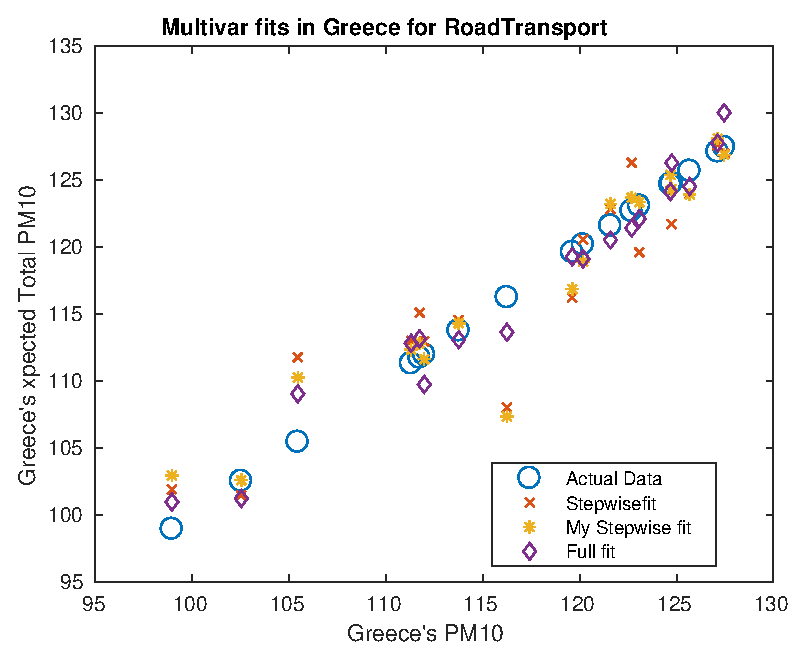
\includegraphics[width=1\columnwidth]{Ex9/RoadTransport_Greece_MultivarFits.eps}	
\caption{Πραγματικές και εκτιμούμενες τιμές για την RoadTransport.}
\label{fig:z99}
\end{figure}



\begin{Verbatim}[fontsize=\small]
Multivariable fitting in Greece for activity
 	 	 RoadTransport

                      Stepwisefit    MyStepwise      Full   
                      ___________    __________    _________

    AdjR2              0.83639        0.85769        0.77331
    Intercept           10.724         38.682          42.24
    Austria                  0              0        0.33988
    Belgium                  0              0        0.63679
    Denmark                  0              0        -1.3146
    Finland                  0              0        0.13043
    France                   0              0       0.089271
    Germany                  0              0      0.0024107
    Ireland                  0              0      -0.025922
    Italy                    0              0       -0.14636
    Luxembourg               0              0       -0.43498
    Netherlands              0       -0.20742       -0.48155
    Portugal          -0.29601         -0.163        -1.0821
    Spain              0.24652         0.1776        0.28207
    Sweden                   0              0       -0.46734
    United Kingdom           0       0.042191        0.21825
\end{Verbatim}



\begin{figure}[H]

	\centering
	\includegraphics[width=1\columnwidth]{Ex9/Waste_Greece_MultivarFits.eps}	
\caption{Πραγματικές και εκτιμούμενες τιμές για την Waste.}
\label{fig:z910} 
\end{figure}



\begin{Verbatim}[fontsize=\small]
Multivariable fitting in Greece for activity
 	 	 Waste

                      Stepwisefit    MyStepwise    Full
                      ___________    __________    ____

    AdjR2             NaN            NaN           NaN 
    Intercept           0              0             0 
    Austria           NaN              0             0 
    Belgium           NaN              0             0 
    Denmark           NaN              0             0 
    Finland           NaN              0             0 
    France            NaN              0             0 
    Germany           NaN              0             0 
    Ireland           NaN              0             0 
    Italy             NaN              0             0 
    Luxembourg        NaN              0             0 
    Netherlands       NaN              0             0 
    Portugal          NaN              0             0 
    Spain             NaN              0             0 
    Sweden            NaN              0             0 
    United Kingdom    NaN              0             0 
\end{Verbatim}








\subsection{Ζήτημα 10}
\label{subsec:z10}


Για την επίλυση αυτού του ζητήματος κάνουμε χρήση του \hyperref[mat:10]{κώδικα \ref*{mat:10}}. Εκτελώντας τον παραπάνω κώδικα για 10 τυχαία ζεύγη δραστηριοτήτων και χωρών και επιλέγοντας σε κάθε ένα πολυώνυμο βαθμού 1 παίρνουμε τα παρακάτω αποτελέσματα.



\begin{figure}[H]

	\centering
	\includegraphics[width=1\columnwidth]{Ex10/Belgium_EnergyIndustries_Trend_and_Corr.eps}	
\caption{Διάγραμμα ιστορίας για την χώρα Belgium και δραστηριότητα EnergyIndustries.}
\label{fig:z101} 
\end{figure}


\begin{figure}[H]
 
	\centering
	\includegraphics[width=1\columnwidth]{Ex10/Belgium_Waste_Trend_and_Corr.eps}	
\caption{Διάγραμμα ιστορίας για την χώρα Belgium και δραστηριότητα Waste.}
\label{fig:z102}
\end{figure}


\begin{figure}[H]

	\centering
	\includegraphics[width=1\columnwidth]{Ex10/France_IndustryEnergy_Trend_and_Corr.eps}	
\caption{Διάγραμμα ιστορίας για την χώρα France και δραστηριότητα IndustryEnergy.}
\label{fig:z103} 
\end{figure}


\begin{figure}[H]

	\centering
	\includegraphics[width=1\columnwidth]{Ex10/Italy_Waste_Trend_and_Corr.eps}	
\caption{Διάγραμμα ιστορίας για την χώρα Italy και δραστηριότητα Waste.}
\label{fig:z104} 
\end{figure}


\begin{figure}[H]
 
	\centering
	\includegraphics[width=1\columnwidth]{Ex10/Luxembourg_RoadTransport_Trend_and_Corr.eps}	
\caption{Διάγραμμα ιστορίας για την χώρα Luxembourg και δραστηριότητα RoadTransport.}
\label{fig:z105}
\end{figure}


\begin{figure}[H]

	\centering
	\includegraphics[width=1\columnwidth]{Ex10/Spain_EnergyIndustries_Trend_and_Corr.eps}	
\caption{Διάγραμμα ιστορίας για την χώρα Spain και δραστηριότητα EnergyIndustries.}
\label{fig:z106} 
\end{figure}


\begin{figure}[H]

	\centering
	\includegraphics[width=1\columnwidth]{Ex10/Sweden_IndustryEnergy_Trend_and_Corr.eps}	
\caption{Διάγραμμα ιστορίας για την χώρα Sweden και δραστηριότητα IndustryEnergy.}
\label{fig:z107} 
\end{figure}


\begin{figure}[H]

	\centering
	\includegraphics[width=1\columnwidth]{Ex10/Sweden_Waste_Trend_and_Corr.eps}	
\caption{Διάγραμμα ιστορίας για την χώρα Sweden και δραστηριότητα Waste.}
\label{fig:z108} 
\end{figure}


\begin{figure}[H]

	\centering
	\includegraphics[width=1\columnwidth]{Ex10/United-Kingdom_OtherTransport_Trend_and_Corr.eps}	
\caption{Διάγραμμα ιστορίας για την χώρα United Kingdom και δραστηριότητα OtherTransport.}
\label{fig:z109} 
\end{figure}


\begin{figure}[H]

	\centering
	\includegraphics[width=1\columnwidth]{Ex10/United-Kingdom_Waste_Trend_and_Corr.eps}	
\caption{Διάγραμμα ιστορίας για την χώρα United Kingdom και δραστηριότητα Waste.}
\label{fig:z1010} 
\end{figure}



Παρακάτω δίνονται σε μορφή πίνακα τα αποτελέσματα των παραπάνω ζευγών. Στην τρίτη στήλη (Trend) με 1 συμβολίζεται αν τα αρχικά δεδομένα είχαν τάση και με 0 αν δεν είχαν. Στην τέταρτη στήλη (AutoCorr) με 1 συμβολίζεται αν τα υπόλοιπα μετά την αφαίρεση του βαθμού του πολυωνύμου έχουν σημαντική αυτοσυσχέτιση ή 0 αν δεν έχουν. 


\begin{Verbatim}[fontsize=\small]
       Countries            Activities        Trend    AutoCorr
    ________________    __________________    _____    ________

    'Spain'             'EnergyIndustries'    1        0       
    'Sweden'            'Waste'               1        0       
    'Belgium'           'Waste'               1        0       
    'Sweden'            'IndustryEnergy'      1        0       
    'Luxembourg'        'RoadTransport'       1        1       
    'Belgium'           'EnergyIndustries'    1        1       
    'France'            'IndustryEnergy'      1        1       
    'Italy'             'Waste'               0        0       
    'United Kingdom'    'OtherTransport'      1        1       
    'United Kingdom'    'Waste'               1        0 
\end{Verbatim}

 

 
 
 


\section{Προγράμματα}
\label{sec:Prog}
Στο κεφάλαιο αυτό παραθέτονται οι κώδικες σε γλώσσα Matlab που χρησιμοποιήθηκαν για την επίλυση των παραπάνω ζητημάτων. Σε περίπτωση που  κώδικας καλεί επί μέρους συναρτήσεις αυτές αναφέρονται και παραθέτονται. 

\subsection{Exercise1}
\label{prog:1}
Πρόγραμμα Matlab για την επίλυση του \hyperref[subsec:z1]{Ζητούμενου \ref*{subsec:z1}}. Το οποίο με την σειρά του καλεί τα προγράμματα \hyperref[prog:DataLoader]{DataLoader} και \hyperref[prog:Chartme]{Chartme}.
\lstinputlisting[
	caption=Project2019Ex1.m, % Caption above the listing
	label=mat:1, % Label for referencing this listing
	language=Matlab, % Use Perl functions/syntax highlighting
	frame=single, % Frame around the code listing
	showstringspaces=false, % Don't put marks in string spaces
	numbers=left, % Line numbers on left
	numberstyle=\small, % Line numbers styling
	]{../ZagkourisProject2019Ex1.m}



\subsection{DataLoader}
\label{prog:DataLoader}
Πρόγραμμα για την επιλογή και εισαγωγή δεδομένων προς ανάλυση στο Matlab
\lstinputlisting[
	caption=Dataloader.m, % Caption above the listing
	label=mat:DataLoader, % Label for referencing this listing
	language=Matlab, % Use Perl functions/syntax highlighting
	frame=single, % Frame around the code listing
	showstringspaces=false, % Don't put marks in string spaces
	numbers=left, % Line numbers on left
	numberstyle=\small, % Line numbers styling
	]{../DataLoader.m}




\subsection{Chartme}
\label{prog:Chartme}
Πρόγραμμα για την δημιουργία Ιστογραμμάτων για το \hyperref[subsec:z1]{Ζητούμενου \ref*{subsec:z1}}.
\lstinputlisting[
	caption=Chartme.m, % Caption above the listing
	label=mat:Chartme, % Label for referencing this listing
	language=Matlab, % Use Perl functions/syntax highlighting
	frame=single, % Frame around the code listing
	showstringspaces=false, % Don't put marks in string spaces
	numbers=left, % Line numbers on left
	numberstyle=\small, % Line numbers styling
	]{../Chartme.m}


\subsection{Exercise2}
\label{prog:2}
Πρόγραμμα Matlab για την επίλυση του \hyperref[subsec:z2]{Ζητούμενου \ref*{subsec:z2}}. Το οποίο με την σειρά του καλεί το προγράμμα \hyperref[prog:DataLoader]{DataLoader}.
\lstinputlisting[
	caption=Project2019Ex2.m, % Caption above the listing
	label=mat:2, % Label for referencing this listing
	language=Matlab, % Use Perl functions/syntax highlighting
	frame=single, % Frame around the code listing
	showstringspaces=false, % Don't put marks in string spaces
	numbers=left, % Line numbers on left
	numberstyle=\small, % Line numbers styling
	]{../ZagkourisProject2019Ex2.m}


\subsection{Exercise3}
\label{prog:3}
Πρόγραμμα Matlab για την επίλυση του \hyperref[subsec:z3]{Ζητούμενου \ref*{subsec:z3}}. Το οποίο με την σειρά του καλεί το προγράμμα \hyperref[prog:DataLoader]{DataLoader}, \hyperref[prog:CIs]{CIs} και \hyperref[prog:MeanP10]{MeanP10}.
\lstinputlisting[
	caption=Project2019Ex3.m, % Caption above the listing
	label=mat:3, % Label for referencing this listing
	language=Matlab, % Use Perl functions/syntax highlighting
	frame=single, % Frame around the code listing
	showstringspaces=false, % Don't put marks in string spaces
	numbers=left, % Line numbers on left
	numberstyle=\small, % Line numbers styling
	]{../ZagkourisProject2019Ex3.m}

\subsection{CIs}
\label{prog:CIs}
Πρόγραμμα για τον υπολογισμό διαστημάτων εμπιστοσύνης για το \hyperref[subsec:z3]{Ζητούμενο \ref*{subsec:z3}}.
\lstinputlisting[
	caption=CIs.m, % Caption above the listing
	label=mat:CIs, % Label for referencing this listing
	language=Matlab, % Use Perl functions/syntax highlighting
	frame=single, % Frame around the code listing
	showstringspaces=false, % Don't put marks in string spaces
	numbers=left, % Line numbers on left
	numberstyle=\small, % Line numbers styling
	]{../CIs.m}

\subsection{MeanP10}
\label{prog:MeanP10}
Πρόγραμμα για τον υπολογισμό των μέσων τιμών για το \hyperref[subsec:z3]{Ζητούμενο \ref*{subsec:z3}}.
\lstinputlisting[
	caption=MeanP10.m, % Caption above the listing
	label=mat:MeanP10, % Label for referencing this listing
	language=Matlab, % Use Perl functions/syntax highlighting
	frame=single, % Frame around the code listing
	showstringspaces=false, % Don't put marks in string spaces
	numbers=left, % Line numbers on left
	numberstyle=\small, % Line numbers styling
	]{../MeanP10.m}
	
\subsection{Exercise4}
\label{prog:4}
Πρόγραμμα Matlab για την επίλυση του \hyperref[subsec:z4]{Ζητούμενου \ref*{subsec:z4}}. Το οποίο με την σειρά του καλεί το προγράμμα \hyperref[prog:DataLoader]{DataLoader}, \hyperref[prog:stdCIs]{stdCIs} και \hyperref[prog:StdP10]{StdP10}.
\lstinputlisting[
	caption=Project2019Ex4.m, % Caption above the listing
	label=mat:4, % Label for referencing this listing
	language=Matlab, % Use Perl functions/syntax highlighting
	frame=single, % Frame around the code listing
	showstringspaces=false, % Don't put marks in string spaces
	numbers=left, % Line numbers on left
	numberstyle=\small, % Line numbers styling
	]{../ZagkourisProject2019Ex4.m}

\subsection{stdCIs}
\label{prog:stdCIs}
Πρόγραμμα για τον υπολογισμό διαστημάτων εμπιστοσύνης για το \hyperref[subsec:z4]{Ζητούμενο \ref*{subsec:z4}}.
\lstinputlisting[
	caption=stdCIs.m, % Caption above the listing
	label=mat:stdCIs, % Label for referencing this listing
	language=Matlab, % Use Perl functions/syntax highlighting
	frame=single, % Frame around the code listing
	showstringspaces=false, % Don't put marks in string spaces
	numbers=left, % Line numbers on left
	numberstyle=\small, % Line numbers styling
	]{../stdCIs.m}

\subsection{StdP10}
\label{prog:StdP10}
Πρόγραμμα για τον υπολογισμό των μέσων τιμών για το \hyperref[subsec:z4]{Ζητούμενο \ref*{subsec:z4}}.
\lstinputlisting[
	caption=StdP10.m, % Caption above the listing
	label=mat:StdP10, % Label for referencing this listing
	language=Matlab, % Use Perl functions/syntax highlighting
	frame=single, % Frame around the code listing
	showstringspaces=false, % Don't put marks in string spaces
	numbers=left, % Line numbers on left
	numberstyle=\small, % Line numbers styling
	]{../StdP10.m}
	
	
	
\subsection{Exercise5}
\label{prog:5}
Πρόγραμμα Matlab για την επίλυση του \hyperref[subsec:z5]{Ζητούμενου \ref*{subsec:z5}}. Το οποίο με την σειρά του καλεί το προγράμμα \hyperref[prog:DataLoader]{DataLoader}, \hyperref[prog:AllCountries]{AllCountries} και \hyperref[prog:corrme]{corrme}.
\lstinputlisting[
	caption=Project2019Ex5.m, % Caption above the listing
	label=mat:5, % Label for referencing this listing
	language=Matlab, % Use Perl functions/syntax highlighting
	frame=single, % Frame around the code listing
	showstringspaces=false, % Don't put marks in string spaces
	numbers=left, % Line numbers on left
	numberstyle=\small, % Line numbers styling
	]{../ZagkourisProject2019Ex5.m}

\subsection{AllCountries}
\label{prog:AllCountries}
Πρόγραμμα για τον υπολογισμό διαστημάτων εμπιστοσύνης για το \hyperref[subsec:z5]{Ζητούμενο \ref*{subsec:z5}}.
\lstinputlisting[
	caption=AllCountries.m, % Caption above the listing
	label=mat:AllCountries, % Label for referencing this listing
	language=Matlab, % Use Perl functions/syntax highlighting
	frame=single, % Frame around the code listing
	showstringspaces=false, % Don't put marks in string spaces
	numbers=left, % Line numbers on left
	numberstyle=\small, % Line numbers styling
	]{../AllCountries.m}

\subsection{corrme}
\label{prog:corrme}
Πρόγραμμα για τον υπολογισμό των μέσων τιμών για το \hyperref[subsec:z5]{Ζητούμενο \ref*{subsec:z5}}.
\lstinputlisting[
	caption=corrme.m, % Caption above the listing
	label=mat:corrme, % Label for referencing this listing
	language=Matlab, % Use Perl functions/syntax highlighting
	frame=single, % Frame around the code listing
	showstringspaces=false, % Don't put marks in string spaces
	numbers=left, % Line numbers on left
	numberstyle=\small, % Line numbers styling
	]{../corrme.m}	
	
	
	
		
\subsection{Exercise6}
\label{prog:6}
Πρόγραμμα Matlab για την επίλυση του \hyperref[subsec:z6]{Ζητούμενου \ref*{subsec:z6}}. Το οποίο με την σειρά του καλεί το προγράμμα \hyperref[prog:DataLoader]{DataLoader}, \hyperref[prog:AllActivities]{AllActivities} και \hyperref[prog:corrme]{corrme}.
\lstinputlisting[
	caption=Project2019Ex6.m, % Caption above the listing
	label=mat:6, % Label for referencing this listing
	language=Matlab, % Use Perl functions/syntax highlighting
	frame=single, % Frame around the code listing
	showstringspaces=false, % Don't put marks in string spaces
	numbers=left, % Line numbers on left
	numberstyle=\small, % Line numbers styling
	]{../ZagkourisProject2019Ex6.m}

\subsection{AllActivities}
\label{prog:AllActivities}
Πρόγραμμα για τον υπολογισμό διαστημάτων εμπιστοσύνης για το \hyperref[subsec:z6]{Ζητούμενο \ref*{subsec:z6}}.
\lstinputlisting[
	caption=AllActivities.m, % Caption above the listing
	label=mat:AllActivities, % Label for referencing this listing
	language=Matlab, % Use Perl functions/syntax highlighting
	frame=single, % Frame around the code listing
	showstringspaces=false, % Don't put marks in string spaces
	numbers=left, % Line numbers on left
	numberstyle=\small, % Line numbers styling
	]{../AllActivities.m}
	
	
	
		
\subsection{Exercise7}
\label{prog:7}
Πρόγραμμα Matlab για την επίλυση του \hyperref[subsec:z7]{Ζητούμενου \ref*{subsec:z7}}. Το οποίο με την σειρά του καλεί το προγράμμα \hyperref[prog:DataLoader]{DataLoader}, \hyperref[prog:AdjRCountries]{AdjRCountries} και \hyperref[prog:polyme]{polyme}.
\lstinputlisting[
	caption=Project2019Ex7.m, % Caption above the listing
	label=mat:7, % Label for referencing this listing
	language=Matlab, % Use Perl functions/syntax highlighting
	frame=single, % Frame around the code listing
	showstringspaces=false, % Don't put marks in string spaces
	numbers=left, % Line numbers on left
	numberstyle=\small, % Line numbers styling
	]{../ZagkourisProject2019Ex7.m}

\subsection{AdjRCountries}
\label{prog:AdjRCountries}
Πρόγραμμα για τον υπολογισμό του συντελεστή συσχέτισης για το \hyperref[subsec:z7]{Ζητούμενο \ref*{subsec:z7}}.
\lstinputlisting[
	caption=AdjRCountries.m, % Caption above the listing
	label=mat:AdjRCountries, % Label for referencing this listing
	language=Matlab, % Use Perl functions/syntax highlighting
	frame=single, % Frame around the code listing
	showstringspaces=false, % Don't put marks in string spaces
	numbers=left, % Line numbers on left
	numberstyle=\small, % Line numbers styling
	]{../AdjRCountries.m}	
	
	
	
\subsection{polyme}
\label{prog:polyme}
Πρόγραμμα για τον υπολογισμό πολυωνύμου για το \hyperref[subsec:z7]{Ζητούμενο \ref*{subsec:z7}}.
\lstinputlisting[
	caption=polyme.m, % Caption above the listing
	label=mat:polyme, % Label for referencing this listing
	language=Matlab, % Use Perl functions/syntax highlighting
	frame=single, % Frame around the code listing
	showstringspaces=false, % Don't put marks in string spaces
	numbers=left, % Line numbers on left
	numberstyle=\small, % Line numbers styling
	]{../polyme.m}	
	
	
	
\subsection{Exercise8}
\label{prog:8}
Πρόγραμμα Matlab για την επίλυση του \hyperref[subsec:z8]{Ζητούμενου \ref*{subsec:z8}}. Το οποίο με την σειρά του καλεί το προγράμμα \hyperref[prog:DataLoader]{DataLoader}, \hyperref[prog:mystepwise]{mystepwise} και \hyperref[prog:StepfitCountries]{StepfitCountries}.
\lstinputlisting[
	caption=Project2019Ex8.m, % Caption above the listing
	label=mat:8, % Label for referencing this listing
	language=Matlab, % Use Perl functions/syntax highlighting
	frame=single, % Frame around the code listing
	showstringspaces=false, % Don't put marks in string spaces
	numbers=left, % Line numbers on left
	numberstyle=\small, % Line numbers styling
	]{../ZagkourisProject2019Ex8.m}

\subsection{mystepwise}
\label{prog:mystepwise}
Πρόγραμμα για τον υπολογισμό βηματικού μοντέλου για το \hyperref[subsec:z8]{Ζητούμενο \ref*{subsec:z8}}.
\lstinputlisting[
	caption=mystepwise.m, % Caption above the listing
	label=mat:mystepwise, % Label for referencing this listing
	language=Matlab, % Use Perl functions/syntax highlighting
	frame=single, % Frame around the code listing
	showstringspaces=false, % Don't put marks in string spaces
	numbers=left, % Line numbers on left
	numberstyle=\small, % Line numbers styling
	]{../mystepwise.m}	
	
	
	
\subsection{StepfitCountries}
\label{prog:StepfitCountries}
Πρόγραμμα για τον υπολογισμό βηματικού πολυωνύμου για το \hyperref[subsec:z8]{Ζητούμενο \ref*{subsec:z8}}.
\lstinputlisting[
	caption=StepfitCountries.m, % Caption above the listing
	label=mat:StepfitCountries, % Label for referencing this listing
	language=Matlab, % Use Perl functions/syntax highlighting
	frame=single, % Frame around the code listing
	showstringspaces=false, % Don't put marks in string spaces
	numbers=left, % Line numbers on left
	numberstyle=\small, % Line numbers styling
	]{../StepfitCountries.m}	
	
	
	
	
	
\subsection{Exercise9}
\label{prog:9}
Πρόγραμμα Matlab για την επίλυση του \hyperref[subsec:z9]{Ζητούμενου \ref*{subsec:z9}}. Το οποίο με την σειρά του καλεί το προγράμμα \hyperref[prog:DataLoader]{DataLoader}, \hyperref[prog:mystepwiseAct]{mystepwiseAct} και \hyperref[prog:StepfitActivities]{StepfitActivoties}.
\lstinputlisting[
	caption=Project2019Ex9.m, % Caption above the listing
	label=mat:9, % Label for referencing this listing
	language=Matlab, % Use Perl functions/syntax highlighting
	frame=single, % Frame around the code listing
	showstringspaces=false, % Don't put marks in string spaces
	numbers=left, % Line numbers on left
	numberstyle=\small, % Line numbers styling
	]{../ZagkourisProject2019Ex9.m}

\subsection{mystepwiseAct}
\label{prog:mystepwiseAct}
Πρόγραμμα για τον υπολογισμό βηματικού μοντέλου για το \hyperref[subsec:z9]{Ζητούμενο \ref*{subsec:z9}}.
\lstinputlisting[
	caption=mystepwiseAct.m, % Caption above the listing
	label=mat:mystepwiseAct, % Label for referencing this listing
	language=Matlab, % Use Perl functions/syntax highlighting
	frame=single, % Frame around the code listing
	showstringspaces=false, % Don't put marks in string spaces
	numbers=left, % Line numbers on left
	numberstyle=\small, % Line numbers styling
	]{../mystepwiseAct.m}	
	
	
	
\subsection{StepfitActivities}
\label{prog:StepfitActivities}
Πρόγραμμα για τον υπολογισμό βηματικού πολυωνύμου για το \hyperref[subsec:z9]{Ζητούμενο \ref*{subsec:z9}}.
\lstinputlisting[
	caption=StepfitActivities.m, % Caption above the listing
	label=mat:StepfitActivities, % Label for referencing this listing
	language=Matlab, % Use Perl functions/syntax highlighting
	frame=single, % Frame around the code listing
	showstringspaces=false, % Don't put marks in string spaces
	numbers=left, % Line numbers on left
	numberstyle=\small, % Line numbers styling
	]{../StepfitActivities.m}		
	
	
	
	
\subsection{Exercise10}
\label{prog:10}
Πρόγραμμα Matlab για την επίλυση του \hyperref[subsec:z10]{Ζητούμενου \ref*{subsec:z10}}. Το οποίο με την σειρά του καλεί το προγράμμα \hyperref[prog:DataLoader]{DataLoader}, \hyperref[prog:mytisan]{mytisan}.
\lstinputlisting[
	caption=Project2019Ex10.m, % Caption above the listing
	label=mat:10, % Label for referencing this listing
	language=Matlab, % Use Perl functions/syntax highlighting
	frame=single, % Frame around the code listing
	showstringspaces=false, % Don't put marks in string spaces
	numbers=left, % Line numbers on left
	numberstyle=\small, % Line numbers styling
	]{../ZagkourisProject2019Ex10.m}

\subsection{mytisan}
\label{prog:mytisan}
Πρόγραμμα για τον υπολογισμό τάσης για το \hyperref[subsec:z10]{Ζητούμενο \ref*{subsec:z10}}.
\lstinputlisting[
	caption=mytisan.m, % Caption above the listing
	label=mat:mytisan, % Label for referencing this listing
	language=Matlab, % Use Perl functions/syntax highlighting
	frame=single, % Frame around the code listing
	showstringspaces=false, % Don't put marks in string spaces
	numbers=left, % Line numbers on left
	numberstyle=\small, % Line numbers styling
	]{../mytisan.m}		
	
	
	
	
	
	
	
	
	
	
	
-----------------------------------

\end{document}
